\documentclass[t,14pt,aspectratio=169,usenames,dvipsnames,table]{beamer}
%%%%%%%%%%%%%%%%%%%%%%%%%%%%%%%%%%%%%%%%%%%%%%%%%%%%%%%%%%%%%%%%%%%%%%%%%%%%%%%%%%%%%%%
% To Pass graphics paths
%%%%%%%%%%%%%%%%%%%%%%%%%%%%%%%%%%%%%%%%%%%%%%%%%%%%%%%%%%%%%%%%%%%%%%%%%%%%%%%%%%%%%%%

\graphicspath{{./Figures/}}
\graphicspath{{./Figures/chapter-01/}}
%%%%%%%%%%%%%%%%%%%%%%%%%%%%%%%%%%%%%%%%%%%%%%%%%%%%%%%%%%%%%%%%%%%%%%%%%%%%%%%%%%%%%%%
% Packages Definition
%%%%%%%%%%%%%%%%%%%%%%%%%%%%%%%%%%%%%%%%%%%%%%%%%%%%%%%%%%%%%%%%%%%%%%%%%%%%%%%%%%%%%%%
%\input{preamble/ch_01_theme}
%\usepackage{preamble/dbt}
\usetheme[showmaxslides]{pureminimalistic}
%\usetheme[darkmode, showmaxslides]{pureminimalistic}





\newcommand{\code}[1]{\mbox{\color{yellow}{\texttt{\textbf{\normalsize #1}}}}}
\usepackage[toc,page]{appendix}
\usepackage{listings}
\usepackage{hyperref}
\usepackage{pgf,pgfpages}
\usepackage{graphicx}
\usepackage{units}
\usepackage[utf8]{inputenc}
\usepackage{multicol}
\usepackage{xspace}
\usepackage[utf8]{inputenc}
\usepackage{textcomp}% for '\textdegree' macro
\usepackage{utopia} %font utopia imported
\usepackage{fontawesome5}
\usepackage[center]{caption}
\usepackage{subcaption}
\usepackage{gensymb}
\usepackage{adjustbox}
\usepackage{marginnote}
\usepackage{makecell}
\usepackage{textpos}
\usepackage[default]{lato}
\usepackage[font=small,skip=0pt]{caption}
\usepackage{xcolor,colortbl}
\usepackage{import}
\usepackage{marvosym}
\usepackage{ulem} %Strikethrough
\usepackage[inkscapelatex=false]{svg}


%\overfullrule=2cm
%%%%%%%%%%%%%%%%%%%%%%%%%%%%%%%%%%%%%%%%%%%%%%%%%%%%%%%%%%%%%%%%%%%%%%%%%%%%%%%%%%%%%%%
\input{preamble/preamble_quote_custom_commands.tex}
%%%%%%%%%%%%%%%%%%%%%%%%%%%%%%%%%%%%%%%%%%%%%%%%%%%%%%%%%%%%%%%%%%%%%%%%%%%%%%%%%%%%%%%
\input{preamble/preamble_custom_commands.tex}
%%%%%%%%%%%%%%%%%%%%%%%%%%%%%%%%%%%%%%%%%%%%%%%%%%%%%%%%%%%%%%%%%%%%%%%%%%%%%%%%%%%%%%%
\input{preamble/tikz_preamble.tex}
%%%%%%%%%%%%%%%%%%%%%%%%%%%%%%%%%%%%%%%%%%%%%%%%%%%%%%%%%%%%%%%%%%%%%%%%%%%%%%%%%%%%%%%
%%%%%%%%%%%%%%%%%%%%%%%%%%%%%%%%%%%%%%%%%%%%%%%%%%%%%%%%%%%%%%%%%%%%%%%%%%%%%%%%%%%%%%%% 
%To define Code Syntax Scala
%%%%%%%%%%%%%%%%%%%%%%%%%%%%%%%%%%%%%%%%%%%%%%%%%%%%%%%%%%%%%%%%%%%%%%%%%%%%%%%%%%%%%%%% 
% Scala
%%%%%%%%%%%%%%%%%%%%%%%%%%%%%%%%%%%%%%%%%%%%%%%%%%%%%%%%%%%%%%%%%%%%%%%%%%%%%%%%%%%%%%%% 
\definecolor{mymauve}{rgb}{0.58,0,0.82}
\definecolor{dkgreen}{rgb}{0,0.6,0}
\definecolor{ltgray}{rgb}{0.5,0.5,0.5}
\usepackage{caption} % Add the caption package

% Redefine the lstlisting format to remove the unwanted prefix
\DeclareCaptionFormat{mylst}{#1#2#3}
\DeclareCaptionFont{mycolor}{\color{red}}
\renewcommand\lstlistingname{Code Snippet:}
\renewcommand\lstlistlistingname{Code Snippet:}
%\DeclareCaptionStyle{listing} [justification=raggedright,indention=0pt, labelfont=bf]{}
%\captionsetup[lstlisting]{style=listing, labelsep=none}

\captionsetup[lstlisting]{format=mylst,labelfont={color=harvardcrimson},labelsep=space,justification=raggedright}

\lstset{%
	frame=tb,
	language=scala,
	aboveskip=3mm,
	belowskip=3mm,
	showstringspaces=false,
	columns=flexible,
	numbers=left,                   % where to put the line-numbers
	numberstyle=\tiny\color{gray},  % the style that is used for the line-numbers
	stepnumber=1,                   % the step between two line-numbers. If it's 1, each line will be numbered
	numbersep=5pt,                  % how far the line-numbers are from the code
	backgroundcolor=\color{white},  % choose the background color. You must add 
	keywordstyle=\color{blue},
	commentstyle=\color{dkgreen},
	%  stringstyle=\color{mauve},
	stringstyle=\color{myorange},
	frame=single,
	breaklines=true,
	breakatwhitespace=true,
	breakindent=20pt,
	tabsize=4,
	frameround=tttt,
	escapeinside={\%*}{*)},        % to add a comment within your code
	emph={count,take,textFile,filter,first,collect,mkString}, % Scala functions
	emphstyle={\color{mauve}},
	morekeywords ={val,sc},        % to add more keywords to the set  
	showspaces=false,
	showstringspaces=false,
	keepspaces=true
}

%%%%%%%%%%%%%%%%%%%%%%%%%%%%%%%%%%%%%%%%%%%%%%%%%%%%%%%%%%%%%%%%%%%%%%%%%%%%%%%%%%%%%%%% 
\lstset{%
	language=SQL,
	backgroundcolor=\color{white},
	basicstyle=\footnotesize,
	%breakatwhitespace=false,
	breaklines=true,
	captionpos=b,
	numbers=left,                   % where to put the line-numbers
	numberstyle=\tiny\color{gray},  % the style that is used for the line-numbers
	stepnumber=1,                   % the step between two line-numbers. If it's 1, each line will be numbered
	numbersep=5pt,                  % how far the line-numbers are from the code
	commentstyle=\color{dkgreen},
	%deletekeywords={...},
	%escapeinside={\%*}{*)},
	%extendedchars=true,
	frame=tb,
	keepspaces=false,
	keywordstyle=\color{blue},
	morekeywords={modify,MODIFY,ALL, ALTER, AND, ARRAY, AS, AUTHORIZATION, BETWEEN, BIGINT, BINARY, BOOLEAN, BOTH, BY, CASE, CAST, CHAR, COLUMN, CONF, CREATE, CROSS, CUBE, CURRENT, CURRENT_DATE, CURRENT_TIMESTAMP, CURSOR, DATABASE, DATE, DECIMAL, DELETE, DESCRIBE, DISTINCT, DOUBLE, DROP, ELSE, END, EXCHANGE, EXISTS, EXTENDED, EXTERNAL, FALSE, FETCH, FLOAT, FOLLOWING, FOR, FROM, FULL, FUNCTION, GRANT, GROUP, GROUPING, HAVING, IF, IMPORT, IN, INNER, INSERT, INT, INTERSECT, INTERVAL, INTO, IS, JOIN, LATERAL, LEFT, LESS, LIKE, LOCAL, MACRO, MAP, MORE, NONE, NOT, NULL, OF, ON, OR, ORDER, OUT, OUTER, OVER, PARTIALSCAN,PARTITIONED, STORED, TERMINATED, ROW, FORMAT, PARTITION,PERCENT, PRECEDING, PRESERVE, PROCEDURE, RANGE, READS, REDUCE, REVOKE, RIGHT, ROLLUP, ROW, ROWS, SELECT, SET, SMALLINT, TABLE, TABLESAMPLE, THEN, TIMESTAMP, TO, TRANSFORM, TRIGGER, TRUE, TRUNCATE, UNBOUNDED, UNION, UNIQUEJOIN, UPDATE, USER, USING, UTC_TMESTAMP, VALUES, VARCHAR, WHEN, WHERE, WINDOW, WITH, BY},
	numbers=left,
	numbersep=15pt,
	numberstyle=\tiny,
	rulecolor=\color{ltgray},
	showstringspaces=false,
	showtabs=false,
	stepnumber=1,
	tab=2,
	literate={\ \ }{{\ }}1,
	keepspaces=true,
	showtabs=false,
	caption=Example SQL Query,
	showspaces=false,
	xleftmargin=4.0ex,	
	keepspaces=true
}
%%%%%%%%%%YML 
\lstdefinestyle{yaml}{
    basicstyle=\ttfamily\small,
    breaklines=true,
    frame=single,
	morekeywords={Name, Type, Operations, Condition,TableName},
    keywordstyle=\color{blue},
    morestring=[b]",
    stringstyle=\color{red},
    keepspaces=true
}

\lstdefinelanguage{my-yaml}{
  keywords={spec, containers, name,Type,TableName,PruningEnabled,PruningEnabled,RelevantBuckets,Condition}, % ,... all the keyword you want
  keywordstyle=\color{blue}\bfseries,
  moredelim=[is][commentstyle]{||}{££}, % invisible custom delimiters
  identifierstyle=\color{black},
  sensitive=false,
  comment=[l]{\#},
  commentstyle=\color{olive}\ttfamily,
  stringstyle=\color{orange}\ttfamily,
  morestring=[b]',
  morestring=[b]"
}
\lstdefinestyle{my-yamll}{	
     basicstyle=\color{black}\footnotesize,
     rulecolor=\color{blue},
     string=[s]{'}{'},
     stringstyle=\color{black},
     comment=[l]{:},
     commentstyle=\color{blue},
     morecomment=[l]{-}
 }
%%%%%%%%%%%%%%%%%%%%%%%%%%%%%%%%%%%%%%%%%%%%%%%%%%%%%%%%%%%%%%%%%%%%%%%%%%%

\newcommand\JSONnumbervaluestyle{\color{red}}
\newcommand\JSONstringvaluestyle{\color{red}}

% switch used as state variable
\newif\ifcolonfoundonthisline

\makeatletter

\lstdefinestyle{json}
{
	showstringspaces    = false,
	keywords            = {false,true},
alsoletter          = 0123456789.,
morestring          = [s]{"}{"},
framextopmargin=3pt,
stringstyle         = \ifcolonfoundonthisline\JSONstringvaluestyle\fi,
MoreSelectCharTable =%
	\lst@DefSaveDef{`:}\colon@json{\processColon@json},
basicstyle          = \ttfamily,
keywordstyle        = \ttfamily\bfseries,
}

% flip the switch if a colon is found in Pmode
\newcommand\processColon@json{%
	\colon@json%
	\ifnum\lst@mode=\lst@Pmode%
	\global\colonfoundonthislinetrue%
	\fi
}

\lst@AddToHook{Output}{%
	\ifcolonfoundonthisline%
	\ifnum\lst@mode=\lst@Pmode%
	\def\lst@thestyle{\JSONnumbervaluestyle}%
	\fi
	\fi
%override by keyword style if a keyword is detected!
	\lsthk@DetectKeywords% 
}

% reset the switch at the end of line
\lst@AddToHook{EOL}%
{\global\colonfoundonthislinefalse}
%%%%%%%%%%%%%%%%%%%%%%%%%%%%%%%%%%%%%%%%%

%%%%%%%%%%%%%%%%%%%%%%%%%%%%%%%%%%%%%%%%%%%%%%%%%%%%%%%%%%%%%%%%%%%%%%%%%%%
%%% Local Variables:
%%% mode: latex
%%% TeX-master: "../main"
% !TeX root = ../main.tex
%%% TeX-engine: xetex
%%% End:
%%%%%%%%%%%%%%%%%%%%%%%%%%%%%%%%%%%%%%%%%%%%%%%%%%%%%%%%%%%%%%%%%%%%%%%%%%%%%%%%%%%%%%%
\usepackage{tikz,lipsum,fontspec}
\usetikzlibrary{shapes.callouts,decorations.pathmorphing}
\newfontfamily\comic{Comic Sans MS}
%update for publishing
\setbeamersize{text margin left=5pt,text margin right=3.5cm}
%\setbeamersize{text margin left=5pt}

%%remove logo for publishing
%\logo{%
%	\includegraphics[width=4cm,height=3.5cm]{./Figures/chapter-00/logos.png}%
%}'\mode<presentation> {




\AtBeginDocument{
  \catcode`_=12
  \begingroup\lccode`~=`_
  \lowercase{\endgroup\let~}\sb
  \mathcode`_="8000
}
\setbeamercolor{caption name}{fg=orange}
\setlength{\belowcaptionskip}{10pt}

\setbeamertemplate{itemize/enumerate body begin}{\small}
%\setbeamertemplate{navigation symbols}{}
%%%%%%%%%%%%%%%%%%%%%%%%%%%%%%%%%%%%%%%%%%%%%%%%%%%%%%%%%%%%%%%%%%%%%%%%%%%%%%%%%%%%%%%
%\addtobeamertemplate{frametitle}{}{\vspace{-0.3 cm}}
%%%%%%%%%%%%%%%%%%%%%%%%%%%%%%%%%%%%%%%%%%%%%%%%%%%%%%%%%%%%%%%%%%%%%%%%%%%%%%%%%%%%%%%
%%% Local Variables:
%%% mode: latex
%%% TeX-master: "../main"
% !TeX root = ../main.tex
%%% TeX-engine: xetex
%%% End:

%This block of code defines the information to appear in the
%Title page
\title[Data Engineering In Depth] %optional
{(Big) Data Engineering In Depth}

%\subtitle{From Beginner to Professional}


\author[Moustafa Mahmoud] {
	Moustafa Mahmoud \newline 	
	\footnotesize \textcolor{ballblue}{\textbf{Data Solution Architect}} \newline
}

\date[\today] % (optional)
{The Definitive Guide to Big Data Engineering Tasks}

%\logo{\includegraphics[height=1.5cm]{lion-logo.png}}

%End of title page configuration block
%------------------------------------------------------------

%%%%%%%%%%%%%%%%%%%%%%%%%%%%%%%%%%%%%%%%%%%%%%%%%%%%%%%%%%%%%%%%%%%%%%%%%%%
%%% Local Variables:
%%% mode: latex
%%% TeX-master: "../main"
%%% TeX-engine: xetex
%%% End:

\renewcommand{\logotitle}{\includegraphics%
	[width=.2\linewidth]{logos/header_logo.png}}
\renewcommand{\logoheader}{\includegraphics%
	[width=0\linewidth]{logos/header_logo.png}}
\renewcommand{\logofooter}{\includegraphics%
	[width=.15\linewidth]{logos/header_logo.png}}
\date{\today}

%------------------------------------------------------------
\begin{document}
    %---------------------------------------------------------
    %The next statement creates the title page.
    \frame{\titlepage}
    %---------------------------------------------------------
    %%TOC
	%\begin{frame}[allowframebreaks]
	%\frametitle{Table of Contents}
	%\tableofcontents
	%\end{frame}
    %---------------------------------------------------------
    %%%%%%%%%%%%%%%%%%%%%%%%%%%%%%%%%%%%%%%%%%%%%%%%%%%%%%%%%%%%%%%%%%%%%%%%%%%%%%%%%%%%%%%
%    \include{Ch00-CourseOverview/CourseOverview.tex}
%    \include{Ch01-Introduction-data-management/Ch01-Introduction-data-management}
%     %\section{Introduction To Distributed Systems}
%\input{Ch02-Introduction-To-Distributed-Systems/Ch01-01-sub-intro}
%%%%%%%%%%%%%%%%%%%%%%%%%%%%%%%%%%%%%%%%%%%%%%%%%%%%%%\\
%\input{Ch02-Introduction-To-Distributed-Systems/Ch01-02-sub-intro}
%%%%%%%%%%%%%%%%%%%%%%%%%%%%%%%%%%%%%%%%%%%%%%%%%%%%%%\\



%%%%%%%%%%%%%%%%%%%%%%%%%%%%%%%%%%%%%%%%%%%%%%%%%%%%%%%
\begin{frame}[c]{ }
	\centering     
	
	\textcolor{offgreen}{ \large Previous video recap!}
\end{frame}

%\input{Ch02-Introduction-To-Distributed-Systems/Ch01-03-sub-hadoop-intro}

%\input{Ch02-Introduction-To-Distributed-Systems/Ch01-03-sub-hdfs-intro}

%\input{Ch02-Introduction-To-Distributed-Systems/Ch01-03-sub-yarn-intro}

%
%%%%%%%%%%%%%%%%%%%%%%%%%%%%%%%%%%%%%%%%%%%%%%%%%%%%%%
\begin{frame}[c]{ }
	\frametitle{Hadoop Core Concepts }
	
	
	\begin{itemize}  [<+->]
		\item [--] HDFS.
		\item [--] YARN.
		\item [--] Map-Reduce.
		
	\end{itemize}
\end{frame}
%%%%%%%%%%%%%%%%%%%%%%%%%%%%%%%%%%%%%%%%%%%%%%%%%%%%%%
\begin{frame}[c]{ }
	\frametitle{ Hadoop Map Reduce}
	\centering     
	
	\textcolor{offgreen}{ \large Introduction To Hadoop Map Reduce API}
\end{frame}
%%%%%%%%%%%%%%%%%%%%%%%%%%%%%%%%%%%%%%%%%%%%%%%%%%%%%%	

\begin{frame}
\frametitle{The basic idea of MapReduce}
We break this into three stages
\begin{itemize}  [<+->]
	\item Map.
	\item Shuffle/Group (Mapper Intermediates).
	\item Reduce			
\end{itemize}
\footnotetext[1]{This example taken from  \href{https://reberhardt.com/cs110/summer-2018/lecture-notes/lecture-14/}{https://reberhardt.com/cs110/summer-2018/lecture-notes/lecture-14/}	} 
\end{frame}
%%%%%%%%%%%%%%%%%%%%%%%%%%%%%%%%%%%%%%%%%%%%%%%%%%%%%%
\begin{frame}
\frametitle{Map}
We distribute our raw ingredients amongst the workers.
\begin{figure}
	\includegraphics[width=.5\textwidth,height=.7\textheight]{./Figures/chapter-02/map-reduce-map-side.jpeg}
\end{figure}			
\footnotetext[1]{{\tiny This example taken from  \href{https://reberhardt.com/cs110/summer-2018/lecture-notes/lecture-14/}{https://reberhardt.com/cs110/summer-2018/lecture-notes/lecture-14/}	} }
\end{frame}
%%%%%%%%%%%%%%%%%%%%%%%%%%%%%%%%%%%%%%%%%%%%%%%%%%%%%%
\begin{frame}
\frametitle{Shuffle/Group}
We will organise and group the processed ingredients into piles, so that making a sandwich becomes easy.
\begin{figure}
	\includegraphics[width=.7\textwidth,height=.64\textheight]{./Figures/chapter-02/map-reduce-shuffle.png}
\end{figure}			
\footnotetext[1]{{\tiny This example taken from  \href{https://reberhardt.com/cs110/summer-2018/lecture-notes/lecture-14/}{https://reberhardt.com/cs110/summer-2018/lecture-notes/lecture-14/}	}} 
\end{frame}
%%%%%%%%%%%%%%%%%%%%%%%%%%%%%%%%%%%%%%%%%%%%%%%%%%%%%%
\begin{frame}
\frametitle{Reduce}
we’ll combine the ingredients into a sandwich
\begin{figure}
	\includegraphics[width=.96\textwidth,height=.7\textheight]{./Figures/chapter-02/map-reduce-reduce-side.png}
\end{figure}			
\footnotetext[1]{ {\tiny This example taken from  \href{https://reberhardt.com/cs110/summer-2018/lecture-notes/lecture-14/}{https://reberhardt.com/cs110/summer-2018/lecture-notes/lecture-14/}	}} 
\end{frame}
%%%%%%%%%%%%%%%%%%%%%%%%%%%%%%%%%%%%%%%%%%%%%%%%%%%%%%
\begin{frame}[plain,c]
	\frametitle{Case Study Example 1}
	\begin{figure}
		\centering
		\input{./Figures/chapter-02/ds_case_study_1_1.tex}
		\caption{Convert text to upper text, for example, The -> THE } \label{fig:DS3}
	\end{figure}
	
\end{frame}
%%%%%%%%%%%%%%%%%%%%%%%%%%%%%%%%%%%%%%%%%%%%%%%%%%%%%%
\begin{frame}[plain,c]
	\frametitle{Case Study Example 1}
	\begin{figure}
		\centering
		\input{./Figures/chapter-02/ds_case_study_1_3.tex}
	\end{figure}


\end{frame}

%%%%%%%%%%%%%%%%%%%%%%%%%%%%%%%%%%%%%%%%%%%%%%%%%%%%%%
\begin{frame}[plain,c]
	\frametitle{Case Study Example 2}
	\begin{figure}
		\centering
		\input{./Figures/chapter-02/ds_case_study_2_1.tex}
	\end{figure}
	
\end{frame}

%%%%%%%%%%%%%%%%%%%%%%%%%%%%%%%%%%%%%%%%%%%%%%%%%%%%%%
\begin{frame}

	\begin{figure}
		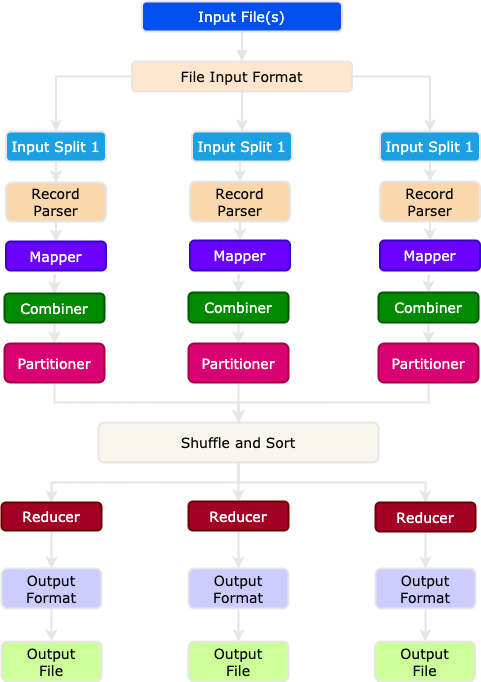
\includegraphics[height=.925\textheight]{./Figures/chapter-02/Map-Reduce.png}
				\caption{Map Reduce Stages } \label{fig:MRSteps}
	\end{figure}			
\end{frame}
%%%%%%%%%%%%%%%%%%%%%%%%%%%%%%%%%%%%%%%%%%%%%%%%%%%%%%
\begin{frame}
	
	\begin{figure}
		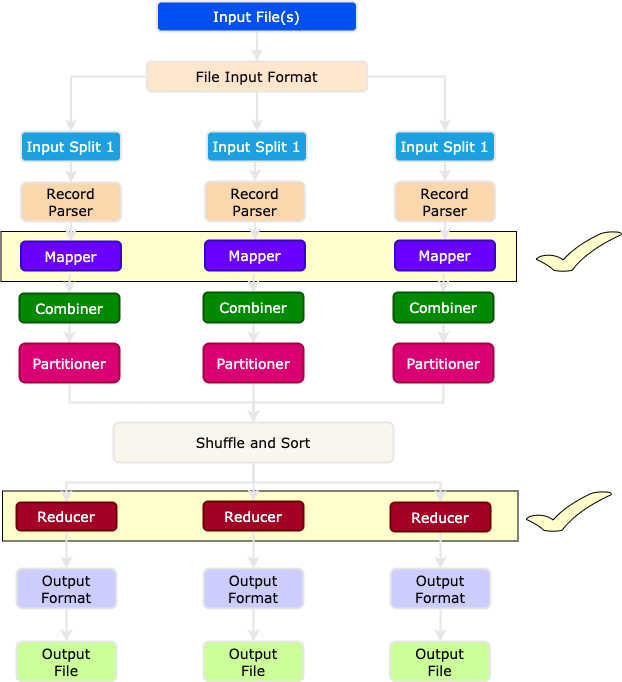
\includegraphics[height=.925\textheight]{./Figures/chapter-02/Map-Reduce_2.png}
		\caption{Map Reduce Stages } \label{fig:MRSteps2}
	\end{figure}			
\end{frame}
%%%%%%%%%%%%%%%%%%%%%%%%%%%%%%%%%%%%%%%%%%%%%%%%%%%%%%
\begin{frame}[c]{ }
	\frametitle{Map Reduce (word count) Deep Dive }
	
	The Map-Reduce consists of three "main" parts
	
	\begin{itemize}  [<+->]
		\item [--] The Driver.
		\item [--] The Mapper.
		\item [--] The Reducer.
		
	\end{itemize}
\end{frame}
%%%%%%%%%%%%%%%%%%%%%%%%%%%%%%%%%%%%%%%%%%%%%%%%%%%%%%
\begin{frame}[c]{ }
	\frametitle{ Hadoop Map Reduce API}
	\centering     
	
	\textcolor{offgreen}{ \large Hadoop Map Reduce API Deep Dive}
\end{frame}
%%%%%%%%%%%%%%%%%%%%%%%%%%%%%%%%%%%%%%%%%%%%%%%%%%%%%%
\begin{frame}[c]{ }
	\frametitle{The Driver }

	\begin{itemize}  [<+->]
		\item [--] The code that runs on the client machine configures the job details by creating an object from the \code{Job}  class, which implements the \code{JobContext} interface.
		\item [--] It submits the job to the cluster.		
		\item [--] It parses job arguments to identify job parameters, for example, input/output directories.. 
		
	\end{itemize}

\end{frame}
%%%%%%%%%%%%%%%%%%%%%%%%%%%%%%%%%%%%%%%%%%%%%%%%%%%%%%
\begin{frame}[c]{ }
	\frametitle{The Driver:  Job Configuration}
	

The \code{Job}  object allows you to set configuration for your \code{Map-Reduce} job:
			\begin{itemize}  [<+->]
				\item [--] You can configure the \code{Mapper} \& the \code{Reducer} classes.
				\item [--] Set the \code{Mapper} input/output key \& value data types.
				\item [--] Set the \code{Reducer} input/output key \& value data types.
	
		
			\end{itemize}		

	
\end{frame}
%%%%%%%%%%%%%%%%%%%%%%%%%%%%%%%%%%%%%%%%%%%%%%%%%%%%%%
\begin{frame}[c]{ }
	\frametitle{The Driver:  Job Configuration}
	
	\begin{itemize}  [<+->]
		\item [--] We can configure file input directory and output.
		\item [--] We configure the output path using \code{FileOutputFormat.setOutputPath()} to specify the reducers' directory to write the output data.
	\end{itemize}		
	
\end{frame}
%%%%%%%%%%%%%%%%%%%%%%%%%%%%%%%%%%%%%%%%%%%%%%%%%%%%%%
\begin{frame}[c]{ }
	\frametitle{The Driver:  Job Configuration}
	
	\begin{itemize}  [<+->]
		\item [--] We configure the input path using \code{FileInputFormat.setInputPaths()}, and by default, it will read all the files in the specified directories and send them to the mappers.
		
		\item [--] We can use \code{Hadoop glob patterns} to read directory patterns, for example, \textit{/warehouse/public/sales*}.
		\item [--] We can call \code{FileInputFormat.addInputPath()} to multiple times by specifying a single file or directory. 
		
	\end{itemize}		
	
	\footnotetext[1]{For more details, please read HTDG. Ch.3 File patterns and PathFilter sections.	} 
\end{frame}
%%%%%%%%%%%%%%%%%%%%%%%%%%%%%%%%%%%%%%%%%%%%%%%%%%%%%%
\begin{frame}[c]{ }
	\frametitle{ Hadoop Map Reduce API}
	\centering     
	
	\textcolor{offgreen}{ \large Please read HTDG. Ch.3 The Java Interface}
\end{frame}
%%%%%%%%%%%%%%%%%%%%%%%%%%%%%%%%%%%%%%%%%%%%%%%%%%%%%%


\begin{frame}[c]{ }
	\frametitle{The Driver:  Job Configuration }
	
		
		\begin{itemize}  [<+->]

			\item [--] You could set driver configurations globally using Hadoop configurations.
			\item [--] Any options not specified in the job configuration will use the Hadoop default values.
			\item [--] We use the \code{Job} object to specify the job name and check its state..
		
			
	\end{itemize}
	
\end{frame}
%%%%%%%%%%%%%%%%%%%%%%%%%%%%%%%%%%%%%%%%%%%%%%%%%%%%%%
\begin{frame}[c]{ }
	\frametitle{The Driver:  Job Configuration }
	

	\begin{itemize}  [<+->]
		
	\item [--] It is optional to set the mapper and reducer classes.
	\item [--] Hadoop uses its default \code{IdentityMapper} and \code{IdentityReducer}.		
		
	\end{itemize}
	
\end{frame}
%%%%%%%%%%%%%%%%%%%%%%%%%%%%%%%%%%%%%%%%%%%%%%%%%%%%%%
\begin{frame}[c]{ }
	\frametitle{The Driver:  Job Configuration }
	
	
	Lunch a Map-Reduce job:
	\begin{itemize}  [<+->]
		
		\item [--] The \code{waitForCompletion()} method in the \code{Job} class launches the job and polls for progress. In addition, it writes the logs and summarizing the Map-Reduce job progress and changes.

	\item [--] When the job completes successfully, the job counters are displayed. Otherwise, the error that caused the job to fail is logged to the console.
		
	\end{itemize}
	
\end{frame}
%%%%%%%%%%%%%%%%%%%%%%%%%%%%%%%%%%%%%%%%%%%%%%%%%%%%%%
\begin{frame}[c]{ }
	\frametitle{InputFormat}
	
	\begin{itemize}  [<+->]
		\item [--] TheThe driver defines the \code{InputFormat}; then the \code{InputFormat} creates a \code{RecordReader"} object that parses the input data into key/value pairs passed to the mapper.
		\item [--] For example: \code{TextInputFormat}:
		\begin{itemize}  [<+->]
			
			\item It is the default.
			\item It creates \code{LineRecordReader} objects.
			\item Key: is the line offest in the file.
			\item Value: is the line which terminated by "\textbackslash n".
		\end{itemize}		
		
		
	\end{itemize}		
	
\end{frame}
%%%%%%%%%%%%%%%%%%%%%%%%%%%%%%%%%%%%%%%%%%%%%%%%%%%%%%
\begin{frame}[c]{ }
	\frametitle{Keys and Values}
	
	\begin{itemize}  [<+->]
		\item [--] Keys and Values in Hadoop are java \code{Objects} not \code{Java primitives types}.
		\item [--] Values are objects which implement \code{Writable}.
		\item [--] Keys are objects which implement \code{WritableComparable}.

		
	\end{itemize}		
	
\end{frame}
%%%%%%%%%%%%%%%%%%%%%%%%%%%%%%%%%%%%%%%%%%%%%%%%%%%%%%
\begin{frame}[c]{ }
	\frametitle{What is Writable?}
	
	\begin{itemize}  [<+->]
		\item [--] \code{Writable} is an interface in Hadoop.
		\item [--] \code{Writables} are used for data type "serialization" in Hadoop to translate/serialize "primitive java data types" to "Hadoop data types", Ex: int to IntWritable and String to Text.
		\item [--] Hadoop uses the \code{Writable} interface for data transfer in the cluster and network.
		
		
	\end{itemize}		
	
\end{frame}
%%%%%%%%%%%%%%%%%%%%%%%%%%%%%%%%%%%%%%%%%%%%%%%%%%%%%%
\begin{frame}[c]{ }
	\frametitle{What is WritableComparable?}
	
	\begin{itemize}  [<+->]
		\item [--] A \code{WritableComparable} is a \code{Writable} which is also \code{Comparable}.
		\item [--] We can compare two \code{WritableComparables} against each other to determine their \textbf{\underline{\textit{order}}}, for example, we could need to compare the order of two Text "Apple vs. Cat or numbers ordering" to understand the ordering mechanism. 
		\item [--] Obviously, the reason we have Keys to be \code{WritableComparable} is that they are passed to the reducer in \underline{\textit{\textbf{sorted order}}}.
		\item [--] Note: All Hadoop implemented types are both \code{Writable} and \code{WritableComparable}.
		
		
	\end{itemize}		
	
\end{frame}
%%%%%%%%%%%%%%%%%%%%%%%%%%%%%%%%%%%%%%%%%%%%%%%%%%%%%%
\begin{frame}[c]{ }
	\frametitle{Map Reduce (word count) Deep Dive }
	
	The Map-Reduce example consists of three main parts
	
	\begin{itemize}  [<+->]
		\item [--] \sout{The Driver}.
		\item [--] The Mapper.

		
	\end{itemize}
\end{frame}
%%%%%%%%%%%%%%%%%%%%%%%%%%%%%%%%%%%%%%%%%%%%%%%%%%%%%%
\begin{frame}[c]{ }
	\frametitle{The Mapper}
		
	\begin{itemize}  [<+->]
		
		\item [--] The mapper class deals with a single input split.
		
		\item [--] All mapper classes must extend the \code{Mapper} base class.

		\item [--] All mapper must specify the key and values for input and output.		
		
		\item [--] All mappers must override the \code{map} method and pass the key, value, and \code{Context}.
		
		\item [--]  The \code{Context} is used to write intermediate data and all information about the job's configurations.
		
	\end{itemize}
	
\end{frame}
%%%%%%%%%%%%%%%%%%%%%%%%%%%%%%%%%%%%%%%%%%%%%%%%%%%%%%
\begin{frame}[c]{ }
	\frametitle{Map Reduce (word count) Deep Dive }
	
	The Map-Reduce example consists of three main parts
	
	\begin{itemize}  [<+->]
		\item [--] \sout{The Driver}.
		\item [--] \sout{The Mapper}.
		\item [--] The Reducer.
		
	\end{itemize}
\end{frame}
%%%%%%%%%%%%%%%%%%%%%%%%%%%%%%%%%%%%%%%%%%%%%%%%%%%%%%
\begin{frame}[c]{ }
	\frametitle{The Reducer}
	
	\begin{itemize}  [<+->]
		
		\item [--] The Reducer receives a Key and an Iterable collection of Writable objects. It also receives a Context object.
		
		\item [--] All reducers classes must extend the  \code{Reducer} base class.
		
		\item [--] All mapper must specify the key and values for intermediate input and final (or intermediate) output.		
		
		\item [--] All reducers must override the "reduce" method and pass the key, \code{Iterable} and "Context".

	\end{itemize}
	
\end{frame}
%%%%%%%%%%%%%%%%%%%%%%%%%%%%%%%%%%%%%%%%%%%%%%%%%%%%%%
\begin{frame}[c]{ }
	\frametitle{ Hadoop Map Reduce API}
	\centering     
	
	\textcolor{offgreen}{ \large Map Reduce Demo}
\end{frame}


%%%%%%%%%%%%%%%%%%%%%%%%%%%%%%%%%%%%%%%%%%%%%%%%%%%%%%
\begin{frame}[c]{ }
	\frametitle{Map Reduce Components }
	
	The Map-Reduce consists of three "main" parts
	
	\begin{itemize}  [<+->]
		\item [--] The Driver.
		\item [--] The Mapper.
		\item [--] The Reducer.
		
	\end{itemize}
\end{frame}

%%%%%%%%%%%%%%%%%%%%%%%%%%%%%%%%%%%%%%%%%%%%%%%%%%%%%%
\begin{frame}
	
	\begin{figure}
		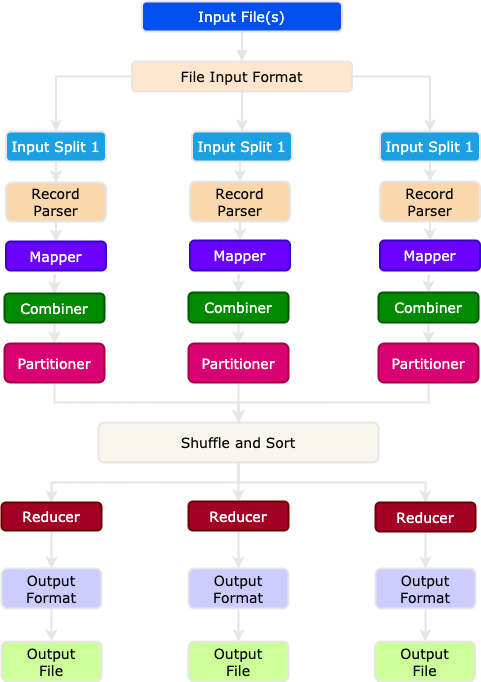
\includegraphics[height=.925\textheight]{./Figures/chapter-02/Map-Reduce.png}
		\caption{Map Reduce Stages } \label{fig:MRSteps}
	\end{figure}			
\end{frame}
%%%%%%%%%%%%%%%%%%%%%%%%%%%%%%%%%%%%%%%%%%%%%%%%%%%%%%
\begin{frame}
	
	\begin{figure}
		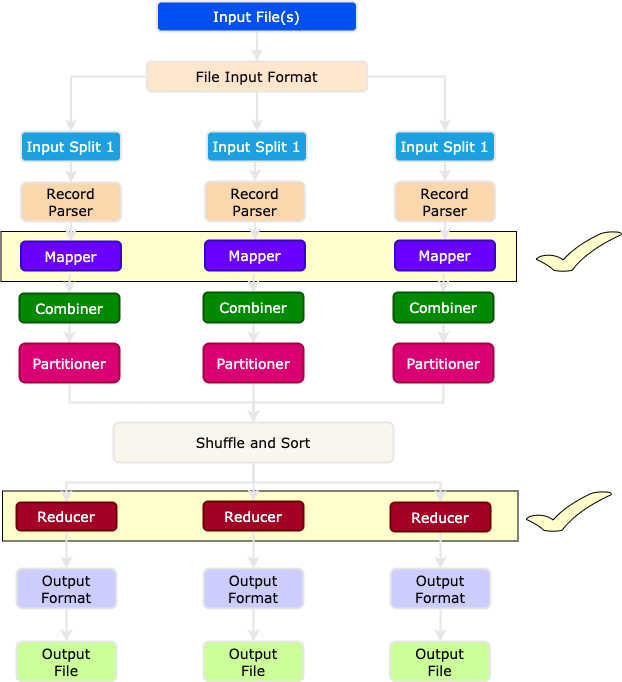
\includegraphics[height=.925\textheight]{./Figures/chapter-02/Map-Reduce_2.png}
		\caption{Map Reduce Stages } \label{fig:MRSteps2}
	\end{figure}			
\end{frame}
%%%%%%%%%%%%%%%%%%%%%%%%%%%%%%%%%%%%%%%%%%%%%%%%%%%%%%
\begin{frame}
	
	\begin{figure}
		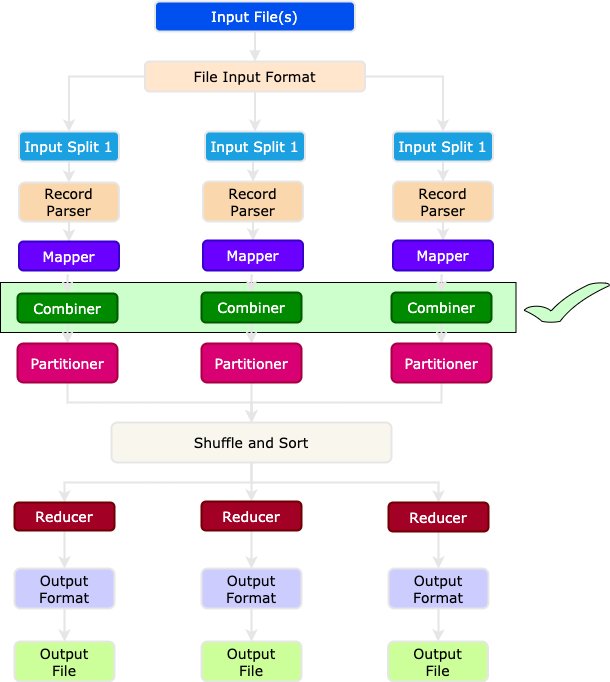
\includegraphics[height=.925\textheight]{./Figures/chapter-02/Map-Reduce-components-combiner.png}
		\caption{Map Reduce Stages } \label{fig:MRSteps2}
	\end{figure}			
\end{frame}

%%%%%%%%%%%%%%%%%%%%%%%%%%%%%%%%%%%%%%%%%%%%%%%%%%%%%%
\begin{frame}[c]{ }
	\frametitle{ The Combiners}
	\centering     
	
	\textcolor{offgreen}{ \large Increase The Map-Reduce Processing Using The Combiners}
\end{frame}
%%%%%%%%%%%%%%%%%%%%%%%%%%%%%%%%%%%%%%%%%%%%%%%%%%%%%%
\begin{frame}
	
	\begin{figure}
		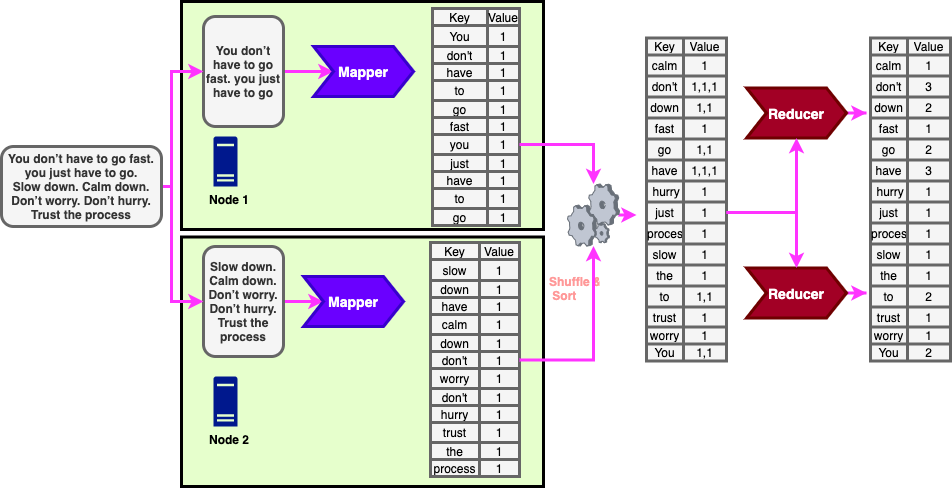
\includegraphics[height=.85\textheight]{./Figures/chapter-02/map-reduce-combiner-ex-1.png}
		\caption{Map Reduce Without Combiner } \label{fig:MRCombiner1}
	\end{figure}			
\end{frame}
%%%%%%%%%%%%%%%%%%%%%%%%%%%%%%%%%%%%%%%%%%%%%%%%%%%%%%
\begin{frame}
	
	\begin{figure}
		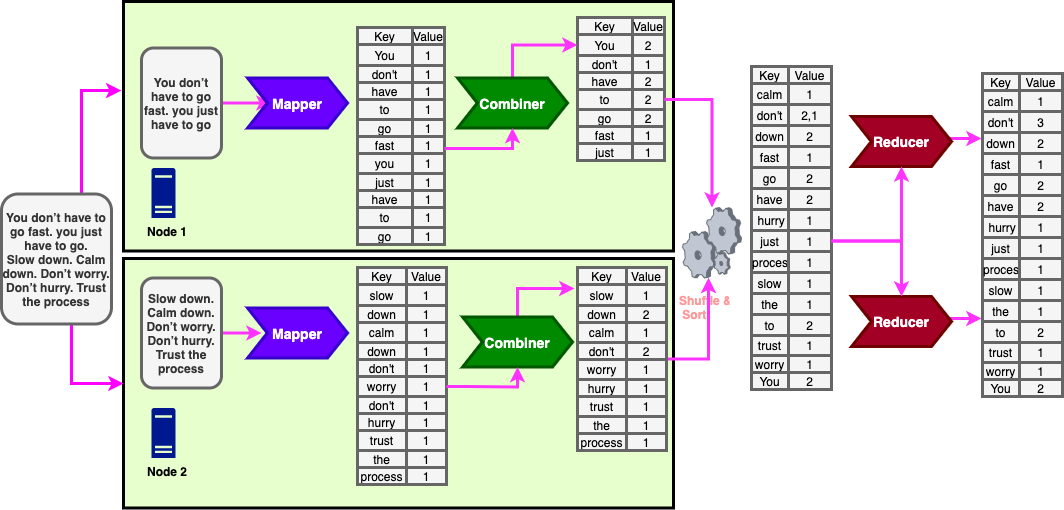
\includegraphics[height=.85\textheight]{./Figures/chapter-02/map-reduce-combiner-ex-2.png}
		\caption{Map Reduce Without Combiner } \label{fig:MRCombiner2}
	\end{figure}			
\end{frame}


%%%%%%%%%%%%%%%%%%%%%%%%%%%%%%%%%%%%%%%%%%%%%%%%%%%%%%%
%\subsection{Further Readings and Assignment}
%
%%%%%%%%%%%%%%%%%%%%%%%%%%%%%%%%%%%%%%%%%%%%%%%%%%%%%%%%%%%%%%%%%%%%%%%%%%%%
%%%% Local Variables:
%%%% mode: latex
%%%% TeX-master: "../main"
%% !TeX root = ../main.tex
%%%% TeX-engine: xetex
%%%% End:
    % use no footline.
% \begin{frame}[plain, noframenumbering]{Outline}
% 	\tableofcontents
% \end{frame}
%%%%%%%%%%%%%%%%%%%%%%%%%%%%%%%%%%%%%%%%%%%%%%%%%%%%%%

% Ch.04-01   | Introduction
\section{Apache Spark}

\begin{frame}
    \frametitle{Course Objectives}

    \begin{itemize}
        \item Understand the fundamentals of Apache Spark.
        \item Build data processing applications using Apache Spark.
        \item Understand Apache Spark APIs (RDD, DataFrames, and Datasets).
        \item Optimize and tune Apache Spark applications.
        \item Build streaming applications using Apache Spark.
        \item Build scalable machine learning applications using Apache Spark MLlib.
        \item Deploy Apache Spark in production environments.
    \end{itemize}

\end{frame}

%%%%%%%%%%%%%%%%%%%%%%%%%%%%%%%%%%%%%%%%%%%%%%%%%%%%%%

\subsection{Course References}
\begin{frame}
    \frametitle{\subsecname}
    \begin{itemize}
        \item \href{https://pages.databricks.com/rs/094-YMS-629/images/LearningSpark2.0.pdf}{Learning Spark, 2nd Edition} By Jules S. Damji, Brooke Wenig, Tathagata Das, Denny Lee.
        \item \href{https://learning.oreilly.com/library/view/spark-the-definitive/9781491912201/}{Spark: The Definitive Guide} By Bill Chambers, Matei Zaharia.
        \item Random blog posts.
    \end{itemize}
\end{frame}
%%%%%%%%%%%%%%%%%%%%%%%%%%%%%%%%%%%%%%%%%%%%%%%%%%%%%%

\subsection{Course Prerequisites}
\begin{frame}
    \frametitle{\subsecname}
    Before beginning this course, participants should have:
    \begin{itemize}
        \item Experience in programming using Python.
        \item Basic programming skills using shell.
        \item An understanding of MapReduce foundations and Hive. \href{https://www.youtube.com/playlist?list=PLxNoJq6k39G8Ak39PDC-oYvp6ZRvIn3Pa}{Garage Education YouTube Playlist}
    \end{itemize}

\end{frame}

%%%%%%%%%%%%%%%%%%%%%%%%%%%%%%%%%%%%%%%%%%%%%%%%%%%%%%

% Ch.04-02   | Python Vs. Scala

\subsection{Python vs Scala}\label{subsec:python-vs-scala}
\begin{frame}
    \frametitle{\subsecname}
    \begin{itemize}
        \item Python is widely used with numerous tools and libraries available.
        \item Python is easier to learn than Scala; however, Scala might be more intuitive for those who prefer functional programming.
        \item Finding Python developers is generally easier for companies than finding Scala developers.
        \item Initially, Scala offered better performance in Apache Spark, but over time this advantage reduced, and now there's no big difference in speed.
        \item PySpark and Scala share the same Spark concepts, allowing for interchangeable use of examples from both languages without affecting learning.
    \end{itemize}
\end{frame}

\begin{frame}
    \begin{center}
        \begin{tcolorbox}[colback=blue!5!white,colframe=blue!75!black,title=Attention!]
            To Be a Spark Expert You Have to Be Able to Read a Little Scala Anyway!\footnote{Referenced from High Performance Spark, 2nd Edition, Ch.01}
        \end{tcolorbox}
    \end{center}

\end{frame}

%
\begin{frame}
    \frametitle{Spark's Codebase and Documentation}
    \begin{itemize}
        \item The quality of Spark's documentation is inconsistent.\footnote{Referenced from High Performance Spark, 2nd Edition, Ch.01}
        \item Spark's codebase is very readable.
        \item Understanding the Spark codebase benefits \textbf{advanced users}.
    \end{itemize}

\end{frame}

\begin{frame}
    \frametitle{Understanding Spark Through Scala}
    \begin{itemize}
        \item Scala helps you understand Spark deeply.\footnote{Referenced from High Performance Spark, 2nd Edition, Ch.01}
        \item Spark is written in Scala.
        \item To work with Spark's source code effectively, it's essential to understand (read) Scala.
    \end{itemize}

\end{frame}

\begin{frame}
    \frametitle{RDD and Scala's Influence}
    \begin{itemize}
        \item Scala's influence is evident in Spark's Resilient Distributed Datasets (RDD).\footnote{Referenced from High Performance Spark, 2nd Edition, Ch.01}
        \item RDD methods are similar to Scala's collection tools.
        \item Functions like map, filter, and reduce are similar in both.
        \item Knowing Scala makes it easier to understand how RDDs work.
    \end{itemize}

\end{frame}

\begin{frame}
    \frametitle{Spark as a Functional Framework}
    \begin{itemize}
        \item Spark uses functional programming principles.
        \item Concepts like immutability and lambda are key.
        \item Understanding functional programming helps in using Spark well.\footnote{Referenced from High Performance Spark, 2nd Edition, Ch.01}
    \end{itemize}

\end{frame}

%%%%%%%%%%%%%%%%%%%%%%%%%%%%%%%%%%%%%%%%%%%%%%%%%%%%%%


%%%%%%%%%%%%%%%%%%%%%%%%%%%%%%%%%%%%%%%%%%%%%%%%%%%%%%
% Ch.04-03   | Introduction

\subsection{Introduction to Apache Spark}\label{subsec:history-of-apache-spark}
\begin{frame}
    \frametitle{\subsecname}
    \begin{itemize}
        \item Apache Spark was initiated at UC Berkeley in 2009, leading to the publication of \href{https://www1.icsi.berkeley.edu/pubs/networking/ICSI_sparkclustercomputing10.pdf}{Spark: Cluster Computing with Working Sets} in 2010 by Matei Zaharia et al.
%    \item It aimed to address the limitations of Hadoop MapReduce, especially for iterative machine learning algorithms requiring multiple data passes. 
        \item Spark was developed to improve processing efficiency over Hadoop MapReduce, which struggled with iterative tasks because it launched separate jobs and reloaded data for each one. This was particularly important for machine learning algorithms that need multiple data passes.
        \item Initially, Spark was designed for batch applications, but it quickly expanded to include streaming, SQL analytics, graph processing, and machine learning.
    \end{itemize}
\end{frame}
\begin{frame}
    \frametitle{\subsecname}
    \begin{itemize}
        \item By 2013, the project had more than 100 contributors, and now it has over 2,000 contributors with more than 39,000 commits. It has been donated to the Apache Software Foundation, guaranteeing its future as a vendor-independent project.
        \item Key milestones in its development are Spark 1.0 in 2014, Spark 2.0 in 2016, and Spark 3.0 in 2020, highlighting its evolution and broad acceptance.
    \end{itemize}
\end{frame}
\begin{frame}
    \frametitle{\subsecname}
    \begin{itemize}
        \item Apache Spark is a \textbf{unified engine} designed for large-scale distributed data processing, either on-premises in data centers or in the cloud.
        \item Spark provides \textbf{in-memory} storage for intermediate computations, making it much faster than Hadoop MapReduce.
        \item Spark offers rich, composable APIs, for example:
        \begin{itemize}
            \item Spark SQL: SQL for interactive queries.
            \item MLlib: for machine learning over big data and complex computations.
            \item Structured Streaming: for stream processing with near real-time data.
            \item GraphX: for graph processing.
        \end{itemize}
        \item \textbf{Optimized Execution Engine}: Spark's Catalyst optimizer and \texttt{Tungsten execution engine} optimize execution plans and generate efficient code for execution.
    \end{itemize}
\end{frame}

%Ch.04-04   | About Databricks

\subsection{About Databricks}\label{subsec:about-databricks}
\begin{frame}
    \frametitle{About Databricks}
    \begin{itemize}
        \item Databricks, founded by the early AMPlab team, joined the community to further develop Spark.
        \item The organization was founded to deliver a comprehensive analytics platform, streamlining Spark's application in big data processing and analytics.
        \item Databricks has bridged the gap between academic research and enterprise applications through its managed cloud service and significant contributions to the Spark project.
    \end{itemize}
\end{frame}
\begin{frame}
    \frametitle{Beyond Apache Spark}
    \begin{minipage}{\textwidth}
        \begin{tikzpicture}
            % Place image at the left side
            \node[anchor=west] (image) at (0,0) {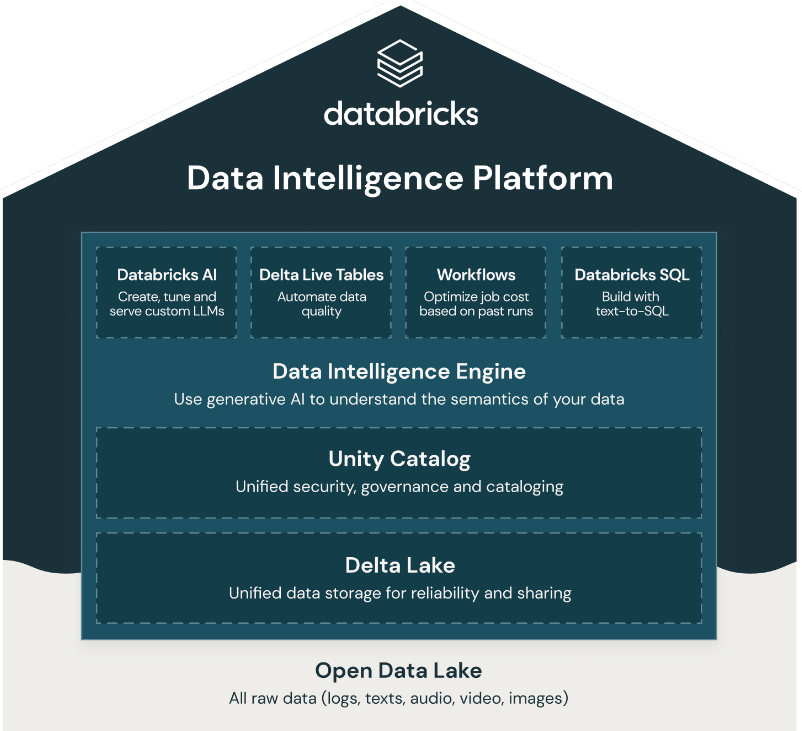
\includegraphics[width=\textwidth,height=.75\textheight,keepaspectratio]{./Figures/chapter-04/databricks_data_intelligence}};
            % Place text and arrow
            \draw[<-, thick] (image) -- ++(4,1) node[right, align=left,font=\small, text=gray] {Photo copied from\\ \url{https://www.datanami.com}};
        \end{tikzpicture}
        \captionof{figure}{Databricks Analytics Platform}
    \end{minipage}
\end{frame}

\begin{frame}
    \centering
    \vfill
    \Large{Do You Need Databricks to Work with Spark?} % Question in normal color
    \vspace{1em} % Add some vertical space before the answer
%\Large{\textcolor{red}{\textbf{NO}}} % Answer "NO" in red and bold for emphasis
    \vfill
\end{frame}

\begin{frame}
    \centering
    \vfill
    \Large{Do You Need Databricks to Work with Spark?} % Question in normal color
    \hspace{1cm} % Add some vertical space before the answer
    \Large{\textcolor{blue}{The answer is NO!}} % Answer "NO" in red and bold for emphasis
    \vfill
\end{frame}
\begin{frame}
    \centering
    \vfill
    \Large{Databricks is one of the cloud options to run Apache Spark workload} % Question in normal color
    \hspace{1cm} % Add some vertical space before the answer
    %\Large{\textcolor{blue}{The answer is NO!}} % Answer "NO" in red and bold for emphasis
    \vfill
\end{frame}
\begin{frame}
    \frametitle{Do You Need Databricks to Work with Spark?}

    \begin{itemize}
        \item Spark workloads can be run both on the Cloud and on-premise.
        \begin{itemize}
            \item \textbf{Cloud:} Choose any preferred cloud provider, like AWS, GCP, Databricks, or Azure.
            \item \textbf{On-Premise:} Deploy on YARN, Mesos, or Kubernetes.
            \item \textbf{Serverless Platforms:} For efficient resource management, consider options like:
            \begin{itemize}
                \item \textbf{AWS:} EMR Serverless or AWS Glue.
                \item \textbf{GCP:} Dataproc.
                \item \textbf{Azure:} Azure Synapse.
                \item \textbf{Databricks:} Databricks analytics platform.
            \end{itemize}
        \end{itemize}
    \end{itemize}
\end{frame}

%%%%%%%%%%%%%%%%%%%%%%%%%%%%%%%%%%%%%%%%%%%%%%%%%%%%%%
% Ch.04-05   | Spark In The Data Platforms

\subsection{Apache Spark in Data Platforms}\label{subsec:apache-spark-in-data-platforms}

\begin{frame}{Technical components in a data lake}
    \begin{minipage}{\textwidth}
        \begin{tikzpicture}
            % Place image at the left side
            \node[anchor=west] (image) at (0,0) {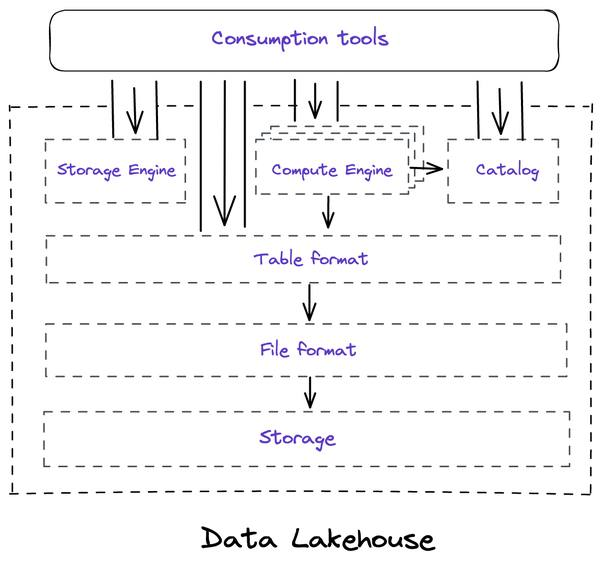
\includegraphics[width=\textwidth,height=.75\textheight,keepaspectratio]{./Figures/chapter-03/datalake_table_format}};
            % Place text and arrow
            \draw[<-, thick] (image) -- ++(4,1) node[right, align=left,font=\small, text=gray] {Apache Iceberg: The Definitive Guide: \\Data Lakehouse Functionality,\\ Performance, and Scalability\\ on the Data Lake\\ PUBLISHED BY:
            O'Reilly Media, Inc.};
        \end{tikzpicture}
        \captionof{figure}{Technical components in a data lake}
    \end{minipage}
\end{frame}

%%%%%%%%%%%%%%%%%%%%%%%%%%%%%%%%%%%%%%%%%%%%%%%%%%%%%%
\begin{frame}{Technical components in a data lake}
    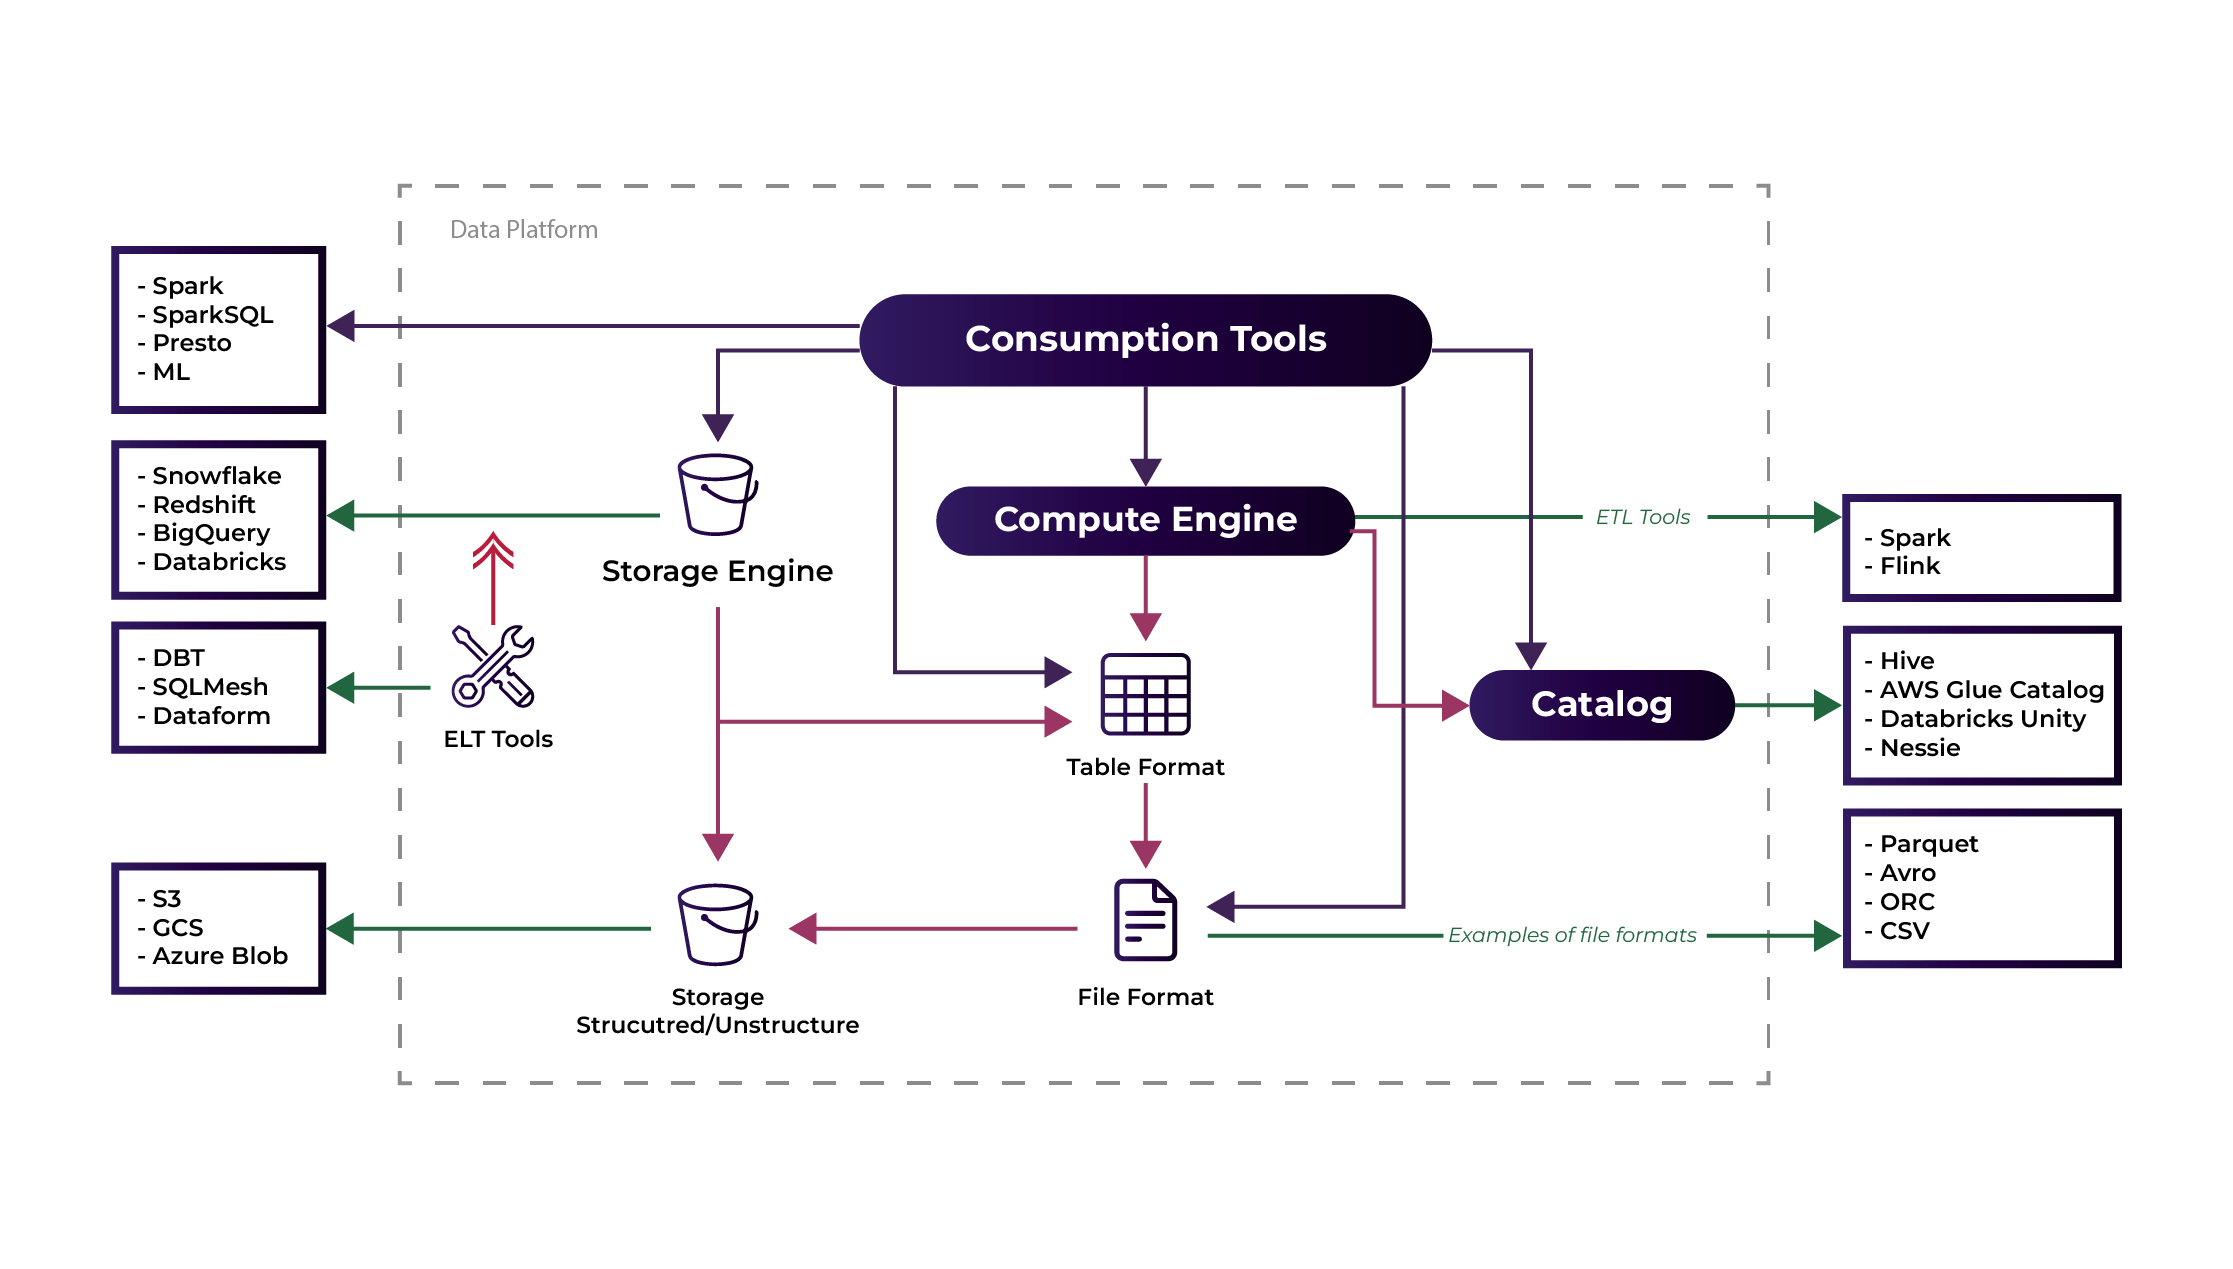
\includegraphics[width=\textwidth,height=.8\textheight,keepaspectratio]{./Figures/chapter-04/DataPlatform};
\end{frame}
%%%%%%%%%%%%%%%%%%%%%%%%%%%%%%%%%%%%%%%%%%%%%%%%%%%%%%
%Ch.04-06   | Running Spark

\subsection{Running Spark}\label{subsec:running-spark}
\begin{frame}
    \frametitle{Running Spark for Beginners}

    \begin{itemize}
        \item \textbf{Databricks Community Edition:} The simplest option for Spark beginners. A free version that's easy to use for learning and small projects.
        \item \textbf{Install Spark Locally:} For hands-on experience with Spark's core features on your own machine.
        \item \textbf{Spark on Docker:} For a flexible, containerized environment that can replicate a production setup.
    \end{itemize}

    \bigskip % Adds a bit more vertical space

    \emph{Note:} For those new to Spark, starting with the Databricks Community Edition is highly recommended due to its user-friendly interface and comprehensive documentation.

\end{frame}
\begin{frame}
    \centering
    \vfill
    \Large{Demo: Databricks Community Edition!}
    \vfill
\end{frame}

\begin{frame}
    \centering
    \vfill
    \Large{Demo: Install Spark Locally on Mac!}
    \vfill
\end{frame}

\begin{frame}
    \centering
    \vfill
    \Large{Demo: Install Spark Locally on Windows!}
    \vfill
\end{frame}

\begin{frame}
    \centering
    \vfill
    \Large{Demo: Install Spark Locally on Linux!}
    \vfill
\end{frame}

\begin{frame}
    \centering
    \vfill
    \Large{Demo: Spark Shell!}
    \vfill
\end{frame}

\begin{frame}
    \centering
    \vfill
    \Large{Demo: Spark SQL!}
    \vfill
\end{frame}
%%%%%%%%%%%%%%%%%%%%%%%%%%%%%%%%%%%%%%%%%%%%%%%%%%%%%%
%Ch.04-11   | From Map Reduce To Spark

\subsection{From MapReduce to Apache Spark}\label{subsec:from-mapreduce-to-apache-spark}

%%%%%%%%%%%%%%%%%%%%%%%%%%%%%%%%%%%%%%%%%%%%%%%%%%%%%%
\begin{frame}
    \frametitle{The basic idea of MapReduce}
    \begin{itemize}
        [<+->]
        \item Assume we need to launch a high-throughput bulk-production sandwich shop.
        \item This sandwich has a lot of raw ingredients, and our target is to produce the sandwich as quickly as possible.
        \item To make the production very quickly we need to distribute the tasks between the  \textcolor{orange}{\textit{workers}}.
    \end{itemize}
    \footnotetext[1]{This example taken from  \href{https://reberhardt.com/cs110/summer-2018/lecture-notes/lecture-14/}{https://reberhardt.com/cs110/summer-2018/lecture-notes/lecture-14/}    }
\end{frame}
%%%%%%%%%%%%%%%%%%%%%%%%%%%%%%%%%%%%%%%%%%%%%%%%%%%%%%
\begin{frame}
    \frametitle{The basic idea of MapReduce}
    We break this into three stages
    \begin{itemize}
        [<+->]
        \item Map.
        \item Shuffle/Group (Mapper Intermediates).
        \item Reduce
    \end{itemize}
    \footnotetext[1]{This example taken from  \href{https://reberhardt.com/cs110/summer-2018/lecture-notes/lecture-14/}{https://reberhardt.com/cs110/summer-2018/lecture-notes/lecture-14/}    }
\end{frame}
%%%%%%%%%%%%%%%%%%%%%%%%%%%%%%%%%%%%%%%%%%%%%%%%%%%%%%
\begin{frame}
    \frametitle{Map}
    We distribute our raw ingredients amongst the workers.
    \begin{figure}
        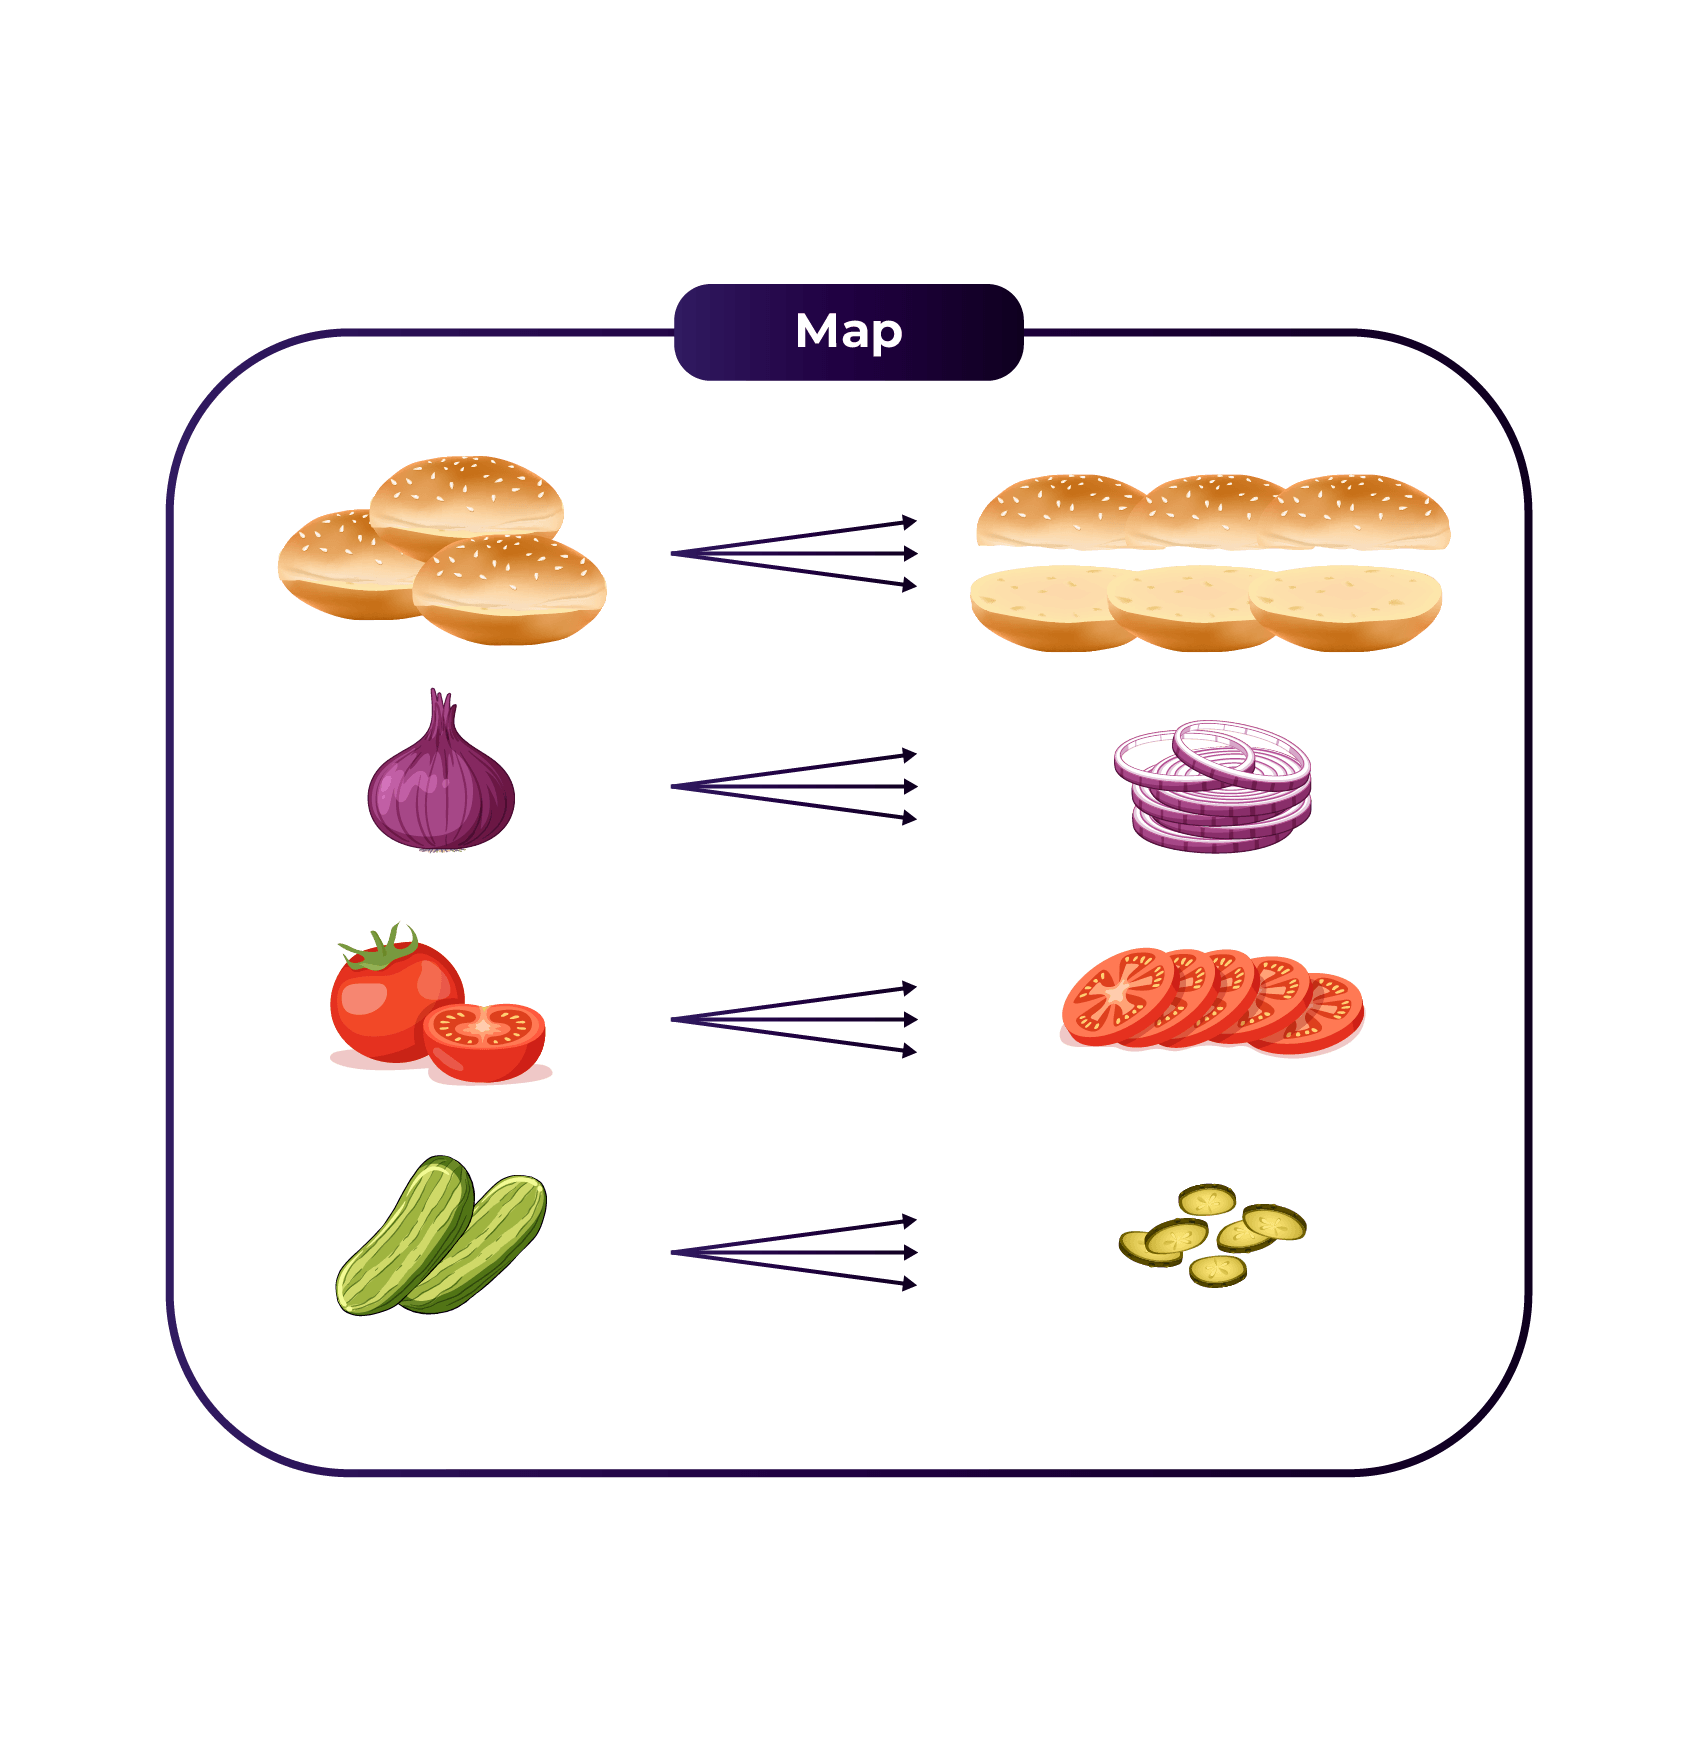
\includegraphics[width=.5\textwidth,height=.8\textheight]{./Figures/chapter-04/map}\label{fig:map}
    \end{figure}
    \footnotetext[1]{{\tiny This example taken from  \href{https://reberhardt.com/cs110/summer-2018/lecture-notes/lecture-14/}{https://reberhardt.com/cs110/summer-2018/lecture-notes/lecture-14/}    } }
\end{frame}
%%%%%%%%%%%%%%%%%%%%%%%%%%%%%%%%%%%%%%%%%%%%%%%%%%%%%%
\begin{frame}
    \frametitle{Shuffle/Group}
    We will organise and group the processed ingredients into piles, so that making a sandwich becomes easy.
    \begin{figure}
        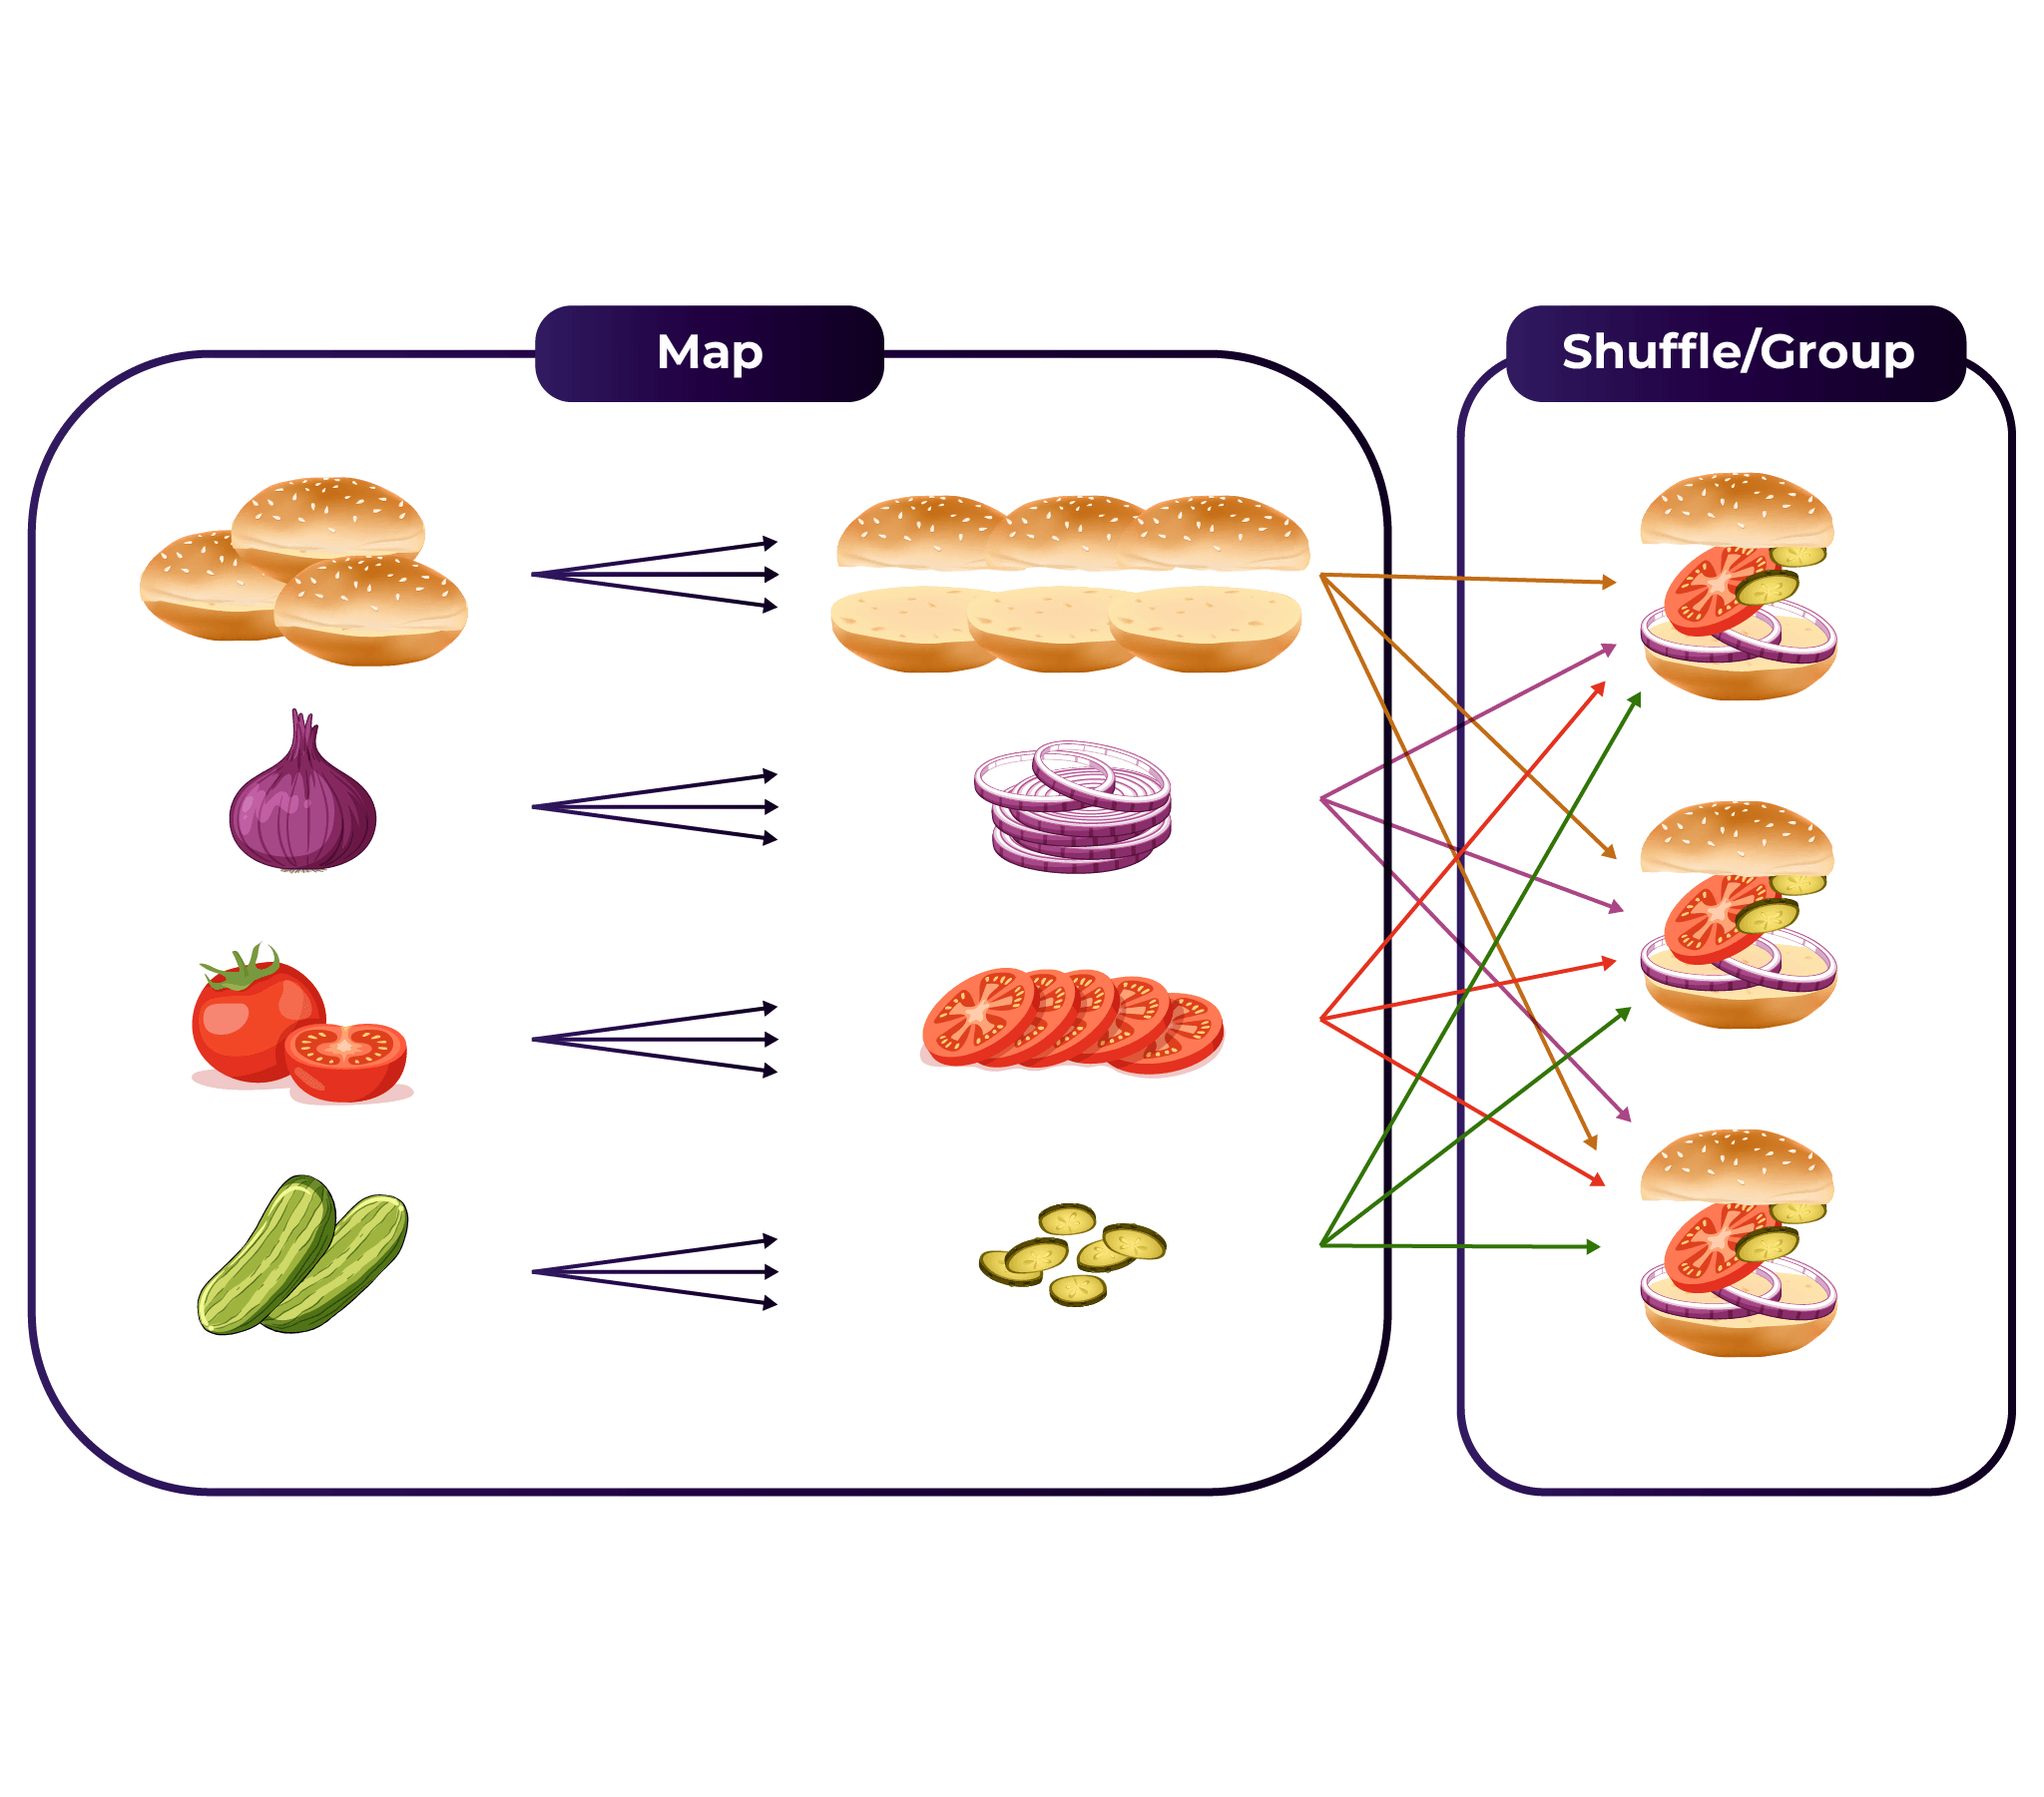
\includegraphics[width=.7\textwidth,height=.8\textheight]{./Figures/chapter-04/map_shuffle}\label{fig:map_shuffle}
    \end{figure}
    \footnotetext[1]{{\tiny This example taken from  \href{https://reberhardt.com/cs110/summer-2018/lecture-notes/lecture-14/}{https://reberhardt.com/cs110/summer-2018/lecture-notes/lecture-14/}    }}
\end{frame}
%%%%%%%%%%%%%%%%%%%%%%%%%%%%%%%%%%%%%%%%%%%%%%%%%%%%%%
\begin{frame}
    \frametitle{Reduce}
    we’ll combine the ingredients into a sandwich
    \begin{figure}
        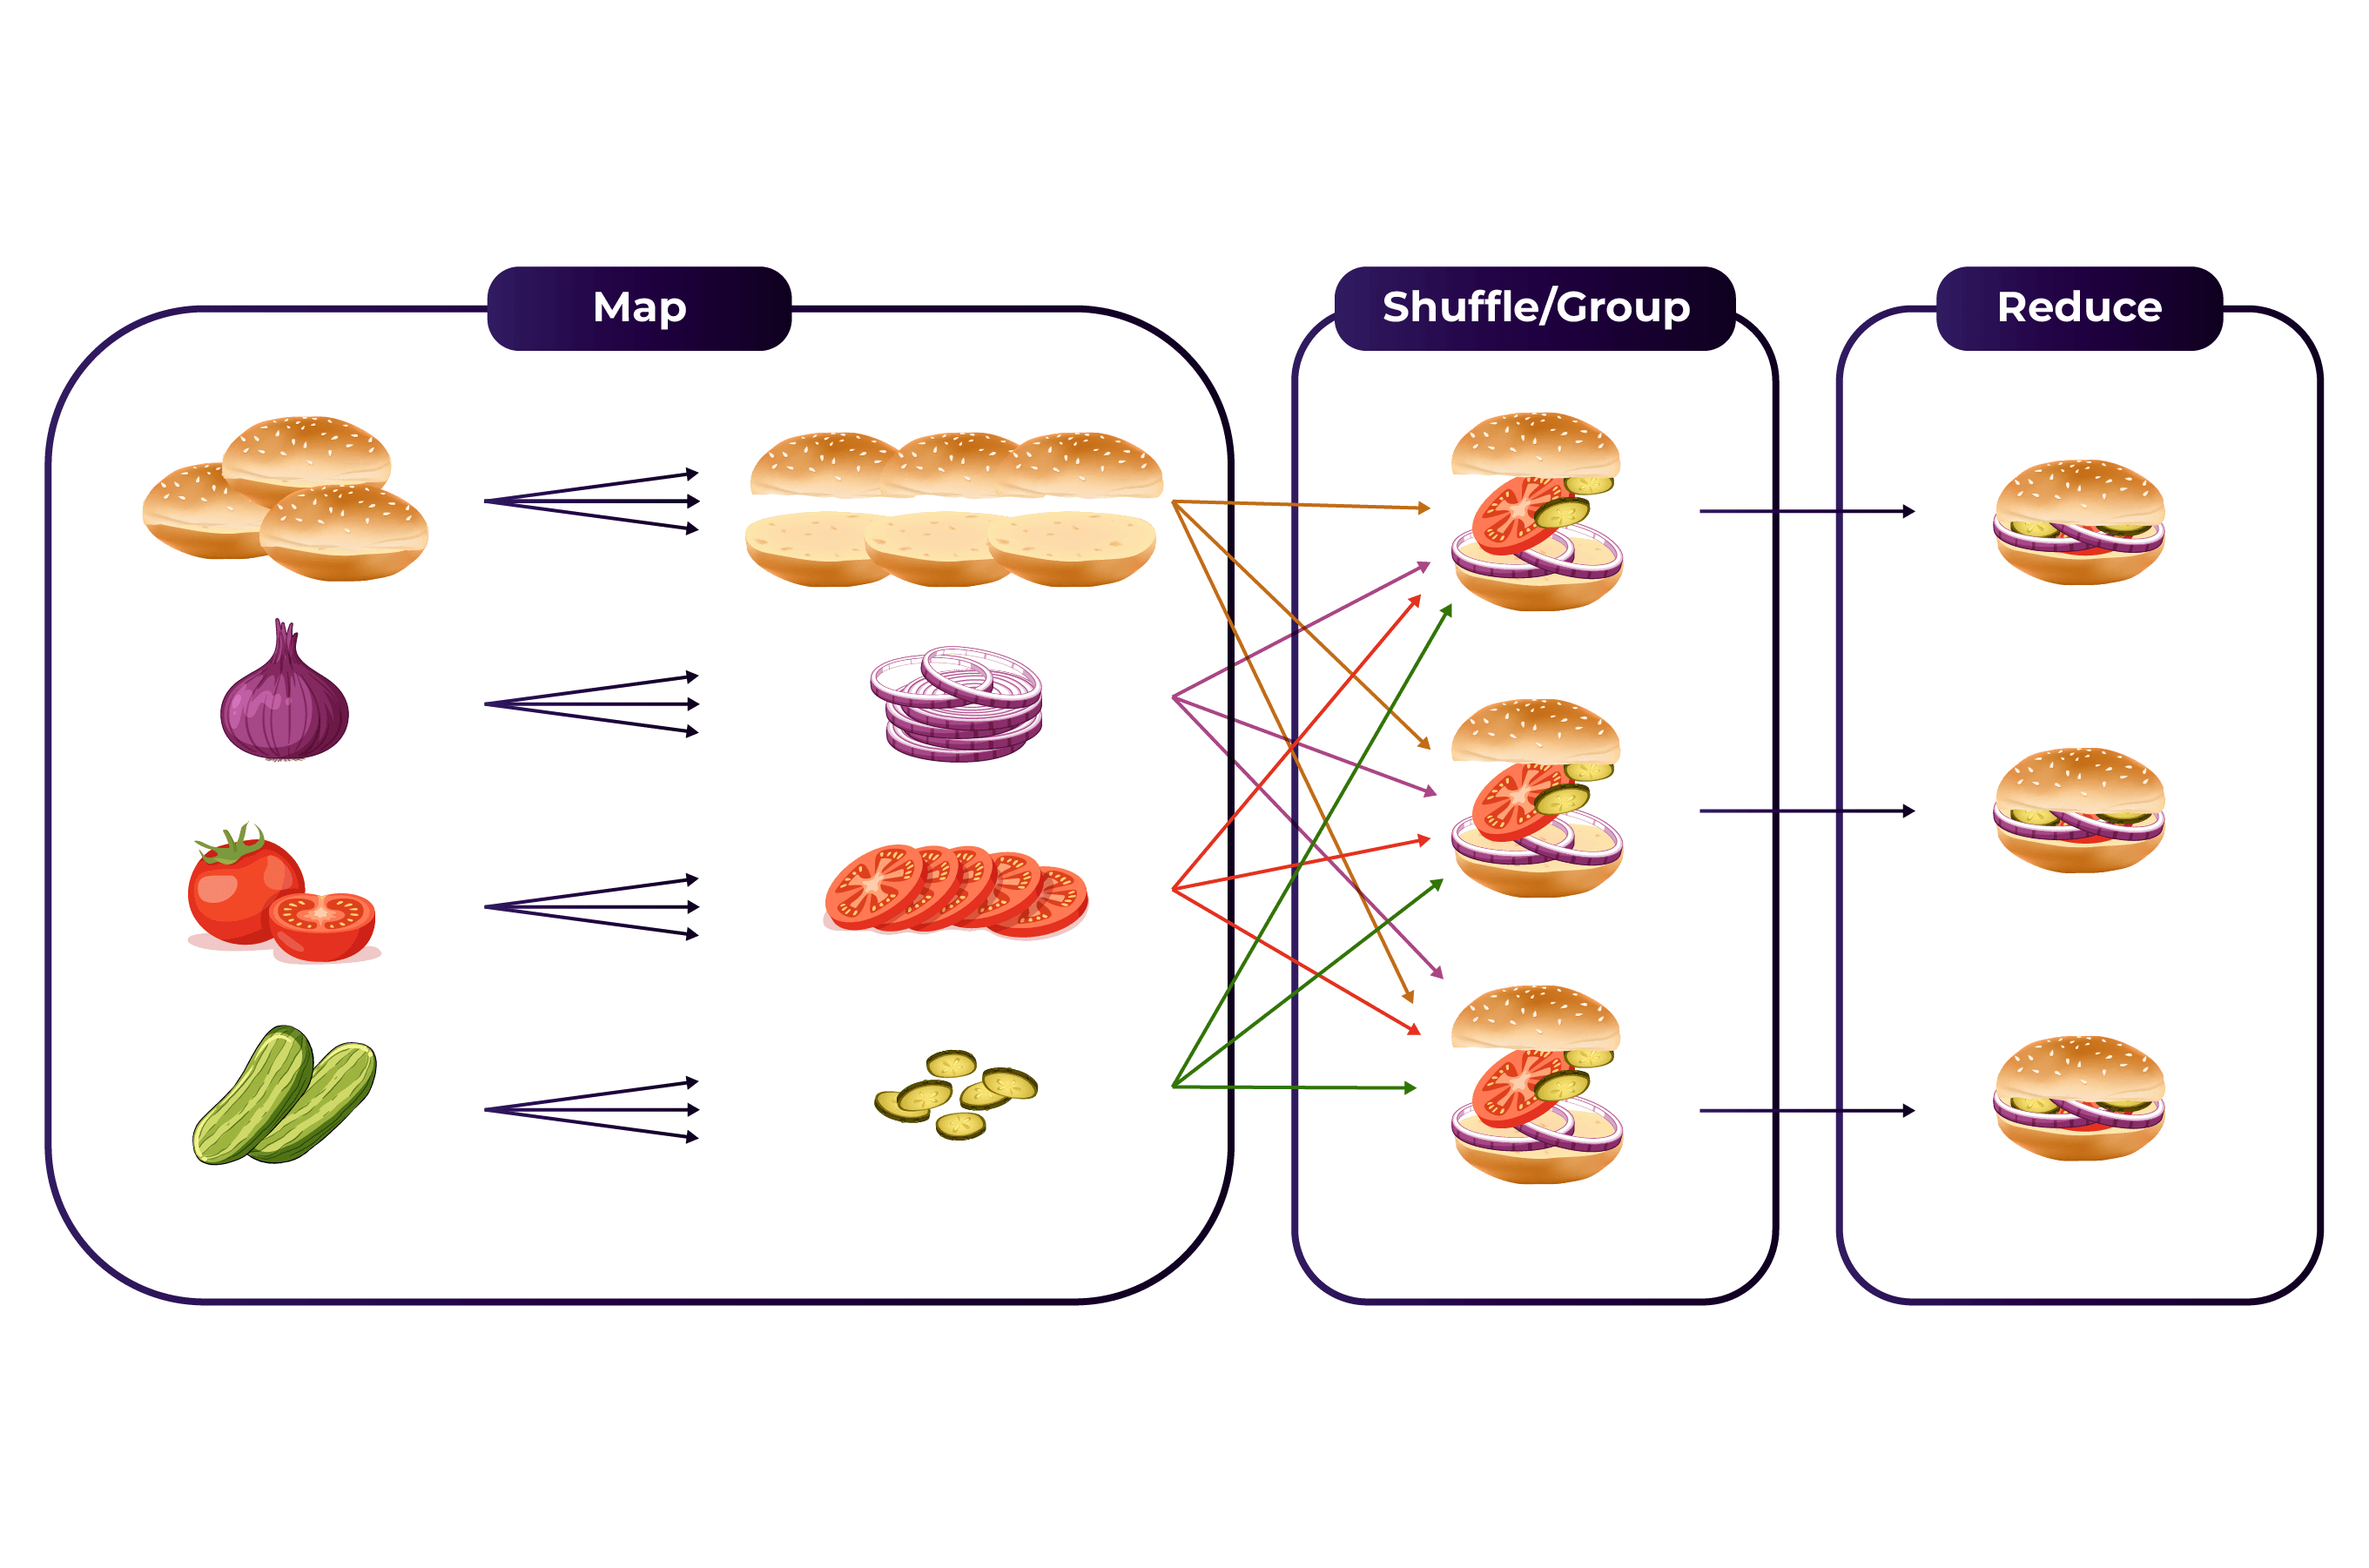
\includegraphics[width=.96\textwidth,height=.6\textheight]{./Figures/chapter-04/map_reduce}\label{fig:map_reduce}
    \end{figure}
    \footnotetext[1]{ {\tiny This example taken from  \href{https://reberhardt.com/cs110/summer-2018/lecture-notes/lecture-14/}{https://reberhardt.com/cs110/summer-2018/lecture-notes/lecture-14/}    }}
\end{frame}
%%%%%%%%%%%%%%%%%%%%%%%%%%%%%%%%%%%%%%%%%%%%%%%%%%%%%%
\begin{frame}
    \frametitle{Map Reduce Bottelneck}
    \begin{figure}
        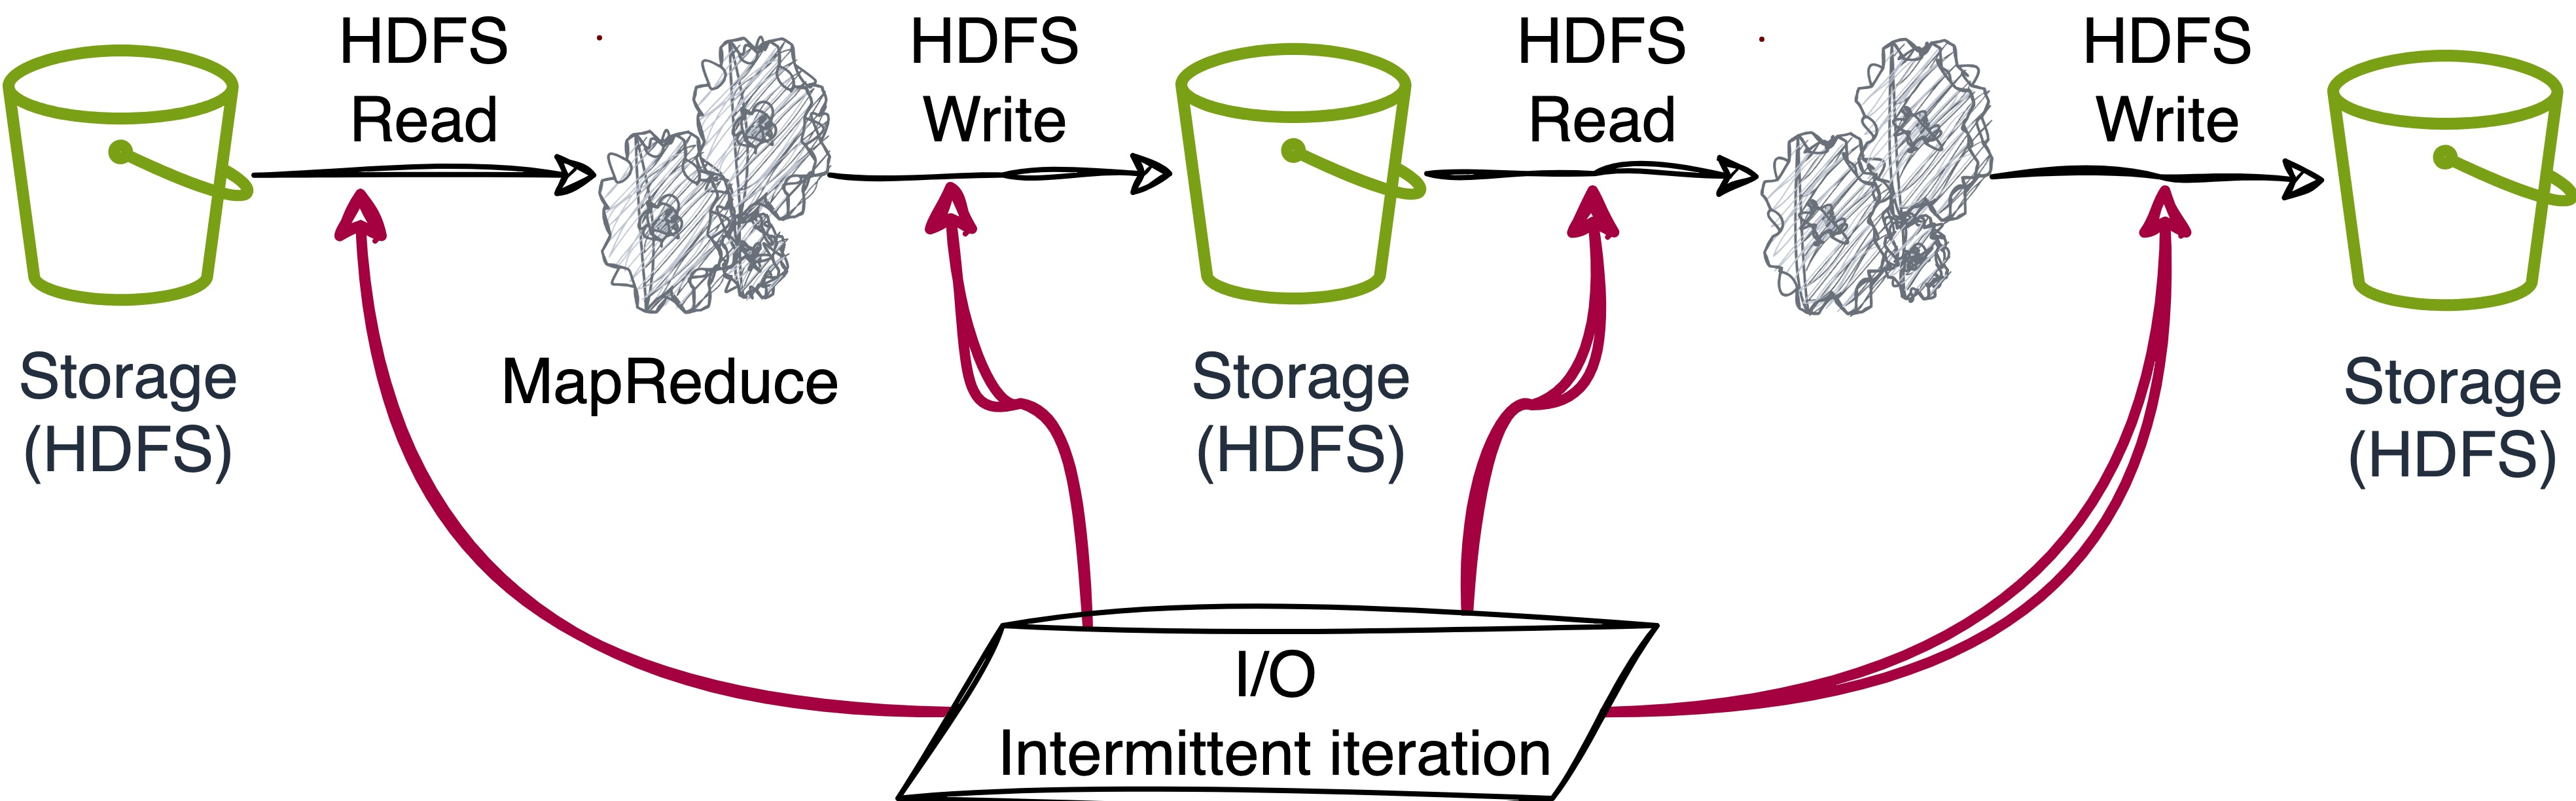
\includegraphics[width=.96\textwidth,height=.6\textheight]{./Figures/chapter-04/MR}\label{fig:figure4}
    \end{figure}
\end{frame}
%%%%%%%%%%%%%%%%%%%%%%%%%%%%%%%%%%%%%%%%%%%%%%%%%%%%%%
\begin{frame}
    \frametitle{Spark Motivation}
    \begin{itemize}

        \item In-Memory Processing.

        \item Resilient Distributed Datasets (RDDs).%**: Spark uses RDDs to perform parallel operations on data stored across cluster nodes, minimizing disk I/O by keeping data in RAM.

        \item Optimized Execution (DAG execution engine).%: The DAG execution engine organizes computations efficiently, reducing unnecessary operations and combining tasks to lower data movement.

        \item Caching.%: Spark allows for the caching of intermediate data in memory, benefiting iterative algorithms that reuse data, thereby avoiding repetitive disk access.

        \item Advanced Optimization (Catalyst optimizer and Tungsten).%: With components like the Catalyst optimizer and Tungsten for memory and CPU efficiency, Spark streamlines execution, making it ideal for fast, iterative processing over big data.

    \end{itemize}
\end{frame}
%%%%%%%%%%%%%%%%%%%%%%%%%%%%%%%%%%%%%%%%%%%%%%%%%%%%%%
% Ch.04-12   | Spark Characteristics

\subsection{Spark Characteristics}\label{subsec:characteristics-apache-spark}

\begin{frame}
    \frametitle{Spark Characteristics}
    \begin{itemize}
        \item Speed.
        \item Ease of use.
        \item Modularity.
        \item Extensibility.
    \end{itemize}
\end{frame}


\begin{frame}
    \frametitle{Spark Characteristics: Speed}
    \begin{itemize}
        \item Spark's speed is achieved through various strategies.
        \begin{itemize}
            \item \textbf{Hardware Utilization:} Spark leverages commodity hardware with extensive memory and multiple cores, utilizing efficient multithreading and parallel processing for improved performance.
            \item \textbf{Directed Acyclic Graph (DAG):} Spark constructs computations as a DAG. Its scheduler and optimizer create an efficient graph, allowing parallel task execution across cluster workers. \textit{\color{blue}This topic will be discussed later.}
            %TODO: about Spark DAG scheduler
        \end{itemize}
    \end{itemize}

\end{frame}

\begin{frame}
    \frametitle{Spark Characteristics: Speed}
    \begin{itemize}
        \item Spark's speed is achieved through various strategies.
        \begin{itemize}
            \item \textbf{Tungsten Execution Engine:} Tungsten enhances Spark's speed by optimizing memory management,
            shifting from JVM-managed objects to direct binary processing, and employing cache-optimized algorithms and advanced code generation. These improvements reduce CPU and memory bottlenecks, significantly boosting performance. \textit{\color{blue}This topic will be discussed later.}
        \end{itemize}
    \end{itemize}

\end{frame}

\begin{frame}
    \frametitle{Spark Characteristics: Ease of use}
    \begin{itemize}
        \item Spark simplifies big data processing with an abstraction called a Resilient Distributed Dataset (RDD).
        \item RDDs serve as the foundation for higher-level data structures like DataFrames and Datasets in Spark. \textit{\color{blue}This topic will be discussed later.}
        \item Compared with MapReduce and other complex distributed processing frameworks, Spark provides a simple programming model with a range of transformations and actions.
    \end{itemize}
\end{frame}


\begin{frame}
    \frametitle{Spark Characteristics: Modularity}
    \begin{itemize}
        \item Spark operations are flexible, supporting various workloads and languages: Scala, Java, Python, SQL, and R.
        \item It provides unified libraries with comprehensive APIs (SparkSQL, Structured Streaming, MLlib, and GraphX).
        \item These modules allow Spark to handle different workloads under a single engine.
        \item With Spark, you can develop a single application for diverse tasks without the need for separate engines or learning different APIs, achieving a unified processing framework.
    \end{itemize}
\end{frame}

\begin{frame}
    \frametitle{Spark Characteristics: Extensibility}
    \begin{itemize}
        \item Spark focuses on its fast, parallel computation engine rather than on storage (Unlike Apache Hadoop, which included both storage and compute).
    \end{itemize}
\end{frame}


\begin{frame}
    \frametitle{Spark Characteristics: Extensibility}
    \begin{itemize}
        \item Spark can process data from various sources like Hadoop, Cassandra, HBase, MongoDB, Hive, RDBMSs, and others in memory for faster processing.
        \item Spark's \texttt{DataFrameReader}s and \texttt{DataFrameWriter}s allow Spark to interact with even more data sources, such as Kafka, Kinesis, Azure Storage, and Amazon S3.
        \item The Spark community maintains a list of third-party packages, enhancing its ecosystem with connectors for external data sources, performance monitors, and more.
    \end{itemize}
\end{frame}


%%%%%%%%%%%%%%%%%%%%%%%%%%%%%%%%%%%%%%%%%%%%%%%%%%%%%%


\section{Apache Spark Distributed Execution}\label{sec:apache-spark-distributed-execution}
\begin{frame}
    \frametitle{Spark Distributed Execution}
    \begin{itemize}
        \item Spark Application.
        \item Spark driver.
        \item Spark session.
        \item Cluster manager.
        \item Spark executors.
        \item Deployment mode.
        \item Data partition.
    \end{itemize}
\end{frame}

% Ch.04-13   | Spark Applications

\subsection{Spark Application}\label{subsec:spark-application}
\begin{frame}
    \frametitle{Spark Distributed Execution: Spark Application}

    \begin{itemize}
        \item A Spark application is a program designed for distributed data processing using Spark.
        \item It includes a driver program to run the main function and execute parallel operations on a cluster.
        \item The application divides processing tasks into smaller units called tasks, distributed across cluster nodes.
        \item Spark applications support various languages like Scala, Java, Python, and R.
    \end{itemize}

\end{frame}

\begin{frame}
    \frametitle{Spark Application}

    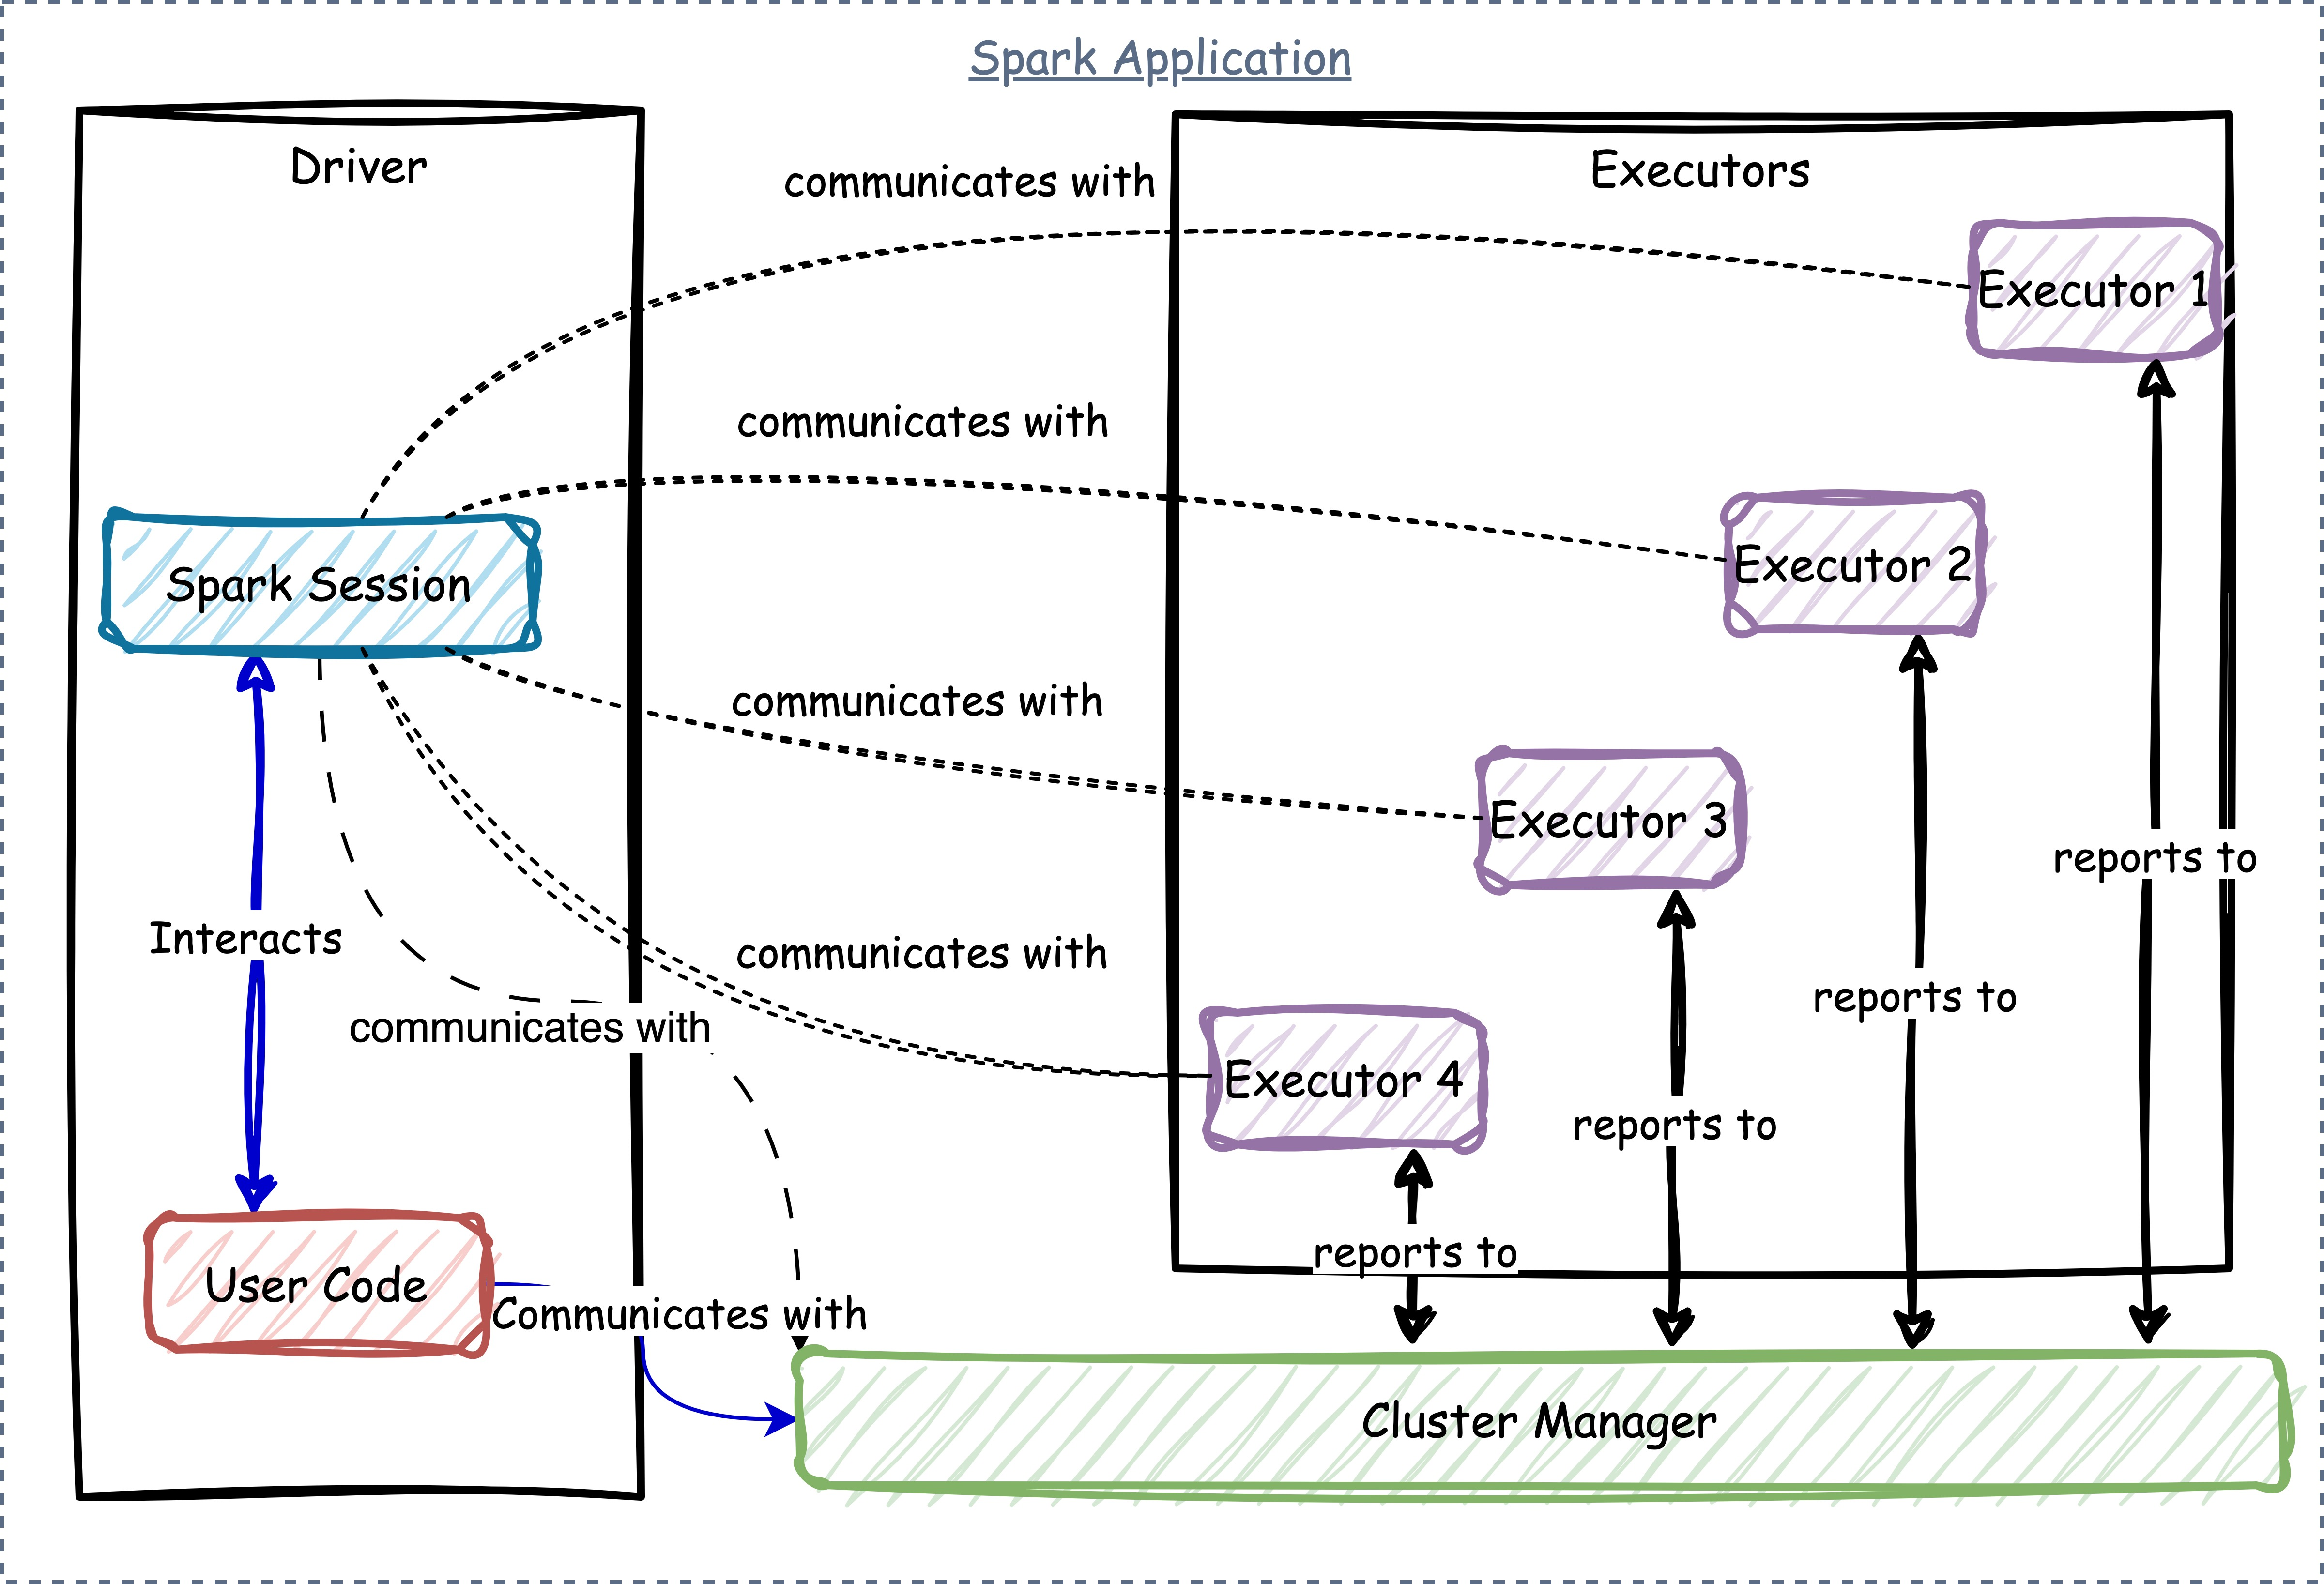
\includegraphics[width=\textwidth,height=.75\textheight,keepaspectratio]{./Figures/chapter-04/SparkCourse.drawio}\footnote{Spark the definitive guide, Ch.02}

\end{frame}

% Ch.04-14   | Spark Driver

\subsection{Spark Driver}\label{subsec:spark-driver}

\begin{frame}
    \frametitle{Spark Driver}
    The driver is the process \texttt{\color{blue}in the driver seat.}\footnote{Spark: The Definitive Guide, Chapter 15.} of your Spark Application.

\end{frame}

\begin{frame}
    \frametitle{Spark Driver: Key functions}


    \begin{itemize}
        \item It transforms all the Spark operations into DAG computations, schedules them, and distributes their execution as tasks across the Spark executors.
        \item Controlling the execution of a Spark Application.

    \end{itemize}

\end{frame}


\begin{frame}
    \frametitle{Spark Driver: Key functions}

    \begin{itemize}
        \item Acting as a process on a physical machine, responsible for the overall state of the application on the cluster.
        \item It instantiates the \texttt{\color{blue} SparkSession}
        \item It requests resources  (CPU, memory, etc.) from the cluster manager for Spark’s executors (JVMs).
        \item Once the resources are allocated, it communicates directly with the executors.
    \end{itemize}

\end{frame}


\begin{frame}
    \frametitle{Spark Driver: Recap}
%graph TD;
%    A[Spark Driver] -->|Schedules Tasks| B(DAG Scheduler);
%    A -->|Request Resources| C(Cluster Manager);
%    A -->|Communicates| D(Executors);
%    A -->|Initiates| E(SparkSession);
%    B -->|Distributes Tasks| D;
%    C -->|Grants Resources| D;
%    D -->|Executes Tasks| F(Task);
%    E -->|User Interface| G(Application Code);
%
    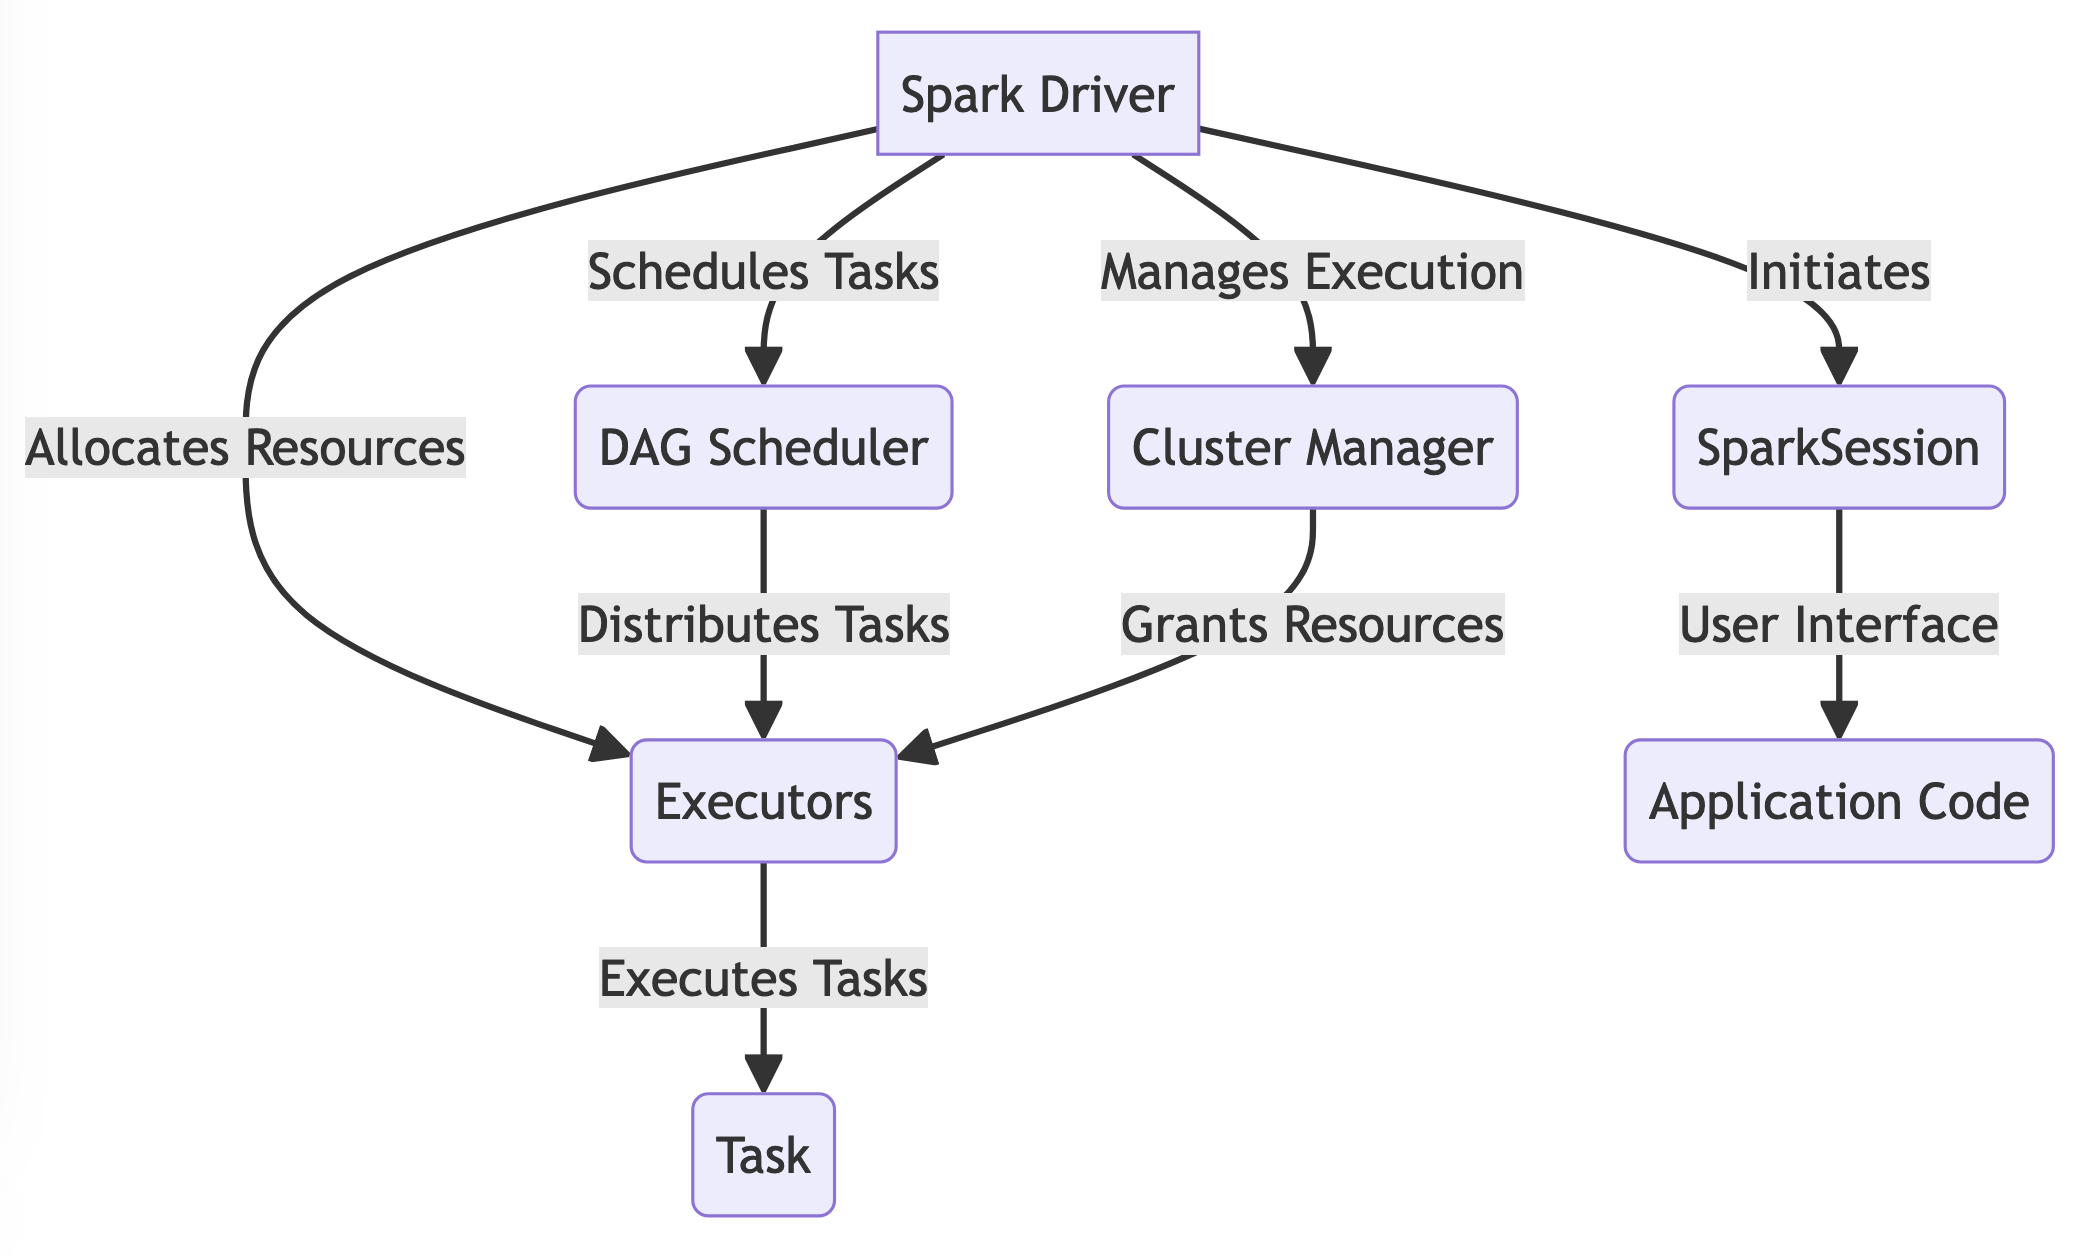
\includegraphics[width=\textwidth,height=.85\textheight,keepaspectratio]{./Figures/chapter-04/Mairmaid_SparkDriver}

\end{frame}

% Ch.04-15   | Spark Session

\subsection{Spark Distributed Execution: SparkSession}\label{subsec:spark-session}
\begin{frame}
    \frametitle{What is a Session?}

    \begin{itemize}
        \item A session refers to an interaction between two or more entities.
        \item In computing, it's especially common in networked computers on the internet.
    \end{itemize}

\end{frame}

\begin{frame}
    \frametitle{Types of Sessions in Computing}

    \begin{itemize}
        \item TCP session: A basic form of interaction in network communication.
        \item Login session: The period when a user is logged into a system.
        \item HTTP session: A series of interactions between a web server and a client.
        \item User session: The time a user interacts with a software application.
    \end{itemize}

\end{frame}

\begin{frame}
    \frametitle{Introducing SparkSession}

    \begin{itemize}
        \item Similar to the sessions mentioned, Spark has its own SparkSession.
        \item SparkSession provides a unified entry point to Spark's functionalities.
    \end{itemize}

\end{frame}

\begin{frame}
    \frametitle{Functionality of SparkSession}

    \begin{itemize}
        \item \textbf{SparkSession:} An object that provides a point of entry to interact with underlying Spark functionality.
        \item It allows programming Spark with its APIs.
        \item In an interactive Spark shell, the Spark driver instantiates a SparkSession for you.
        \item In a Spark application, you create a SparkSession object yourself.
        \item You can program Spark using DataFrame and Dataset APIs through SparkSession.
        \item In Scala and Python, the variable is available as \texttt{spark} when you start the console.

    \end{itemize}
\end{frame}

\begin{frame}
    \frametitle{SparkSession}
    \begin{itemize}
        \item The SparkSession instance is the way Spark executes user-defined manipulations across the cluster.
        \item There is a one-to-one correspondence between a SparkSession and a Spark Application.
        \item It connects the Spark driver program with the cluster manager.
        \item SparkSession determines the resource manager (YARN, Mesos, or Standalone) for communication.
        \item It allows configuration of Spark parameters.
    \end{itemize}
\end{frame}


\begin{frame}[fragile]
    \frametitle{Interacting with Spark in Earlier Versions}

    \begin{itemize}
        \item In earlier versions of Spark, setting up a Spark application required creating a SparkConf and SparkContext.
    \end{itemize}

    \begin{lstlisting}[language=Python,label={lst:pyspark-spark-context},caption={Create SparkContext in old Spark versions}]
from pyspark import SparkConf, SparkContext
from pyspark.sql import SQLContext

sparkConf = SparkConf().setAppName("SparkSessionExample").setMaster("local")
sc = SparkContext(conf=sparkConf)
sqlContext = SQLContext(sc)
    \end{lstlisting}

\end{frame}


\begin{frame}[fragile]
    \frametitle{Interacting with Spark in Earlier Versions}

    \begin{lstlisting}[language=Scala,label={lst:scala-spark-context},caption={Scala: Create SparkContext in old Spark versions}]
//set up the spark configuration and create contexts
val sparkConf = new SparkConf().setAppName("SparkSessionZipsExample").setMaster("local")
val sc = new SparkContext(sparkConf)
sc.set("spark.some.config.option", "some-value")
val sqlContext = new org.apache.spark.sql.SQLContext(sc)
    \end{lstlisting}

\end{frame}


\begin{frame}[fragile]
    \frametitle{Simplification in Spark 2.0 with SparkSession}

    \begin{itemize}
        \item Spark 2.0 introduced SparkSession, simplifying the way you interact with Spark.
        \item SparkSession encapsulates SparkConf, SparkContext, and SQLContext.
    \end{itemize}

    \begin{lstlisting}[language=Python,label={lst:spark-session-python-example},caption={Pyspark: Create SparkSession}]
from pyspark.sql import SparkSession

spark = SparkSession.builder \
    .appName("SparkSessionExample") \
    .config("spark.some.config.option", "value") \
    .getOrCreate()
    \end{lstlisting}

\end{frame}
\begin{frame}[fragile]
    \frametitle{Simplification in Spark 2.0 with SparkSession}
    \begin{lstlisting}[language=Scala,label={lst:spark-session-scala-example},caption={Spark: Create SparkSession}]
// Create a SparkSession. No need to create SparkContext.
val warehouseLocation = "file:${system:user.dir}/spark-warehouse"
val spark = SparkSession
   .builder()
   .appName("SparkSessionZipsExample")
   .config("spark.sql.warehouse.dir", warehouseLocation)
   .enableHiveSupport()
   .getOrCreate()
    \end{lstlisting}
\end{frame}

\begin{frame}
    \frametitle{Using SparkSession}

    \begin{itemize}

        \item Spark 2.0 introduces SparkSession.
        \item With SparkSession, you can access all Spark functionalities.
        \item A unified entry point to Spark's functionality, reduces the need for multiple context initializations.
        \item Encapsulates the functionalities of SQLContext, HiveContext, and more.
    \end{itemize}

\end{frame}

\begin{frame}
    \frametitle{Reference}

    \begin{itemize}
        \item The examples shown are based on a blog post from Databricks.
        \item URL: \url{https://www.databricks.com/blog/2016/08/15/how-to-use-sparksession-in-apache-spark-2-0.html}
    \end{itemize}

\end{frame}

%Ch.04-16   | Spark Cluster Manager

\subsection{Cluster manager}\label{subsec:cluster-manager}

\begin{frame}
    \frametitle{Introduction to Spark Cluster Managers}
    \begin{itemize}
        \item The cluster manager allocates resources for Spark applications.
        \item Supports several managers: Standalone, Hadoop YARN, Apache Mesos, and Kubernetes.
    \end{itemize}
\end{frame}

\begin{frame}
    \frametitle{Role of the Cluster Manager}
    \begin{itemize}
        \item The Spark Driver and Executors do not exist in a void, and this is where the cluster manager
        comes in.
        \item The cluster manager is important for managing a cluster of machines intended to run Spark Applications.
        \item Maintains a \texttt{driver (or master)} and \texttt{worker} nodes, tied to \textbf{physical machines}.
    \end{itemize}
\end{frame}


\begin{frame}
    \frametitle{Cluster Manager Components}
    \begin{figure}
        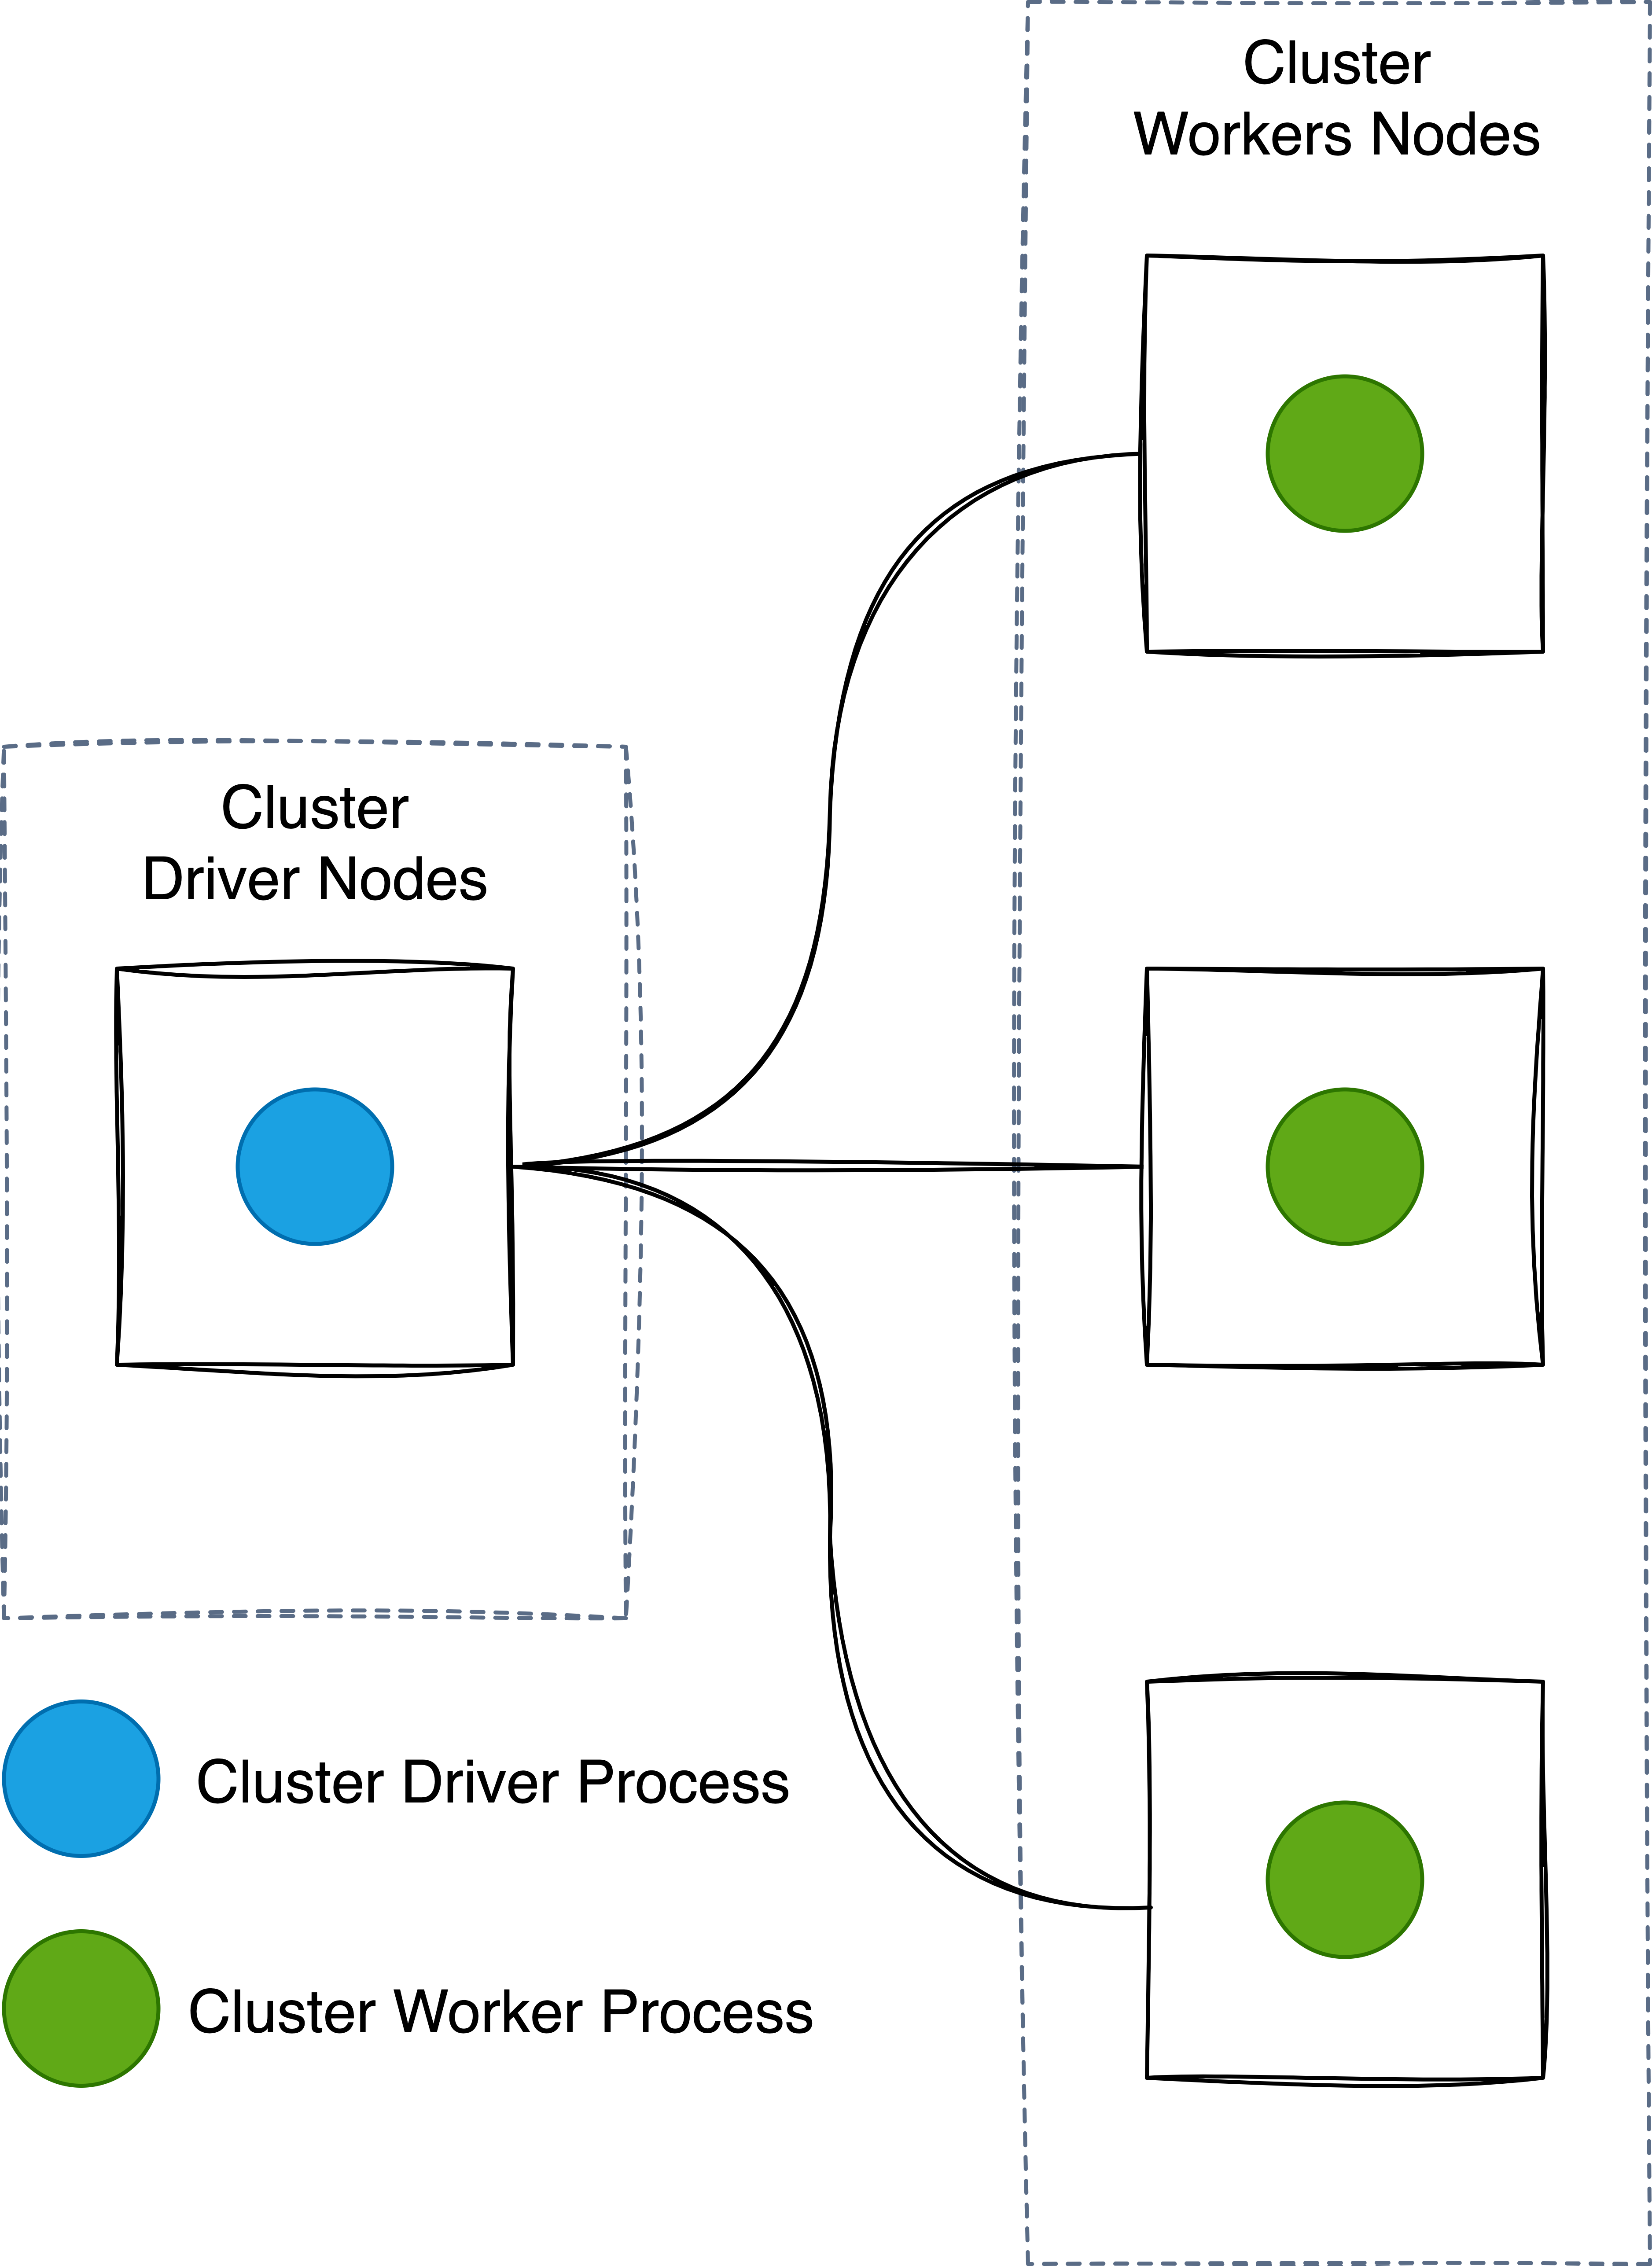
\includegraphics[width=\textwidth,height=.7\textheight,keepaspectratio]{./Figures/chapter-04/cluster_manager_processes}
        \caption{A cluster driver and worker (no Spark Application yet).}\label{fig:cluster_manager_processes}
    \end{figure}
\end{frame}

\begin{frame}
    \frametitle{Execution of Spark Applications}
    \begin{itemize}
        \item The user requests resources from the cluster manager to initiate Spark applications.
        \item The user configures the application to specify resources for the driver or only for executors.
        \item The cluster manager directly manages the machines during the execution of the application.
    \end{itemize}
\end{frame}

% Ch.04-17   | Spark Execution Mode

\subsection{Execution Modes}\label{subsec:deployment-mode}
\begin{frame}
    \frametitle{Execution Modes Overview}
    \begin{itemize}
        \item Execution modes define the location of resources when running Spark applications.
        \item Three modes available:
        \begin{enumerate}
            \item Cluster mode
            \item Client mode
            \item Local mode
        \end{enumerate}
    \end{itemize}
\end{frame}

\begin{frame}
    \frametitle{Cluster Manager Components}
    \begin{figure}
        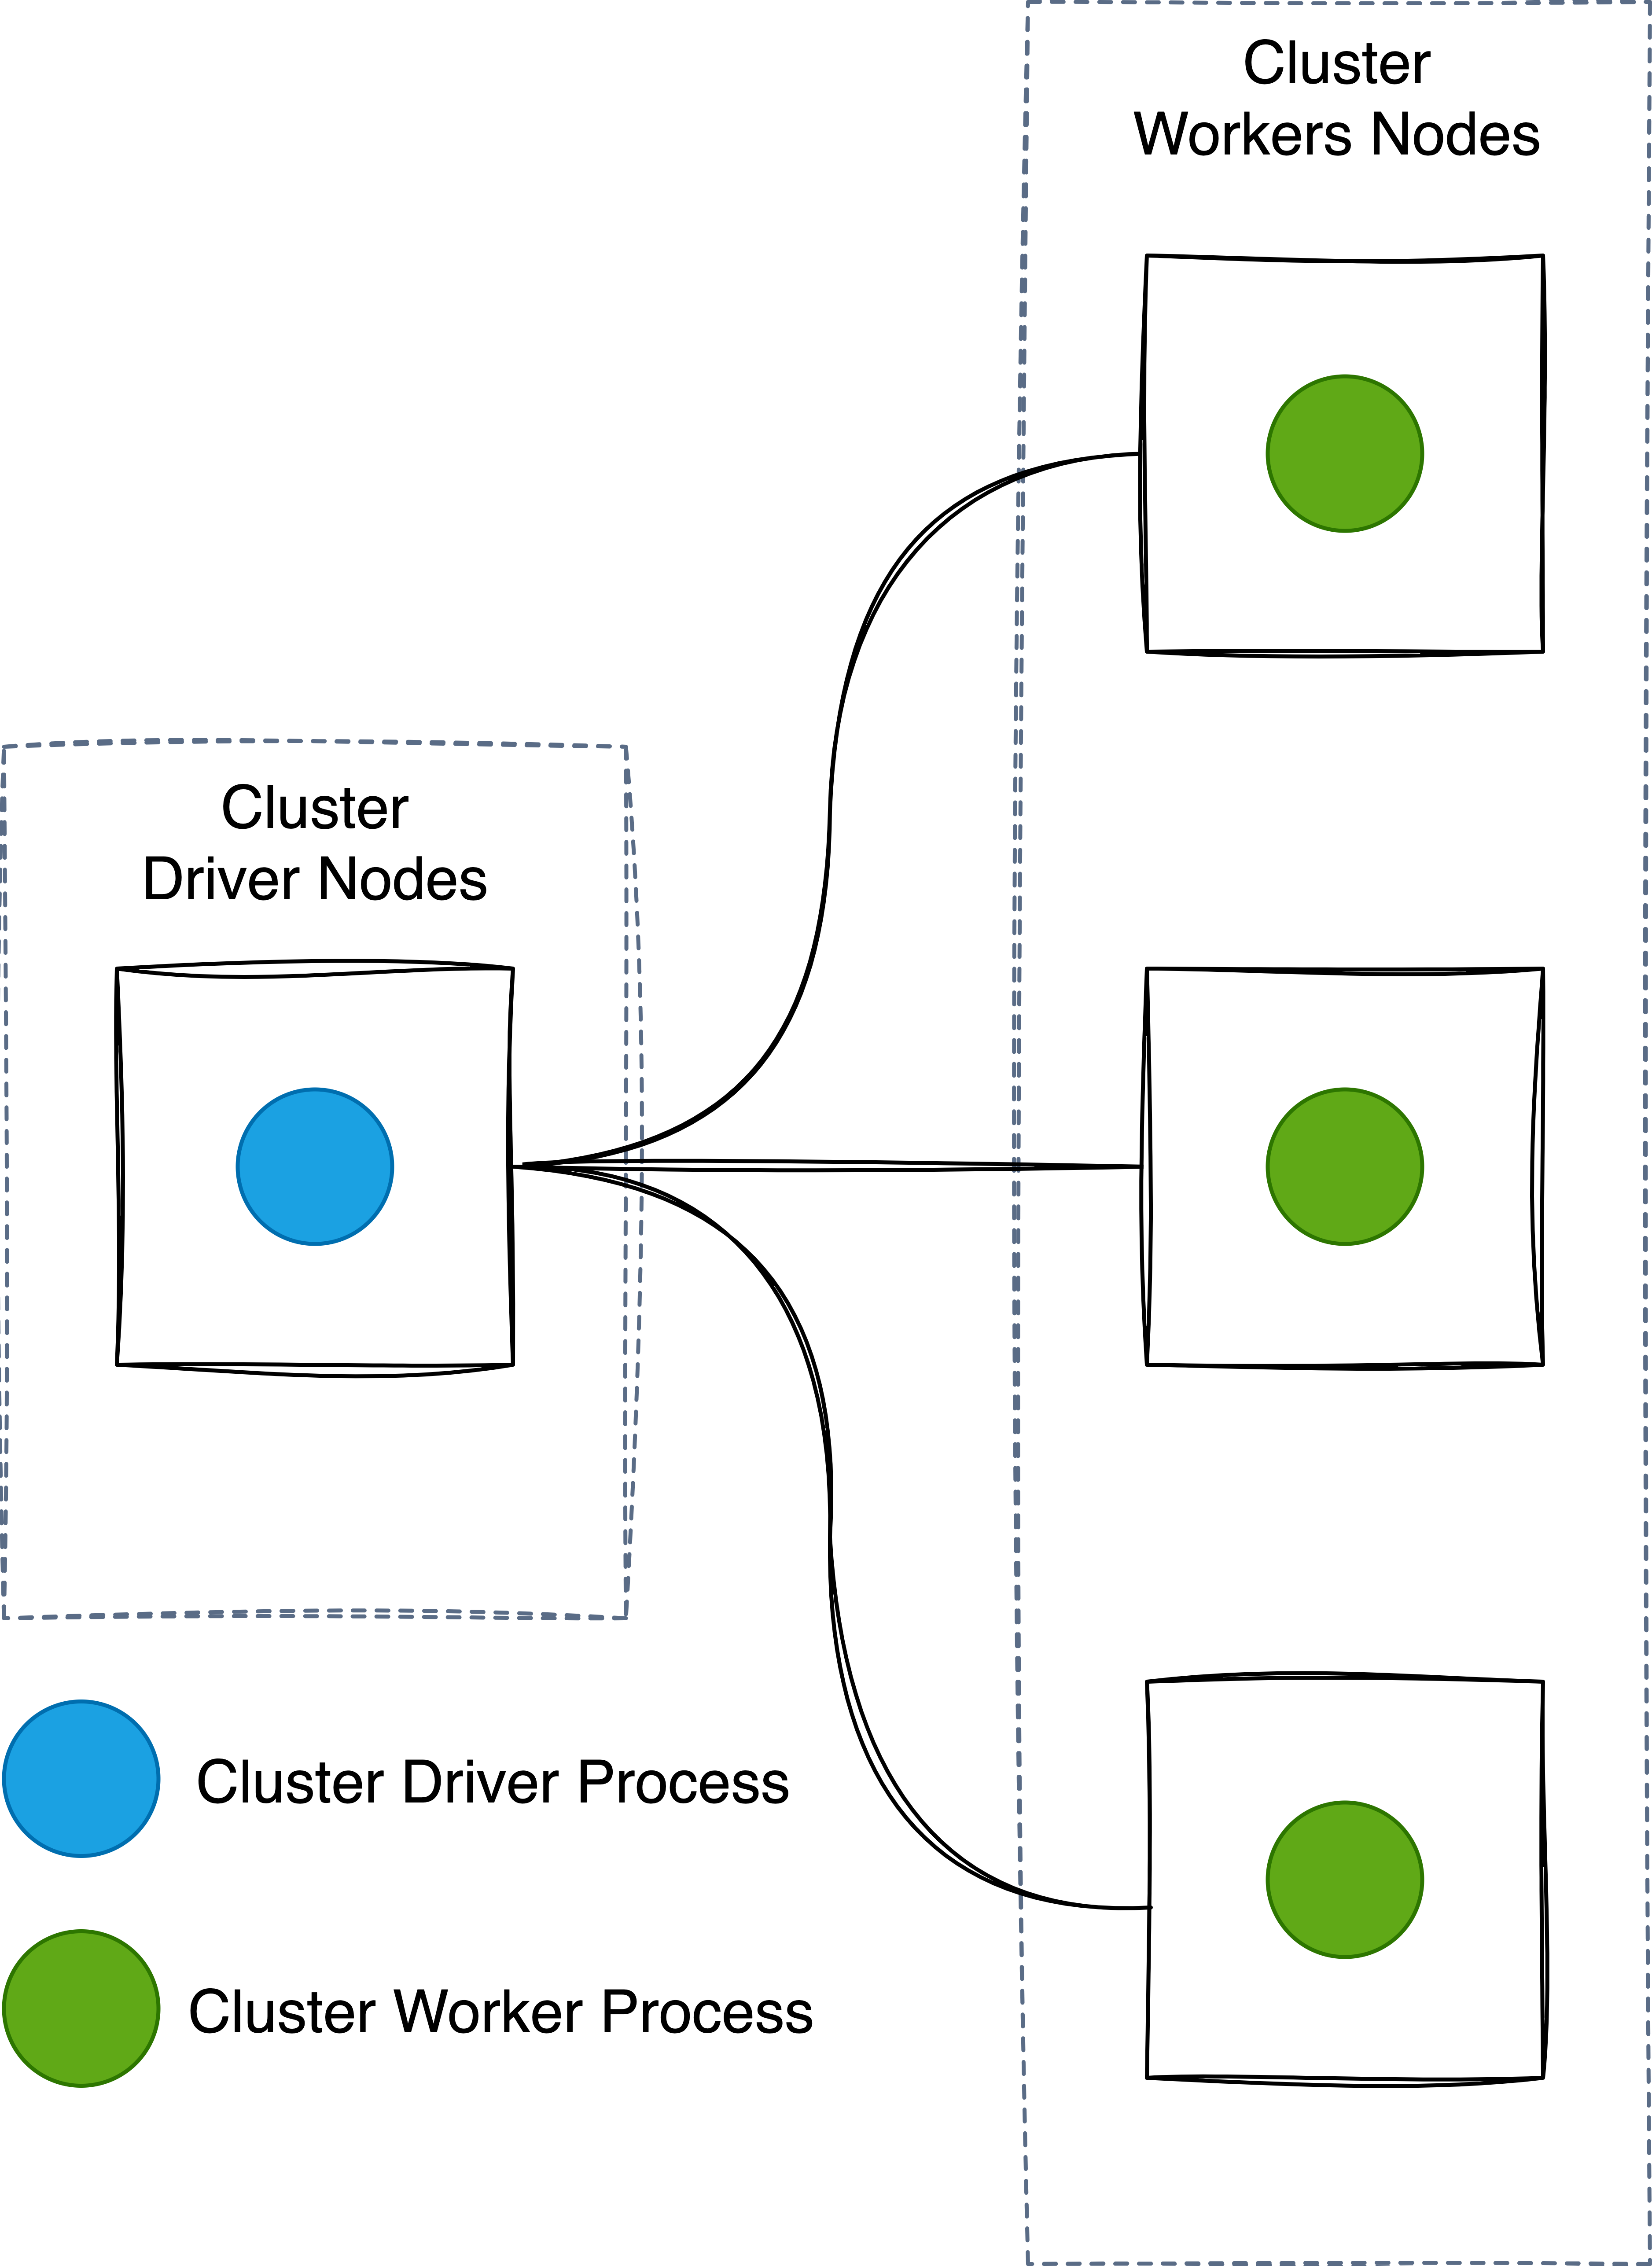
\includegraphics[width=\textwidth,height=.7\textheight,keepaspectratio]{./Figures/chapter-04/cluster_manager_processes}
        \caption{A cluster driver and worker (no Spark Application yet).}
    \end{figure}
\end{frame}

\begin{frame}
    \frametitle{Cluster Mode}
    \begin{itemize}
        \item Most common mode for running Spark Applications.
        \item User submits a pre-compiled JAR, Python script, or R script to a cluster manager.
        \item The cluster manager then launches the driver process on a worker node inside the cluster.
        \item Executor processes also launched within the cluster.
        \item Cluster manager handles all Spark Application processes.
        \item This means that the cluster manager is responsible for maintaining all Spark Application–related processes.
    \end{itemize}
\end{frame}

\begin{frame}
    \frametitle{Spark Cluster Mode}
    \begin{figure}
        \includegraphics[width=\textwidth,height=.7\textheight,keepaspectratio]{./Figures/chapter-04/spark_cluster_mode}
        \caption{Spark’s cluster mode.}\label{fig:cluster_mode}
    \end{figure}
\end{frame}

\begin{frame}
    \frametitle{Client Mode}
    \begin{itemize}
        \item Similar to cluster mode, but the  \textbf{\texttt{Spark driver remains on the client
        machine that submitted the application}}.
        \item \textbf{Client machine} is responsible for maintaining the Spark driver process.
        \item \textbf{Cluster manager} maintains executor processes.
        \item Commonly used with gateway machines or edge nodes.
        \item The driver is running on a machine outside of the cluster but that the workers are located on machines in the cluster.
    \end{itemize}
\end{frame}

\begin{frame}
    \frametitle{Spark Client Mode}
    \begin{figure}
        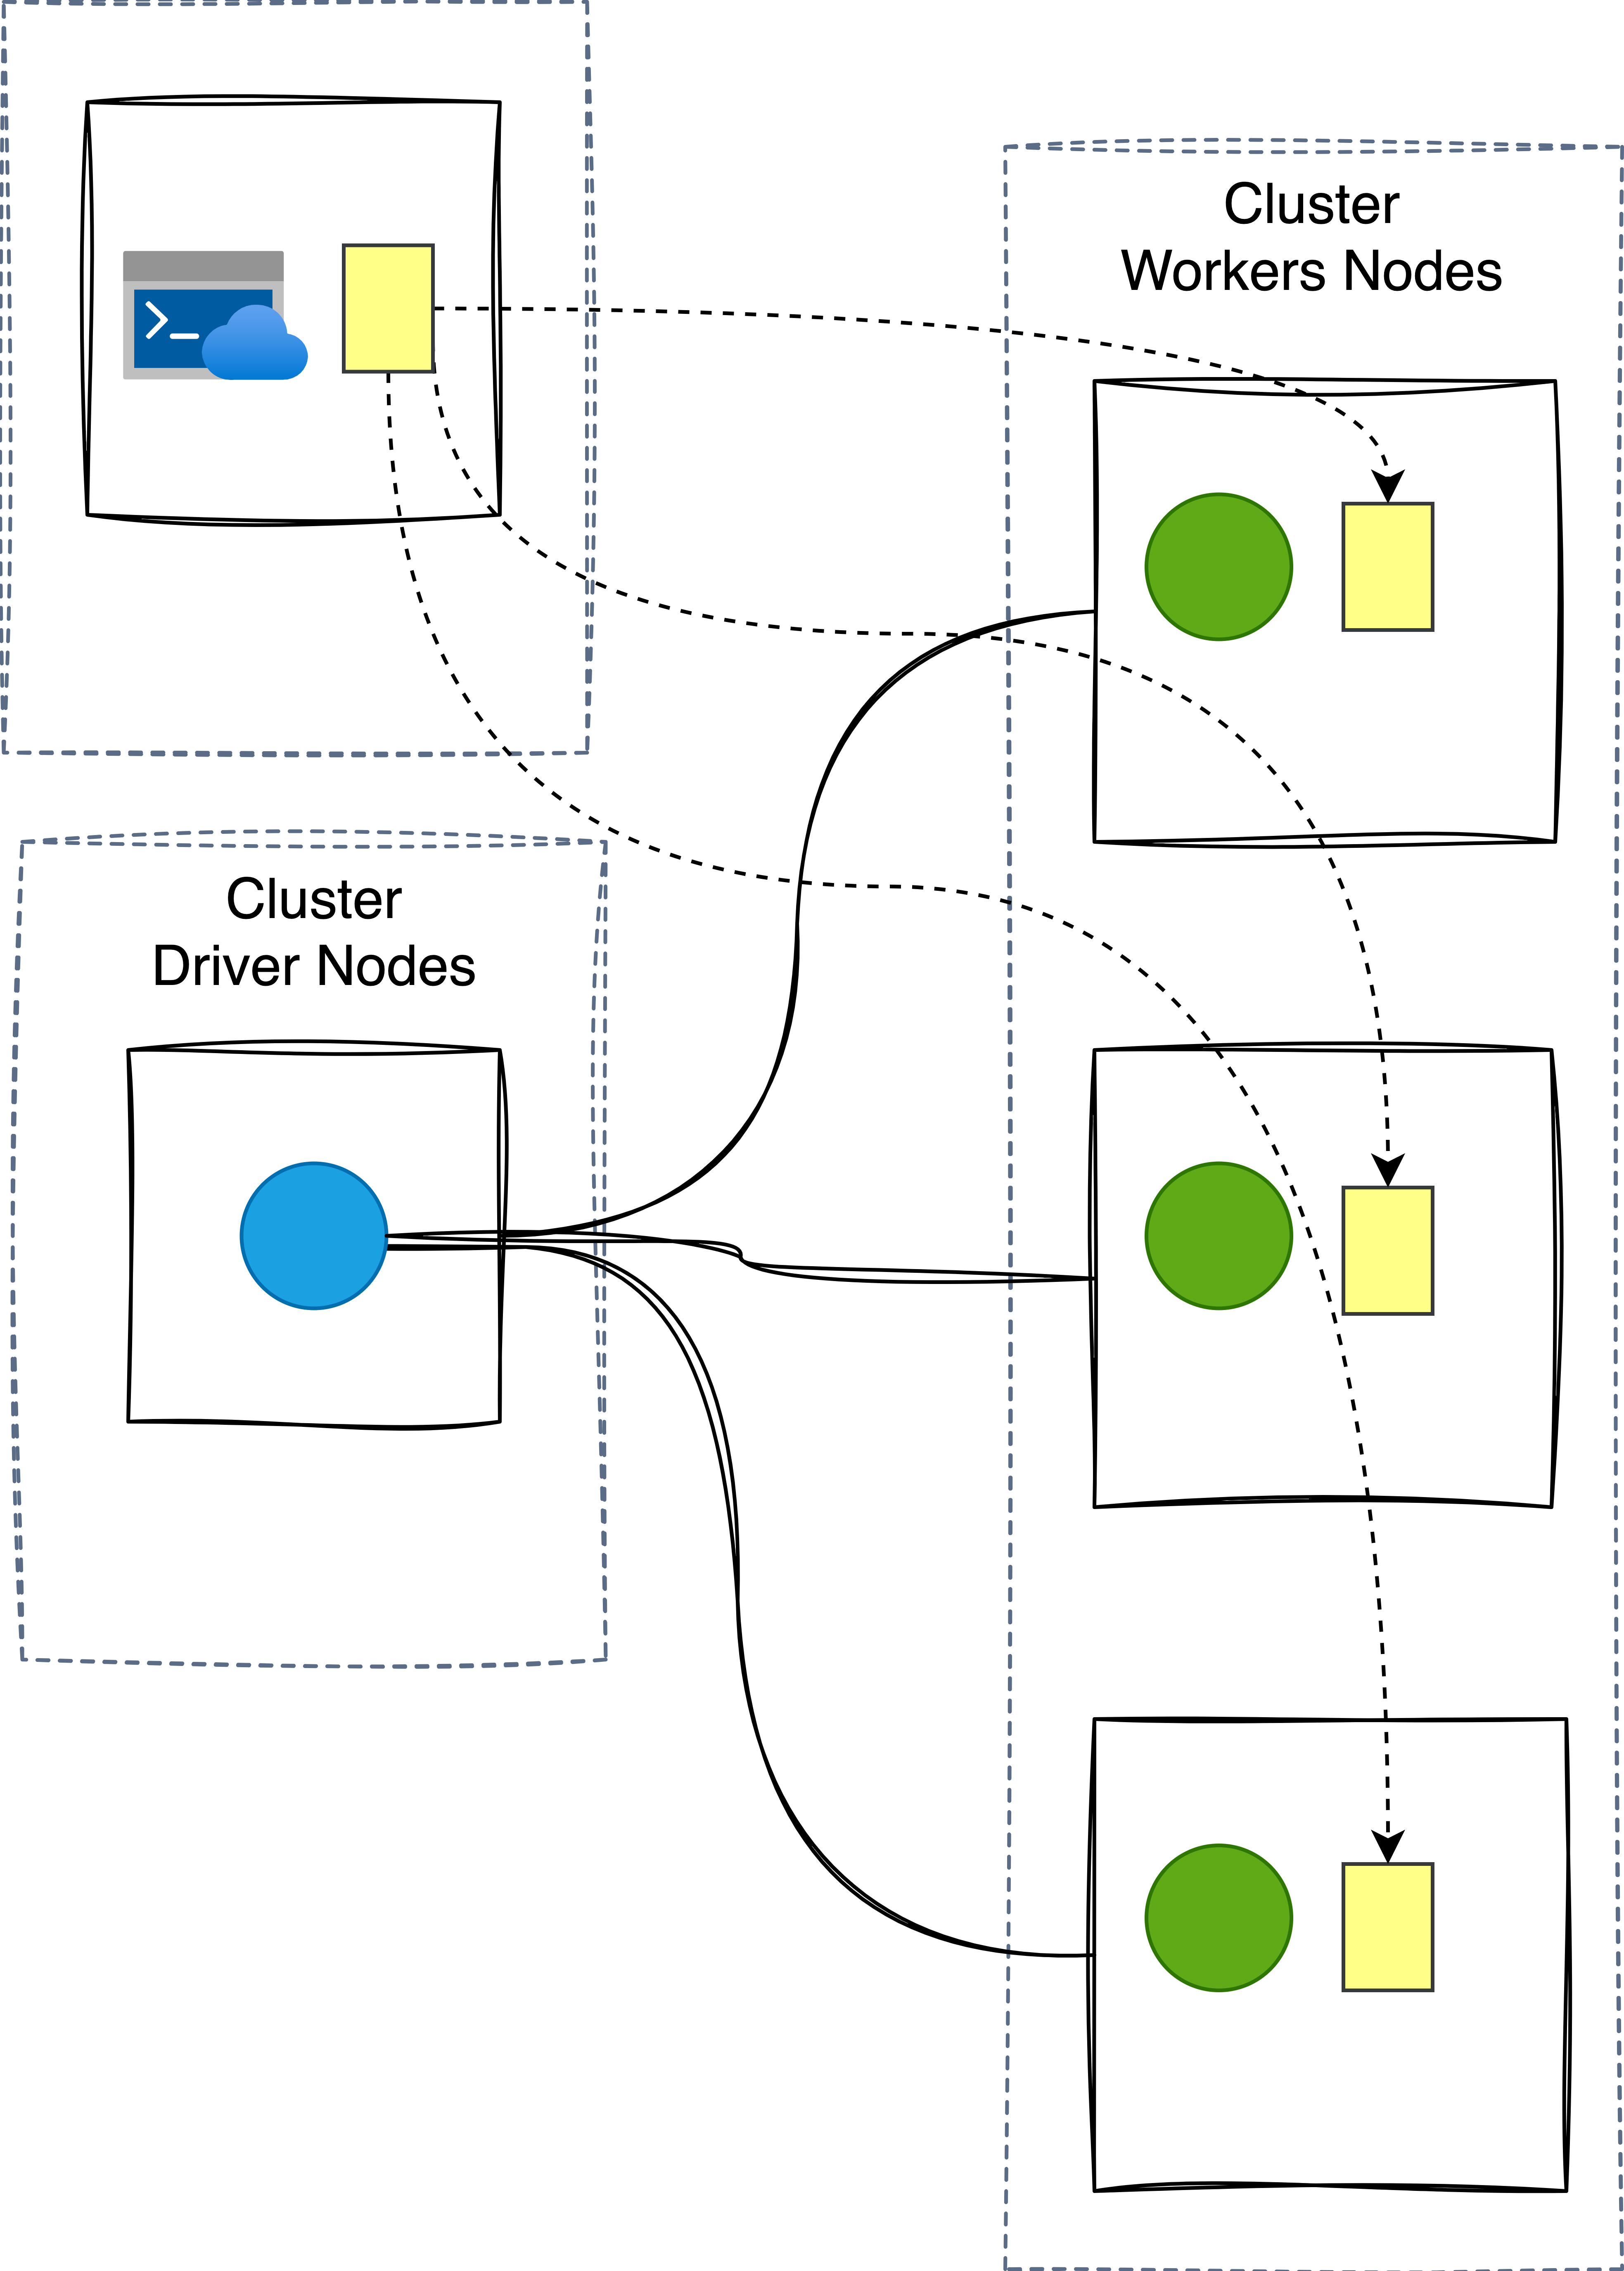
\includegraphics[width=\textwidth,height=.7\textheight,keepaspectratio]{./Figures/chapter-04/spark_client_mode}
        \caption{Spark’s client mode.}\label{fig:client_mode}
    \end{figure}
\end{frame}

\begin{frame}
    \frametitle{Local Mode}
    \begin{itemize}
        \item Runs the entire application on a single machine.
        \item Parallelism achieved through threads on the same machine.
        \item Ideal for learning, testing, or local development.
        \item Not recommended for production use.
    \end{itemize}
\end{frame}

%\begin{frame}
%    \frametitle{Spark Deployment Modes Cheat Sheet}
%    \begin{table}[h!]
%        \centering
%        \resizebox{\textwidth}{!}{%
%        \begin{tabular}{|p{2cm} |p{5cm} |p{5cm} |p{5cm}|}
%            \hline
%            \rowcolor{Gray}
%            \textbf{Mode} & \textbf{Driver} & \textbf{Executor} & \textbf{Cluster Manager} \\
%            \hline
%            \textbf{Local} & Runs on a single JVM & Runs with driver & Single host \\
%            \hline
%            \textbf{Standalone} & Any cluster node & Own JVM per node & Any host in cluster \\
%            \hline
%            \textbf{YARN (client)} & Client machine & NodeManager container & YARN Resource Manager \\
%            \hline
%            \textbf{YARN (cluster)} & YARN App Master & Similar to client & Similar to client \\
%            \hline
%            \textbf{Kubernetes} & Kubernetes pod & Individual pods & Kubernetes Master \\
%            \hline
%        \end{tabular}
%        }
%        \caption{Summary of Spark deployment modes}\label{tab:spark-deployment}
%    \end{table}
%\end{frame}
% Ch.04-18   | Spark Executors

\subsection{Spark executors}\label{subsec:spark-executors}

\begin{frame}
    \frametitle{Spark Executors in Depth}
    \begin{itemize}
        \item Executors are processes that run the tasks assigned by the driver.
        \item Each Spark Application has distinct executor processes.
        \item Typically, one executor runs per node in most deployment modes.
        \item Executors' main function: Execute tasks, return status, and communicate outcomes.
    \end{itemize}
\end{frame}

% Ch.04-19   | Spark Data Partitioning

\subsection{Data partition}\label{subsec:data-partition}


% Slide 1
\begin{frame}{Introduction to Data Distribution and Partitions}
    \begin{itemize}
        \item \textbf{Data Distribution:} Physical data is distributed across storage as partitions residing in either HDFS or cloud storage.
        \item \textbf{Data Abstraction:} Spark treats each partition as a high-level logical data abstraction—as a DataFrame in memory.
    \end{itemize}
\end{frame}

% Slide 2
\begin{frame}{Data Locality and Task Allocation}
    \begin{itemize}
        \item \textbf{Data Locality:} Each Spark executor is preferably allocated a task that requires it to read the partition closest to it in the network, observing data locality.
        \item \textbf{Optimal Task Allocation:} Partitioning allows for efficient parallelism.
        \item \textbf{Minimize Network Bandwidth:} A distributed scheme of breaking up data into chunks or partitions allows Spark executors to process only data that is close to them, minimizing network bandwidth.
    \end{itemize}
\end{frame}

% Slide 3
\begin{frame}{Benefits of Partitioning}
    \begin{itemize}
        \item \textbf{Efficient Parallelism:} Partitioning allows executors to process data close to them.
        \item \textbf{Dedicated Processing:} Each core on an executor works on its own partition, minimizing network bandwidth usage.
    \end{itemize}
\end{frame}

% Slide 4
\begin{frame}[fragile]{Practical Example - Distributing Data}
    \begin{lstlisting}[language=Python,label={lst:pyspark-data-partitioning}]
        log_df = spark.read.text("path_to_large_text_file").repartition(8)
        print(log_df.rdd.getNumPartitions())
    \end{lstlisting}
    This example splits data across clusters into eight partitions.
\end{frame}

% Slide 5
\begin{frame}[fragile]{Practical Example - Creating a DataFrame}
    \begin{lstlisting}[language=Python,label={lst:pyspark-creating-dataframe}]
        df = spark.range(0, 10000, 1, 8)
        print(df.rdd.getNumPartitions())
    \end{lstlisting}
    This creates a DataFrame of 10,000 integers over eight partitions in memory.
\end{frame}

% Slide 6
\begin{frame}{Conclusion}
    \begin{itemize}
        \item \textbf{Key Takeaway:} Efficient data partitioning is crucial for optimizing processing in Spark.
    \end{itemize}
\end{frame}

% Ch.04-20   | Spark Operations

\subsection{Spark Operations}\label{subsec:spark-operations}
\begin{frame}
    \frametitle{Spark Operations}
    \begin{itemize}
        \item Spark \textbf{operations} on distributed data can be classified into two types: transformations
        and actions.
        \item All spark operations are \texttt{\color{blue}{immutable}}.
    \end{itemize}
\end{frame}
\begin{frame}
    \frametitle{Immutable Objects}
    \begin{itemize}
        \item An object whose state cannot change after it has been constructed is
        called immutable (unchangable).\footnote{Referenced from https://otfried.org/courses/cs109scala/tutorial_mutable.html}
        \item  The methods of an immutable object do not modify the state of the object.
    \end{itemize}
\end{frame}

\begin{frame}
    \frametitle{Immutable Objects}
    \begin{figure}
        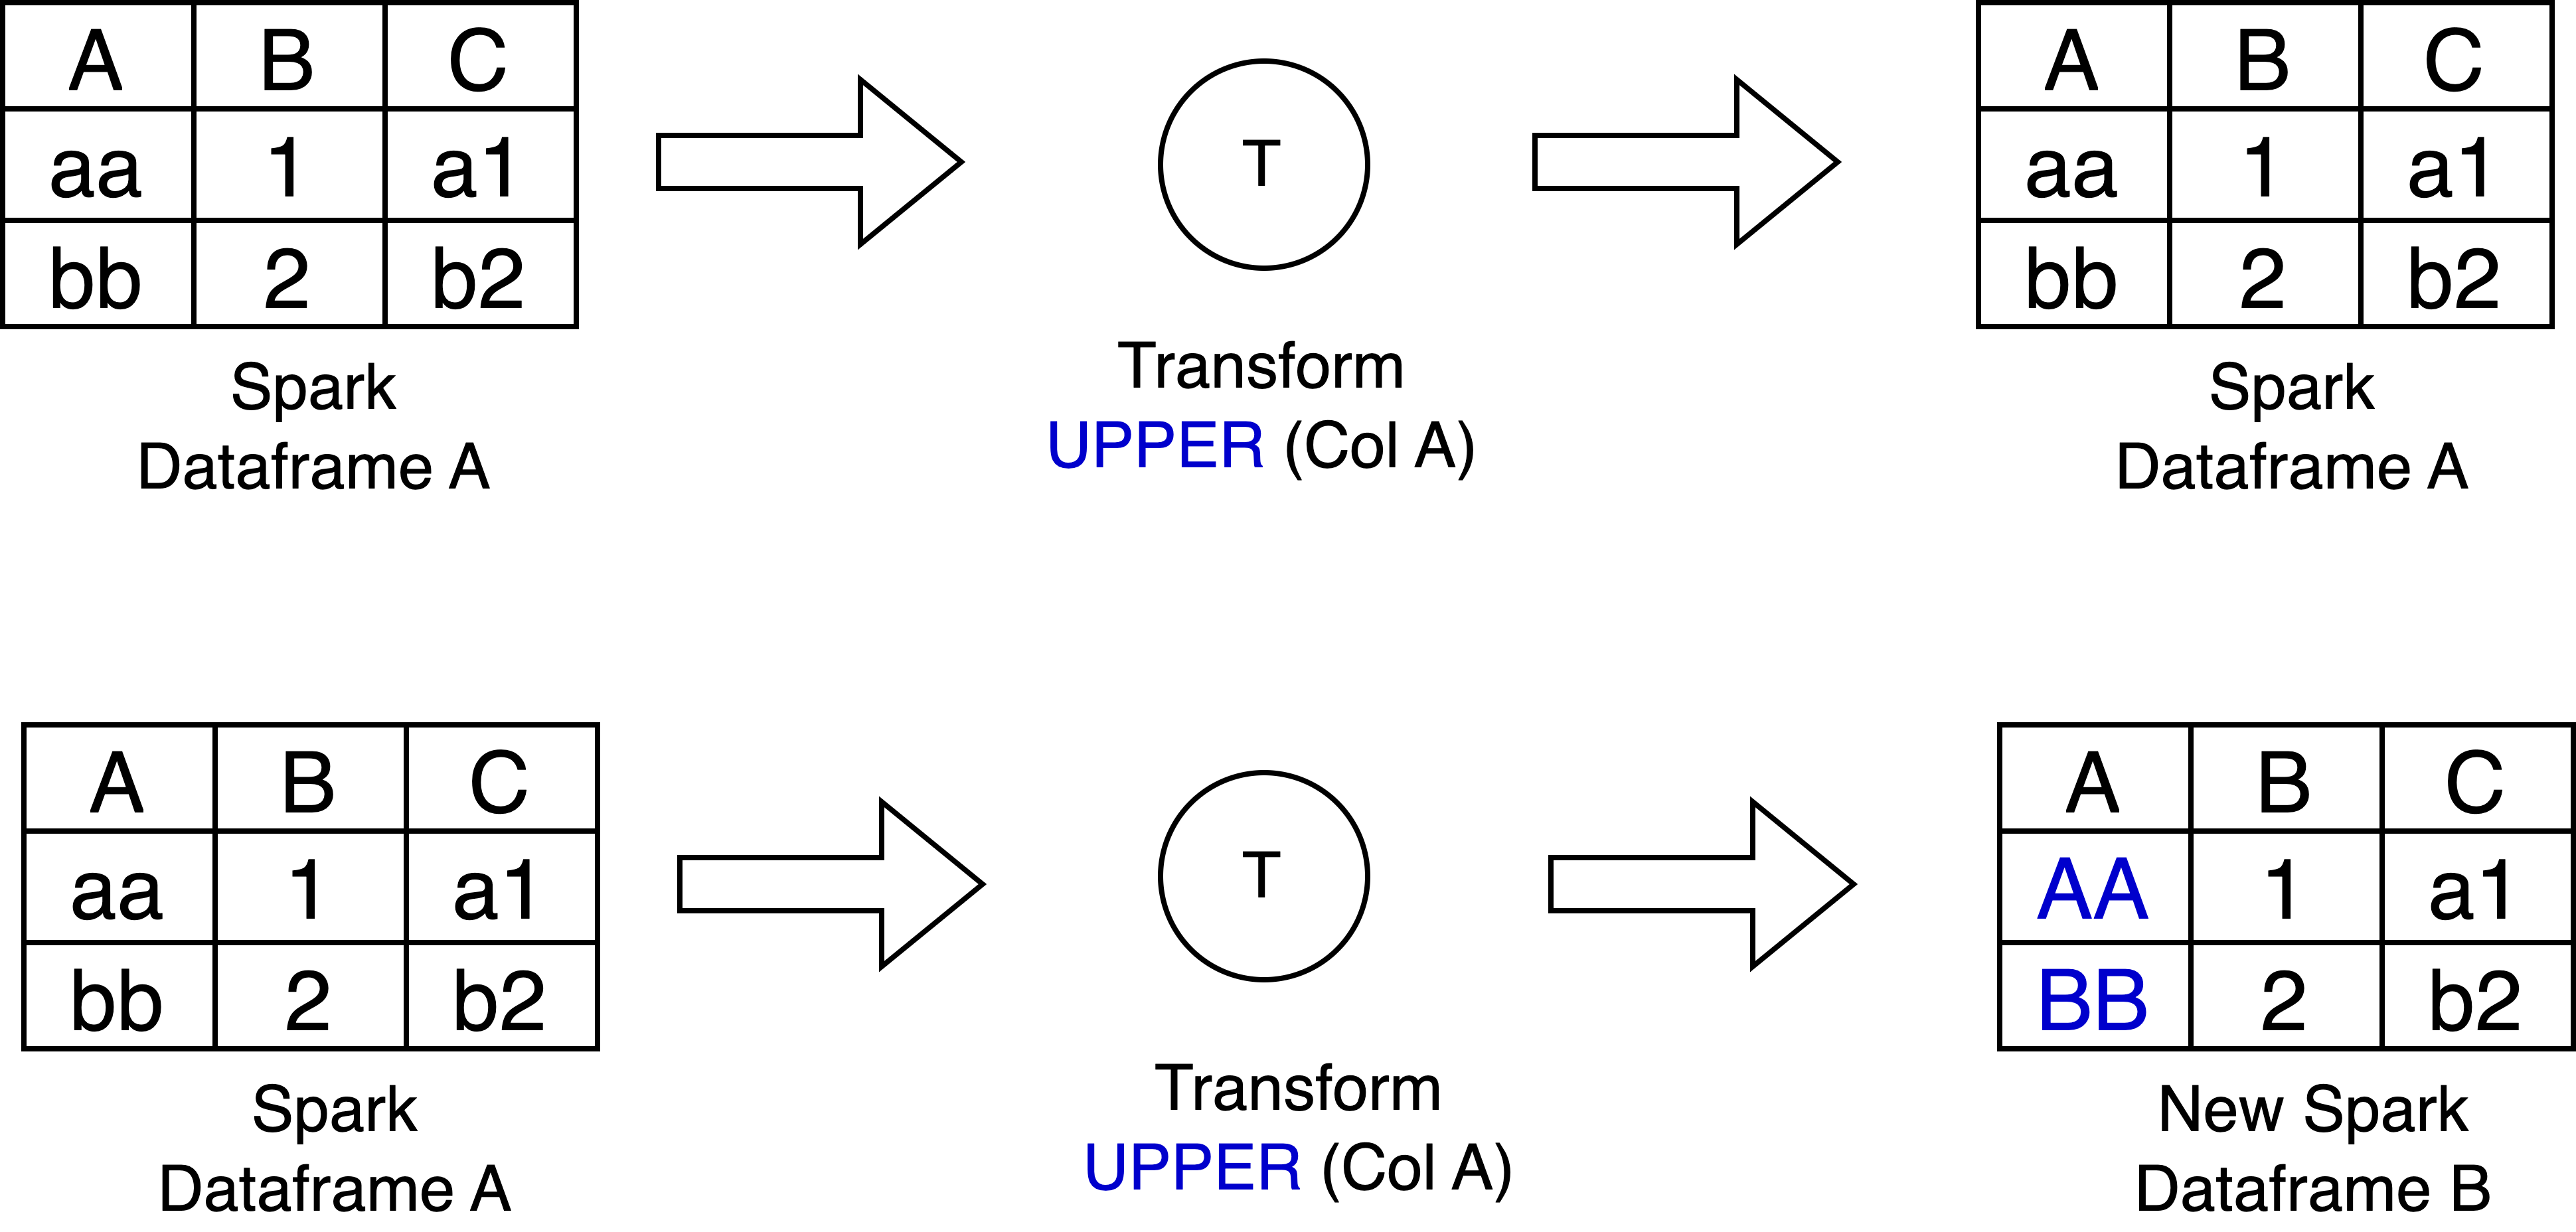
\includegraphics[width=\textwidth,height=.7\textheight,keepaspectratio]{./Figures/chapter-04/Immutable_df}
        \caption{Spark Dataframe is immutable, and you can't change its values.}\label{fig:Immutable_df}
    \end{figure}
\end{frame}

\begin{frame}[fragile]
    \frametitle{Immutable Objects}
    \begin{figure}
        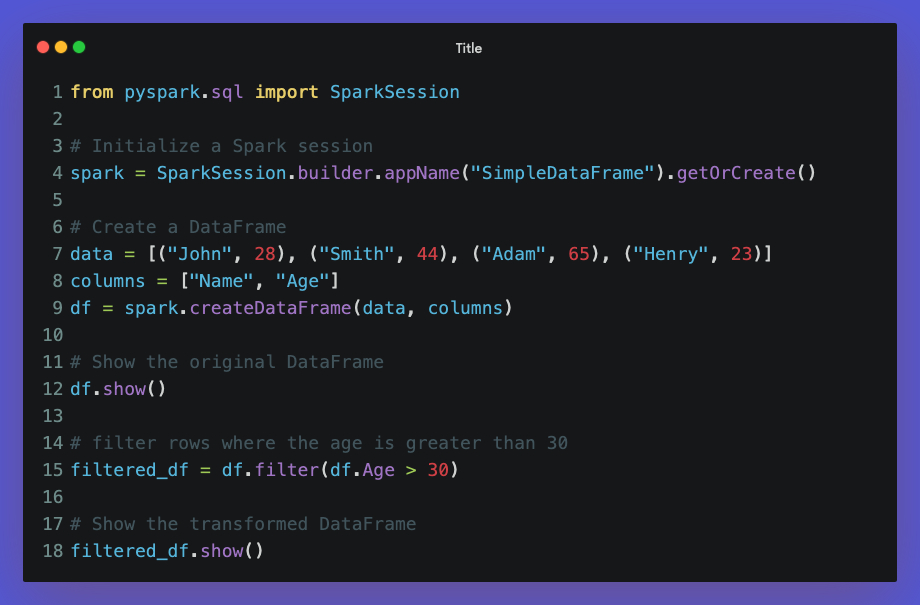
\includegraphics[width=\textwidth,height=.75\textheight,keepaspectratio]{./Figures/chapter-04/pyspark_immutable_df}
        \caption{Filtering a PySpark DataFrame Based on Age}\label{fig:pyspark_immutable_df}
    \end{figure}
\end{frame}
\begin{frame}[fragile]
    \frametitle{DEMO}
    DEMO
\end{frame}
\begin{frame}
    \frametitle{Spark Operations: Transformations}
    \begin{itemize}
        \item Transformations: transform a Spark DataFrame into a new DataFrame \textit{\color{blue}{without altering the original data}}.
        \item Example of Spark transformations, \texttt{\color{orange}{map(), select(), filter(), or drop()} }
    \end{itemize}
\end{frame}

\begin{frame}
    \frametitle{Spark Transformations: What are Lazy Transformations?}
    \begin{itemize}
        \item In Spark, transformations are \textit{lazy}.
        \item This means computations are not executed immediately.
        \item Spark builds a \textbf{DAG} (Directed Acyclic Graph) of transformations.
        \item All Transformations results are not computed immediately, but they are recorded or remembered as a \textbf{lineage}.
    \end{itemize}
\end{frame}

\begin{frame}
    \frametitle{Spark Transformations: Benefits of Lazy Evaluation}
    \begin{itemize}
        \item \textbf{Optimization:} A lineage allows Spark, at a later time in its execution plan, to rearrange certain transformations, coalesce
        them, or optimize transformations into stages for more efficient execution.
        \item \textbf{Resource Management:} Executes tasks efficiently, using fewer resources.
        \item \textbf{Fault Tolerance:} Easier to recompute parts of the pipeline if a part fails.
    \end{itemize}
\end{frame}

\begin{frame}
    \frametitle{Spark Transformations: Lazy Transformation}
    \begin{itemize}
        \item Consider a dataset with map and filter transformations.
        \item Spark does not execute these transformations when they are defined.
        \item Transformations are executed when an action (like \textbf{collect}, \textbf{count}) is called.
    \end{itemize}
\end{frame}
\begin{frame}
    \frametitle{Lazy Transformations Example}
    \begin{figure}
        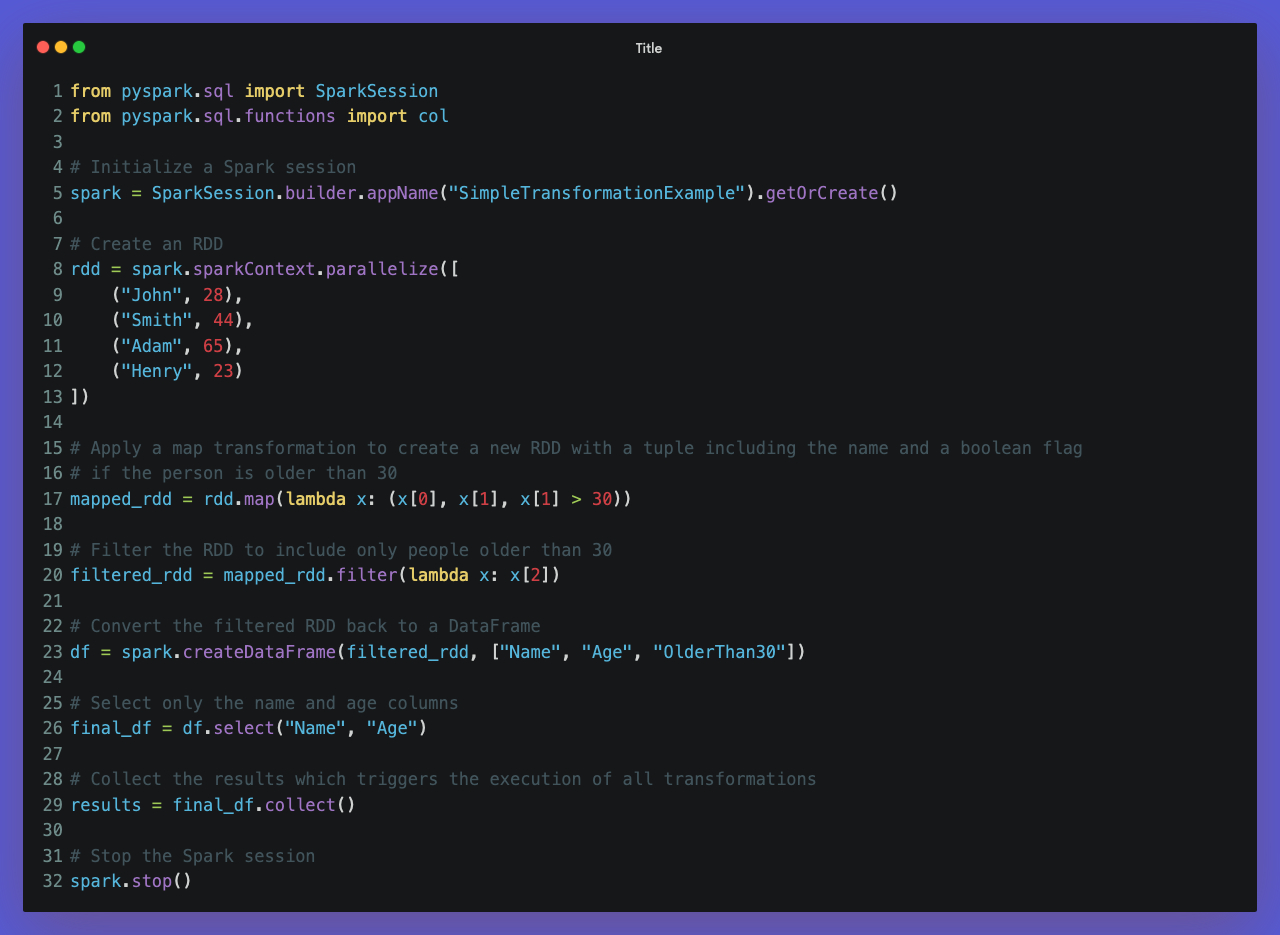
\includegraphics[width=\textwidth,height=.75\textheight,keepaspectratio]{./Figures/chapter-04/pyspark_transformations}
        \caption{Spark Lazy Transformations Example.}\label{fig:pyspark_transformations}
    \end{figure}
\end{frame}
\begin{frame}
    \frametitle{Spark Operations: Actions}
    \begin{itemize}
        \item An action triggers the lazy evaluation of all the recorded transformations.
        \item Actions are operations that trigger execution of transformations.
        \item They are used to either compute a result to be returned to the Spark driver program or to write data to an external storage system.
        \item Actions include operations like \textbf{count}, \textbf{collect}, \textbf{saveAsTextFile}, and \textbf{take}.
    \end{itemize}
\end{frame}

\begin{frame}
    \frametitle{Examples of Spark Actions}
    \begin{itemize}
        \item \textbf{collect()}: Collects all elements from the Spark context to the driver program.
        \item \textbf{count()}: Returns the number of elements in the dataset.
        \item \textbf{saveAsTextFile(path)}: Saves the dataset to a text file at the specified path.
        \item \textbf{take(n)}: Returns an array with the first n elements of the dataset.
    \end{itemize}
\end{frame}

% Ch.04-21   | Transformations Narrow Vs Wide

\subsection{Narrow and Wide Transformations}\label{subsec:narrow-and-wide-transformations}
\begin{frame}
    \frametitle{Introduction to Spark Transformations}
    \begin{itemize}
        \item Transformations create new RDDs from existing ones.
        \item Spark has two types of transformations: Narrow and Wide.
    \end{itemize}
\end{frame}

\begin{frame}
    \frametitle{What are Narrow Transformations?}
    \begin{itemize}
        \item Transformations that do not require data shuffling between partitions.
        \item Examples: \texttt{map()}, \texttt{filter()}.
        \item Data processing is limited to a single partition.
    \end{itemize}
\end{frame}

\begin{frame}
    \frametitle{What are Narrow Transformations?}
    \begin{figure}
        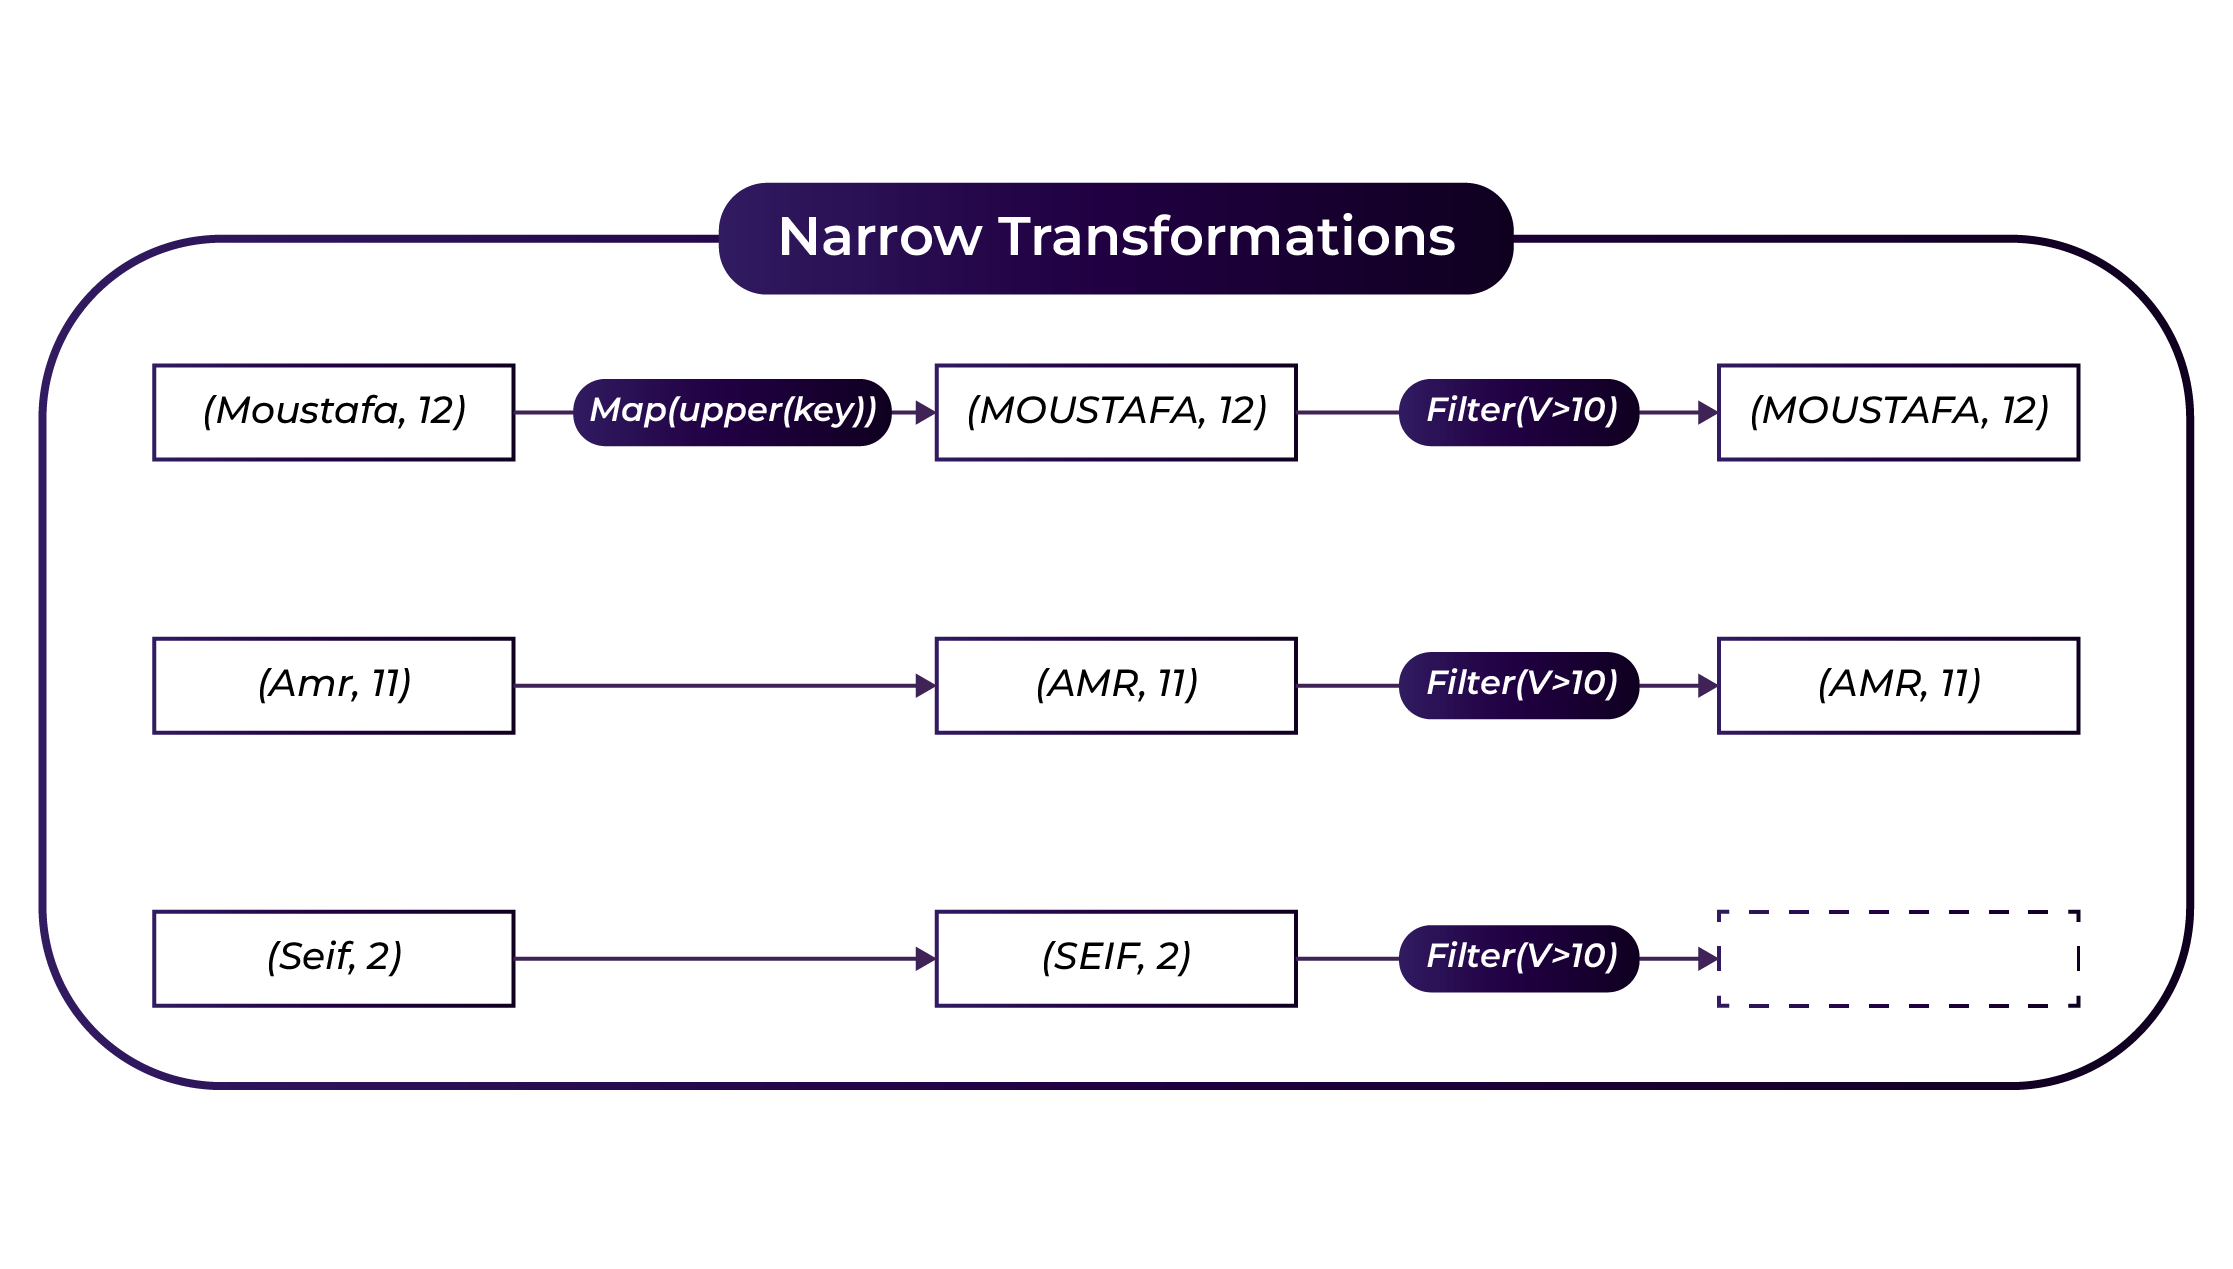
\includegraphics[width=\textwidth,height=.75\textheight,keepaspectratio]{./Figures/chapter-04/Narrow}
        \caption{Spark Narrow Transformations.}\label{fig:spark_narrow}
    \end{figure}
\end{frame}

\begin{frame}
    \frametitle{Benefits of Narrow Transformations}
    \begin{itemize}
        \item Efficient with minimal data movement.
        \item Best for independent data processing tasks.
    \end{itemize}
\end{frame}

\begin{frame}
    \frametitle{What are Wide Transformations?}
    \begin{itemize}
        \item Transformations that involve shuffling data across partitions.
        \item Examples: \texttt{groupBy()}, \texttt{reduceByKey()}.
    \end{itemize}
\end{frame}

\begin{frame}
    \frametitle{What are Wide Transformations?}
    \begin{figure}
        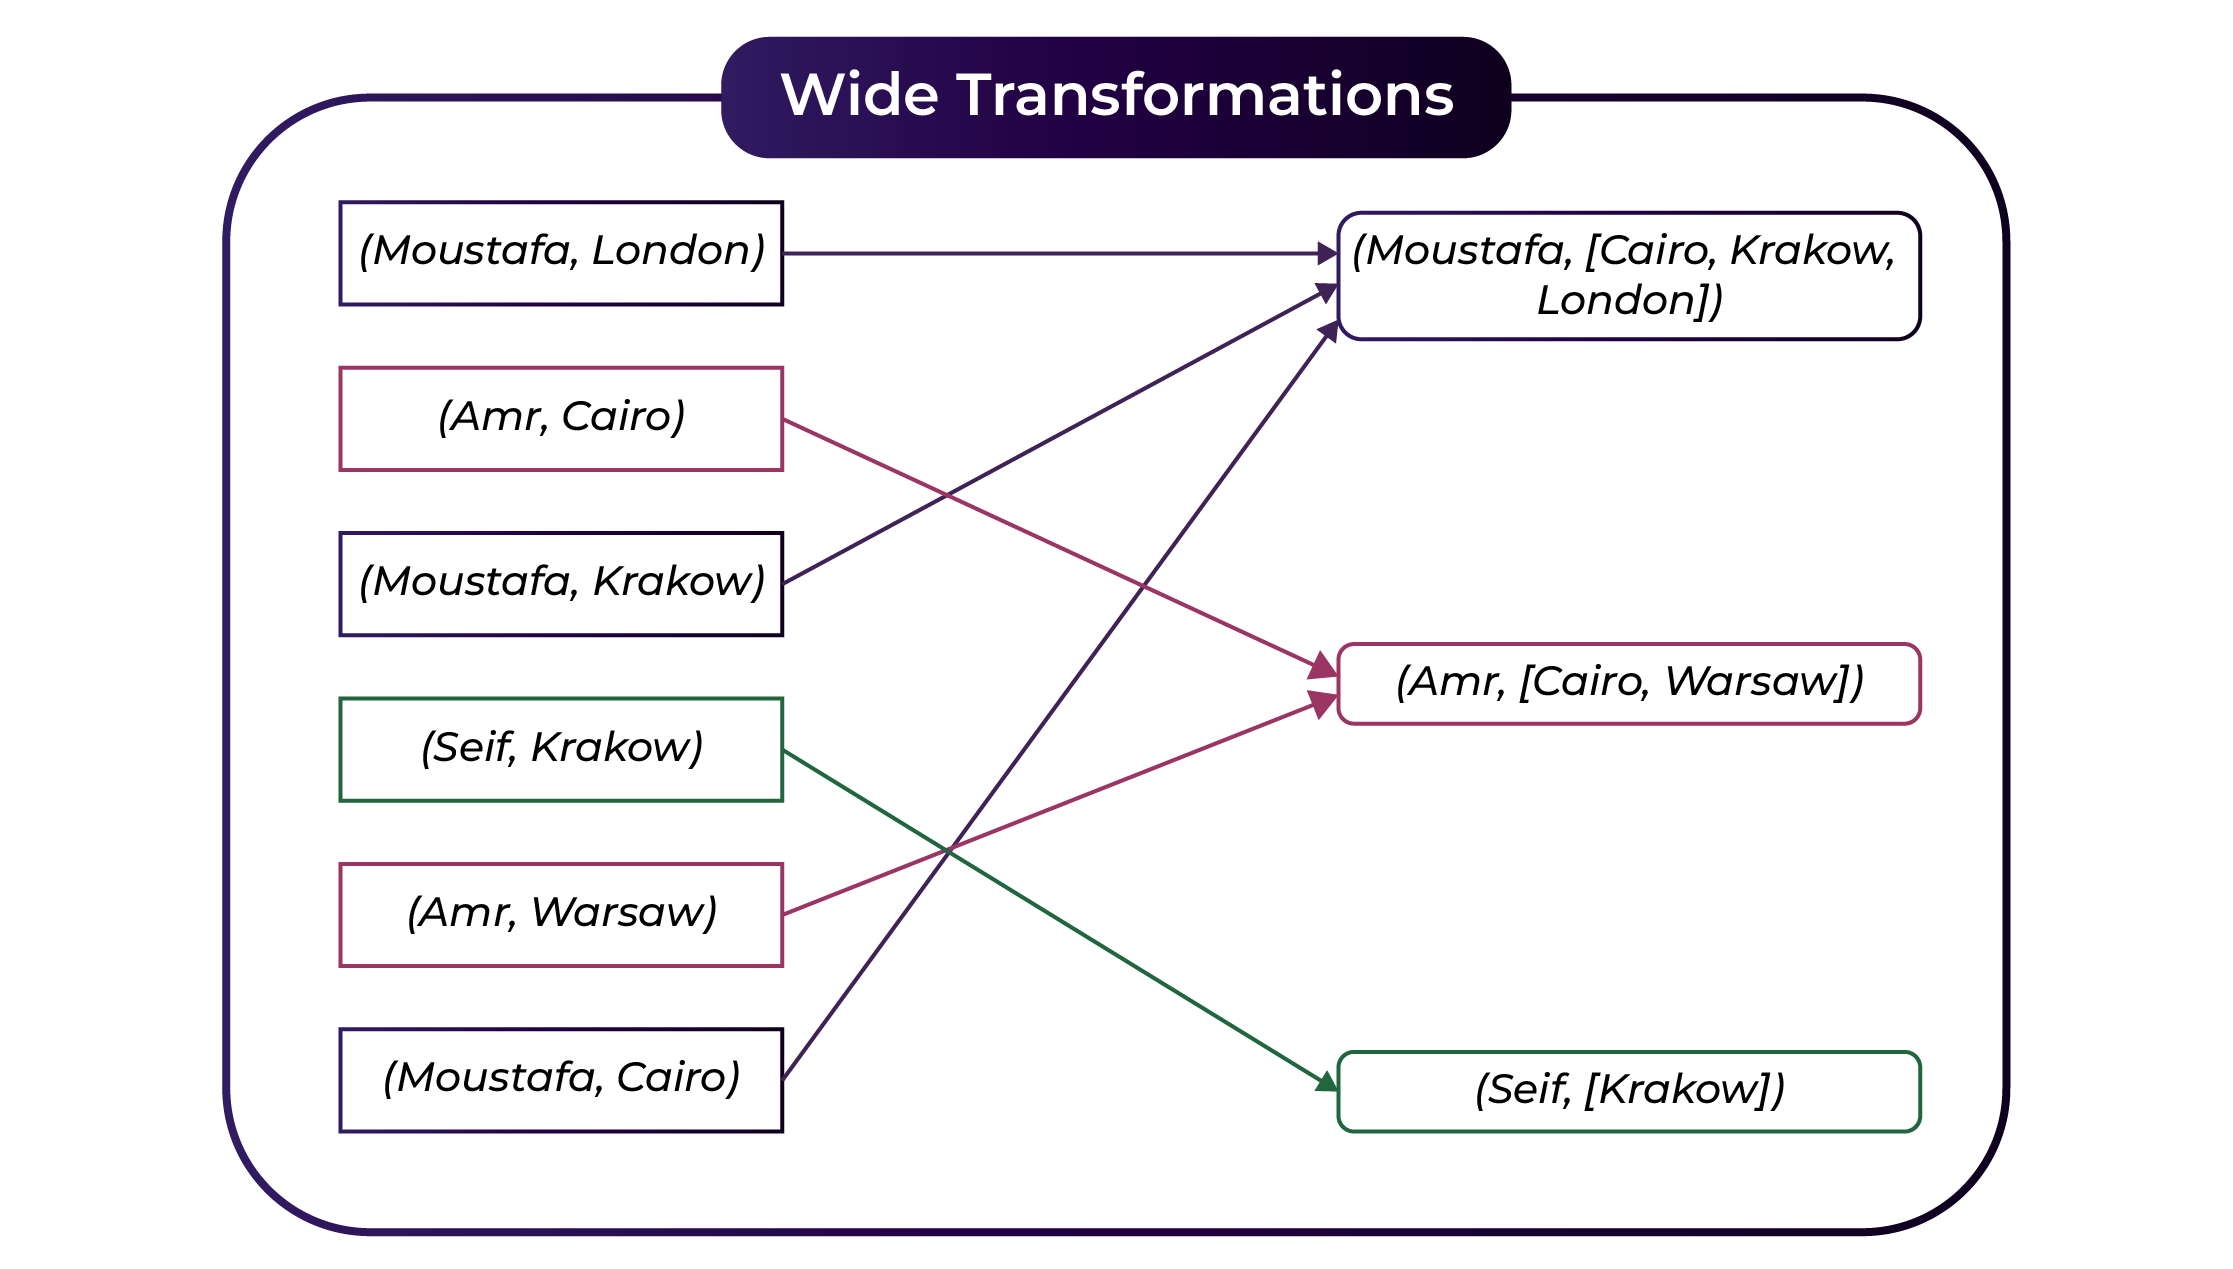
\includegraphics[width=\textwidth,height=.75\textheight,keepaspectratio]{./Figures/chapter-04/Wide}
        \caption{Spark Wide Transformations.}\label{fig:spark_wide}
    \end{figure}
\end{frame}

\begin{frame}
    \frametitle{Wide Transformations and Dependencies}
    \begin{itemize}
        \item \textbf{Wide Dependencies}: Require data from multiple partitions, often involving shuffling.
        \item \textbf{Examples}: \texttt{groupBy()}, \texttt{orderBy()} - data is combined across partitions, affecting performance.
        \item \textbf{Impact}: These transformations are necessary for operations like counting occurrences across a dataset.
    \end{itemize}
\end{frame}

\begin{frame}
    \frametitle{Implications of Wide Transformations}
    \begin{itemize}
        \item Shuffling can be expensive in terms of time and network I/O.
        \item Essential for aggregation and grouping operations.
    \end{itemize}
\end{frame}

\begin{frame}
    \frametitle{Narrow vs. Wide Dependencies}
    \begin{itemize}
        \item \textbf{Narrow Dependencies}: A single output partition can be computed from a single input partition without data exchange.
        \item \textbf{Examples}: \texttt{filter()}, \texttt{contains()} - operate independently on partitions.
    \end{itemize}
\end{frame}

\subsection{Repartition vs. Coalesce}\label{subsec:repartition-vs-coalesce}
\begin{frame}
    \frametitle{Repartition vs. Coalesce}
    \begin{itemize}
        \item In Apache Spark, repartition and coalesce are two methods used to change the number of partitions in an RDD (Resilient
        Distributed Dataset).
    \end{itemize}
\end{frame}

\begin{frame}
    \frametitle{Repartition vs. Coalesce}

    \begin{table}[h!]
        \centering
        \resizebox{\textwidth}{!}{%
            \begin{tabular}{|p{2cm} |p{6cm} |p{6cm} |}
                \hline
                \rowcolor{Gray}
                \hline
                \textbf{Aspect}    & \textbf{Repartition}                                                                                                & \textbf{Coalesce}                                                                                                         \\
                \hline
                \textbf{Purpose}   & \textcolor{blue}{Increases or decreases} the number of partitions. & \textcolor{blue}{Decreases} the number of partitions. \\
                \hline
                \textbf{Mechanism} & \textcolor{blue}{Shuffles all} the data across the network to create a new set of partitions. & \textcolor{blue}{Merges existing} partitions \textcolor{blue}{without} a full data shuffle. \\
                \hline
                \textbf{Use Case}  & Ideal for increasing the number of partitions or significantly \textcolor{blue}{changing the distribution} of data. & Efficient for \textcolor{blue}{reducing the number} of partitions when the target number is less than the current number. \\
                \hline
                \textbf{Cost}      & Expensive due to the \textcolor{blue}{full data shuffle}.                                                         & Less expensive than \texttt{repartition} as it \textcolor{blue}{minimizes data movement}.                               \\
                \hline
            \end{tabular}
        }
        \caption{Comparison of Repartition and Coalesce in Apache Spark}
    \end{table}
\end{frame}

\begin{frame}[fragile]
    \frametitle{High-Level Code: Repartition}
    \begin{lstlisting}[language=scala]
def repartition(numPartitions: Int)(implicit ord: Ordering[T] = null): RDD[T] = withScope {
  coalesce(numPartitions, shuffle = true)
}
    \end{lstlisting}
    \begin{itemize}
        \item \textbf{Key Points}:
        \begin{itemize}
            \item \textbf{Shuffle}: Always performs a shuffle by calling `coalesce` with `shuffle = true`.
            \item \textbf{Usage}: Suitable for both increasing and decreasing the number of partitions with even data distribution.
        \end{itemize}
    \end{itemize}
\end{frame}

\begin{frame}
    \frametitle{High-Level Code: Repartition}

        \begin{itemize}
            \item \textbf{Operation}: Calls `coalesce` with `shuffle = true`.
            \item \textbf{Process}: Full data shuffle across the network to redistribute data evenly.
            \item \textbf{Impact on Logs}:
            \begin{itemize}
                \item Increased log entries due to extensive shuffle operations.
                \item Higher overhead and cost.
                \item Useful for balancing load and increasing parallelism.
            \end{itemize}
        \end{itemize}
\end{frame}

\begin{frame}
    \frametitle{High-Level Code: Repartition}
    \begin{itemize}
        \item Shuffling Logic (If shuffle is true):

            \begin{itemize}
                \item Data is shuffled to distribute it evenly across the new partitions.
                \item Each item is assigned a new partition based on a random function.
                \item A new RDD is created with the shuffled data and the specified number of partitions.
            \end{itemize}
        \end{itemize}
\end{frame}




\begin{frame}[fragile]
    \frametitle{High-Level Code: Coalesce}

    \begin{lstlisting}[language=scala,basicstyle=\tiny]
def coalesce(numPartitions: Int, shuffle: Boolean = false,
             partitionCoalescer: Option[PartitionCoalescer] = Option.empty)
            (implicit ord: Ordering[T] = null): RDD[T] = withScope {
  require(numPartitions > 0, s"Number of partitions ($numPartitions) must be positive.")
  if (shuffle) {
    // Shuffle logic
    val distributePartition = (index: Int, items: Iterator[T]) => {
      var position = new XORShiftRandom(index).nextInt(numPartitions)
      items.map { t =>
        position = position + 1
        (position, t)
      }
    } : Iterator[(Int, T)]
    new CoalescedRDD(new ShuffledRDD[Int, T, T](
        mapPartitionsWithIndexInternal(distributePartition, isOrderSensitive = true),
        new HashPartitioner(numPartitions)),
      numPartitions,
      partitionCoalescer).values
  } else {
    // No-shuffle logic
    new CoalescedRDD(this, numPartitions, partitionCoalescer)
  }
}
    \end{lstlisting}

\end{frame}

\begin{frame}[fragile]
    \frametitle{High-Level Code: Coalesce}
    \begin{itemize}
        \item \textbf{Key Points}:
        \begin{itemize}
            \item \textbf{Shuffle}: Optional; can perform a shuffle if `shuffle = true`.
            \item \textbf{No Shuffle}: Default behavior (without shuffle) merges partitions locally.
            \item \textbf{Usage}: Efficient for reducing the number of partitions without shuffling.
        \end{itemize}
    \end{itemize}
\end{frame}




\begin{frame}
    \frametitle{High-Level Code: Coalesce}

    \begin{itemize}
        \begin{itemize}
            \item \textbf{Operation}: Can operate with or without shuffle.
            \item \textbf{Process}:
            \begin{itemize}
                \item \textbf{No Shuffle (default)}: Merges partitions locally.
                \item \textbf{With Shuffle}: Performs a shuffle for even data distribution if specified.
            \end{itemize}
            \item \textbf{Impact on Logs}:
            \begin{itemize}
                \item Decreased log entries when merging locally without shuffle.
                \item Lower overhead and cost.
                \item Efficient for reducing partitions, especially useful for write operations.
                \item Optional shuffle provides flexibility for balanced distribution.
            \end{itemize}
        \end{itemize}
    \end{itemize}
\end{frame}
%
%\begin{frame}
%\frametitle{Conclusion}
%
%This comparison illustrates that `repartition` always performs a shuffle to ensure even data distribution, which can be beneficial for load balancing but is more costly in terms of log entries and network overhead. In contrast, `coalesce` is more flexible and efficient for reducing the number of partitions without a shuffle, making it suitable for write operations with lower cost, while also allowing an optional shuffle for cases where balanced distribution is necessary.
%\end{frame}

\subsection{Understanding Spark Application Concepts}\label{subsec:understanding-spark-application-concepts}

\begin{frame}
    \frametitle{Understanding Spark Application Concepts}
    \begin{itemize}
        \item \textbf{Job}: A parallel computation consisting of multiple tasks that gets spawned in response
        to a Spark action (e.g., save(), collect()).
        \item \textbf{Stage}: Each job gets divided into smaller sets of tasks called stages that depend on each
        other.
        \item \textbf{Task}: A single unit of work or execution that will be sent to a Spark executor.
    \end{itemize}
\end{frame}
\begin{frame}
    \frametitle{Spark Jobs}
    \begin{figure}
        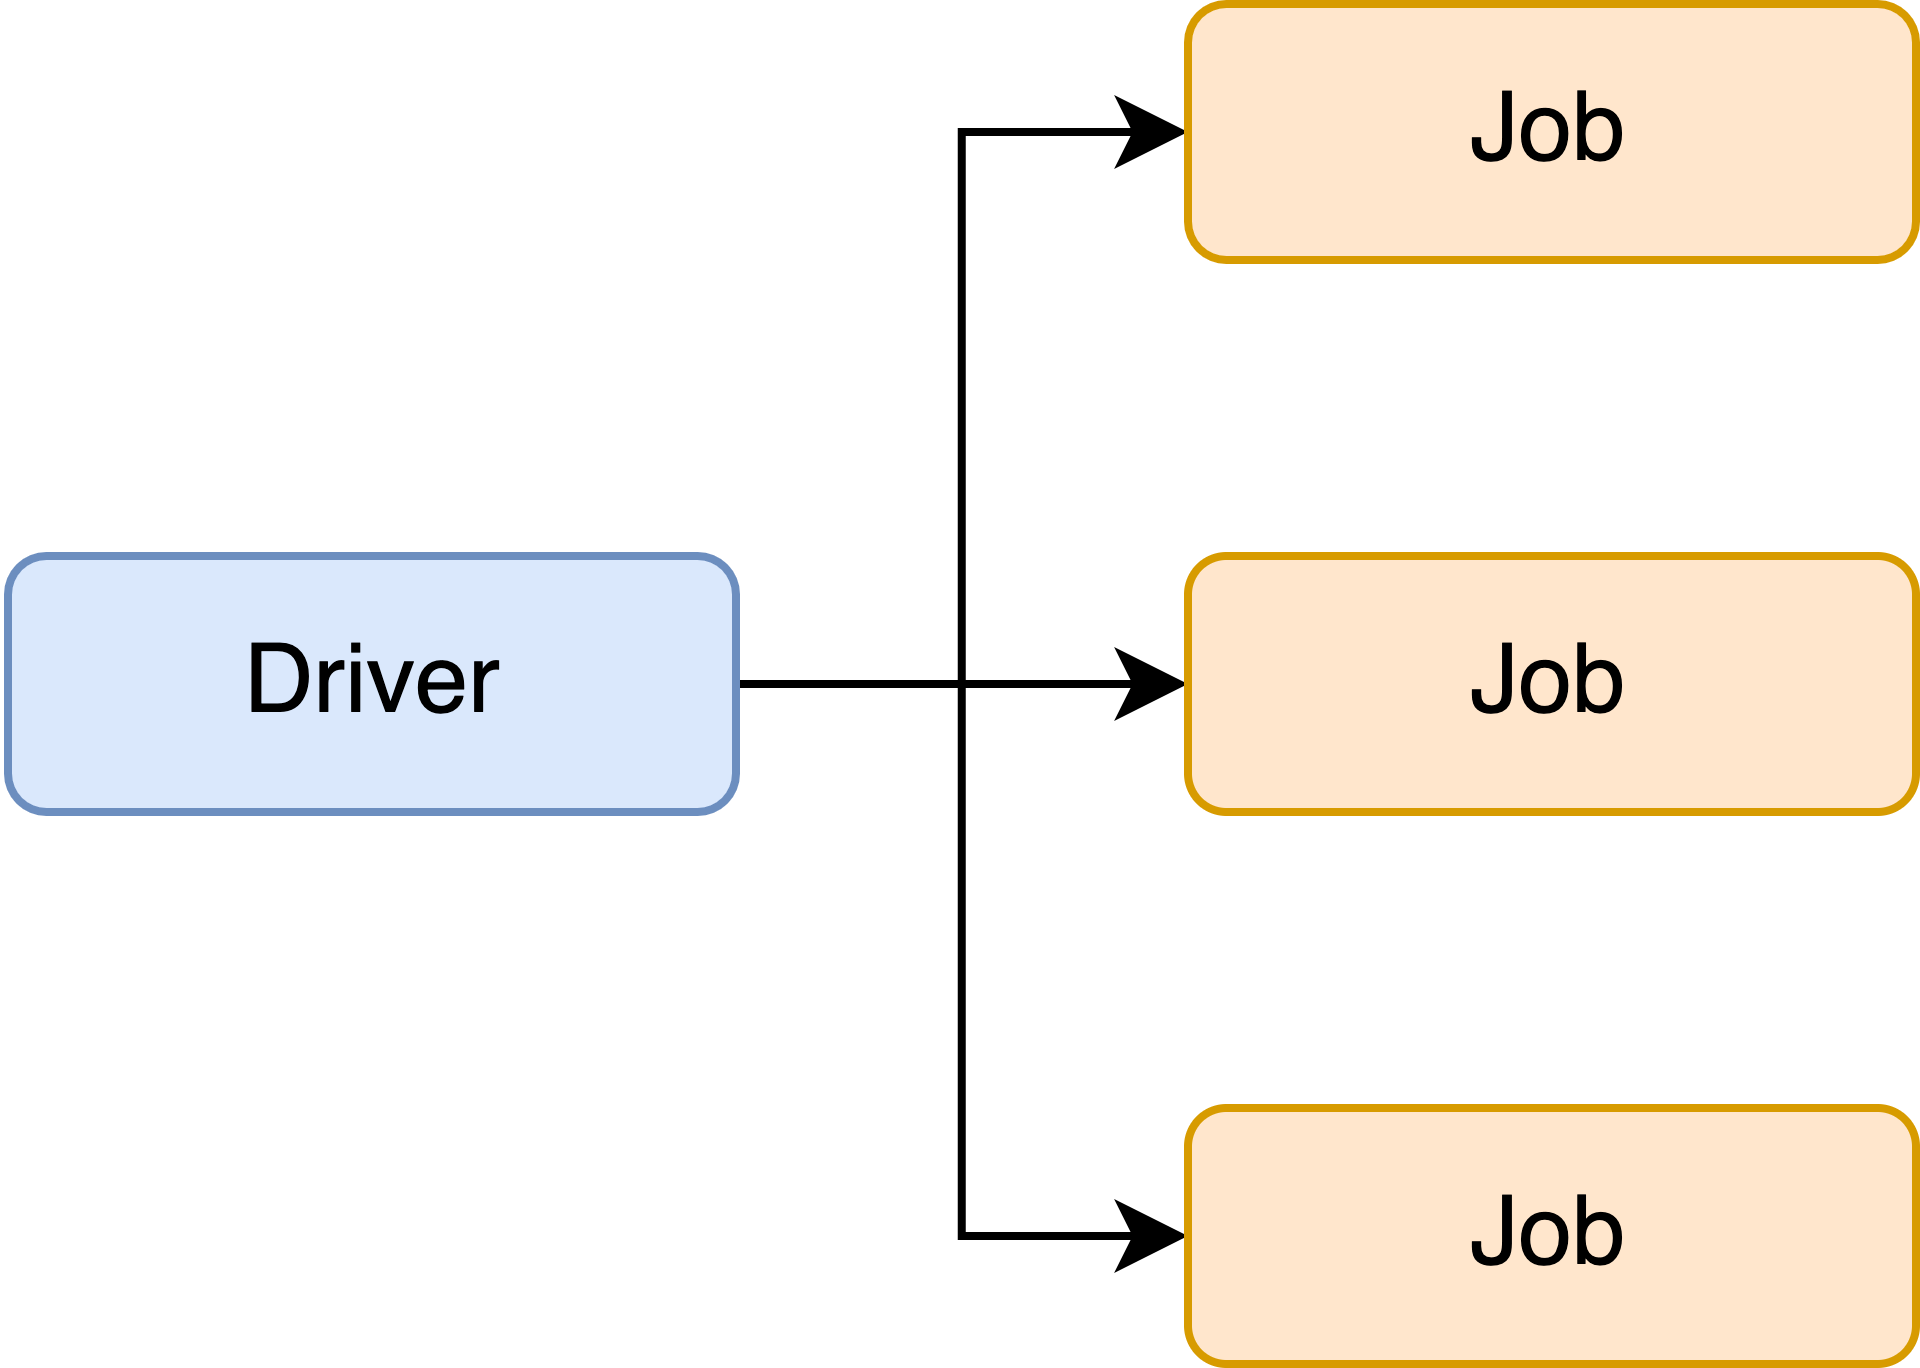
\includegraphics[width=\textwidth,height=.7\textheight,keepaspectratio]{./Figures/chapter-04/spark_job}
        \caption{Spark driver creating one or more Spark jobs.}\label{fig:spark_job}
    \end{figure}
\end{frame}
\begin{frame}
    \frametitle{Spark Stages}
    \begin{figure}
        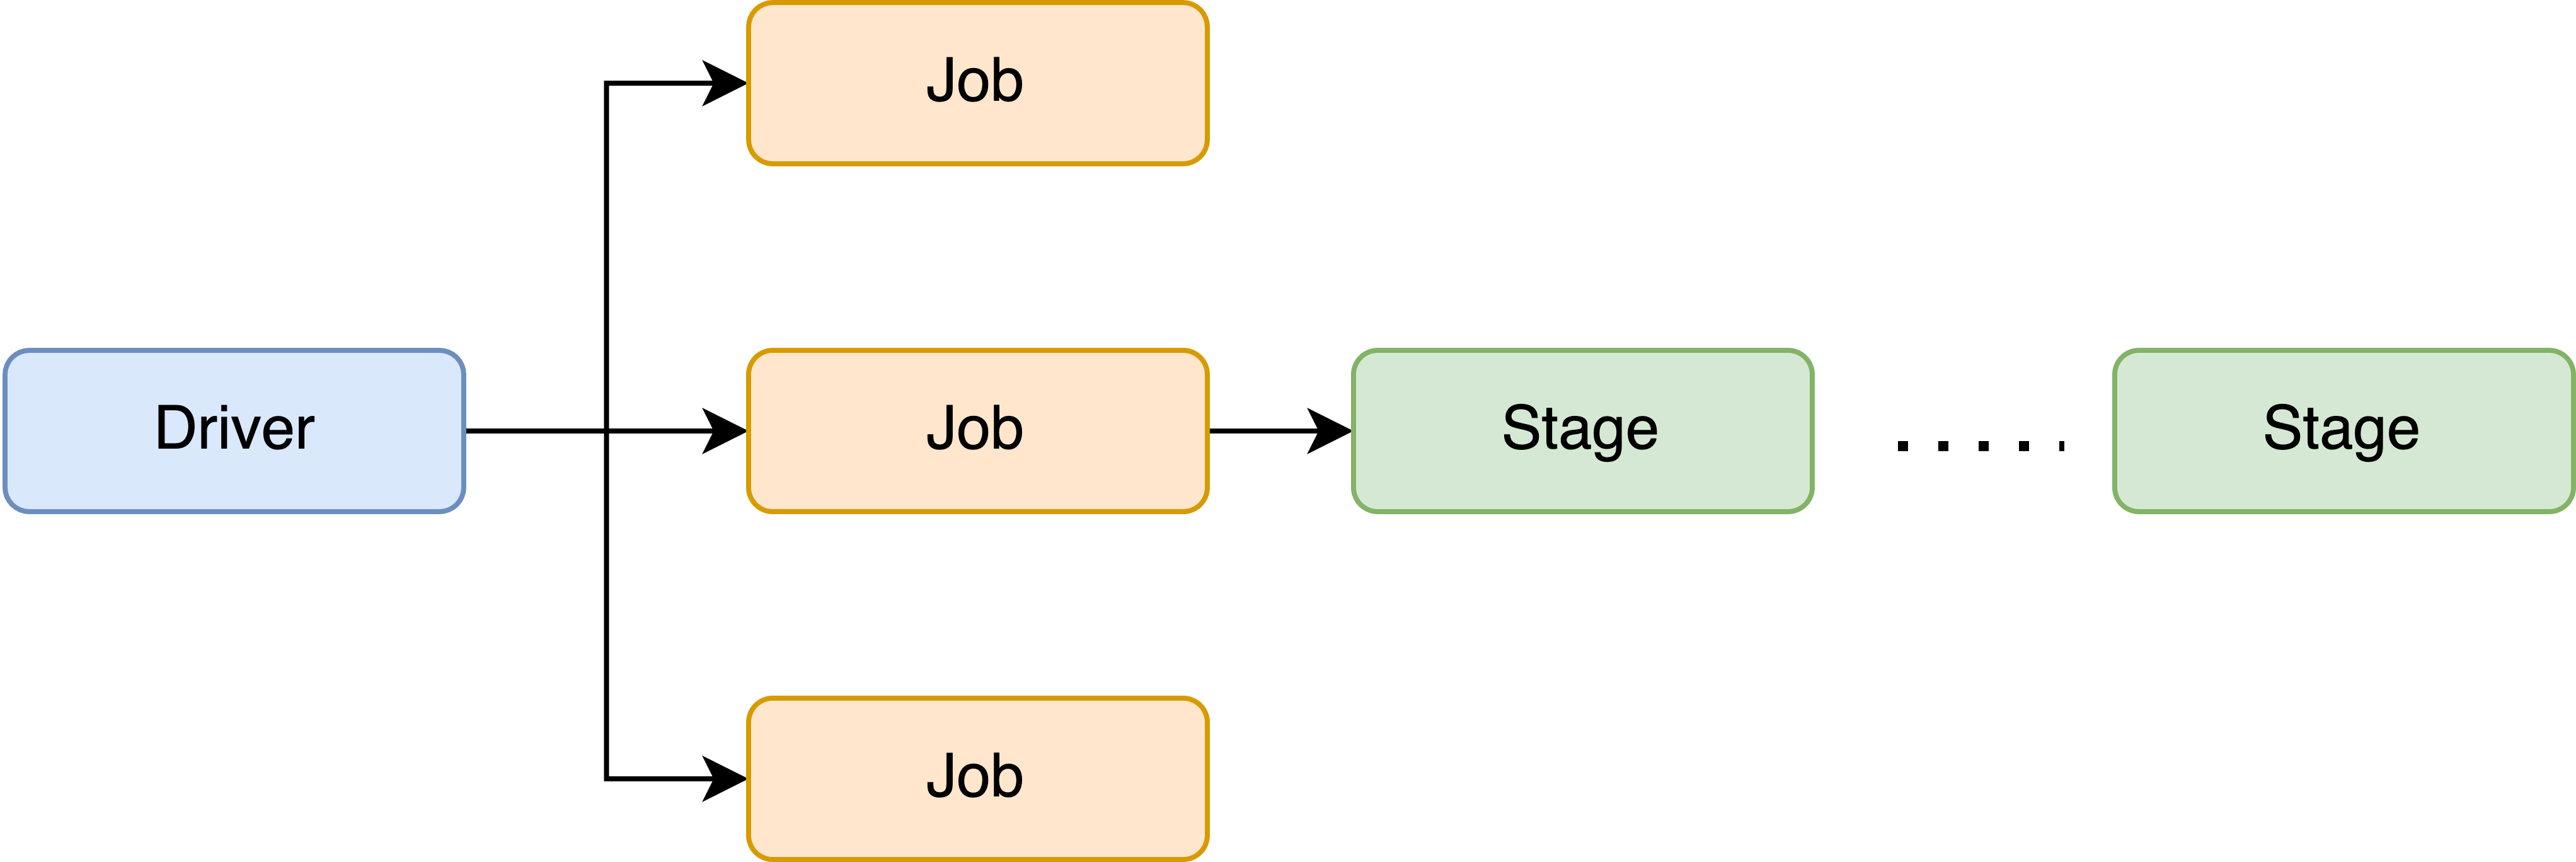
\includegraphics[width=\textwidth,height=.65\textheight,keepaspectratio]{./Figures/chapter-04/Spark_Stages}
        \caption{Spark job creating one or more stages}\label{fig:spark_stages}
    \end{figure}
\end{frame}
\begin{frame}
    \frametitle{Spark Stages}
    \begin{figure}
        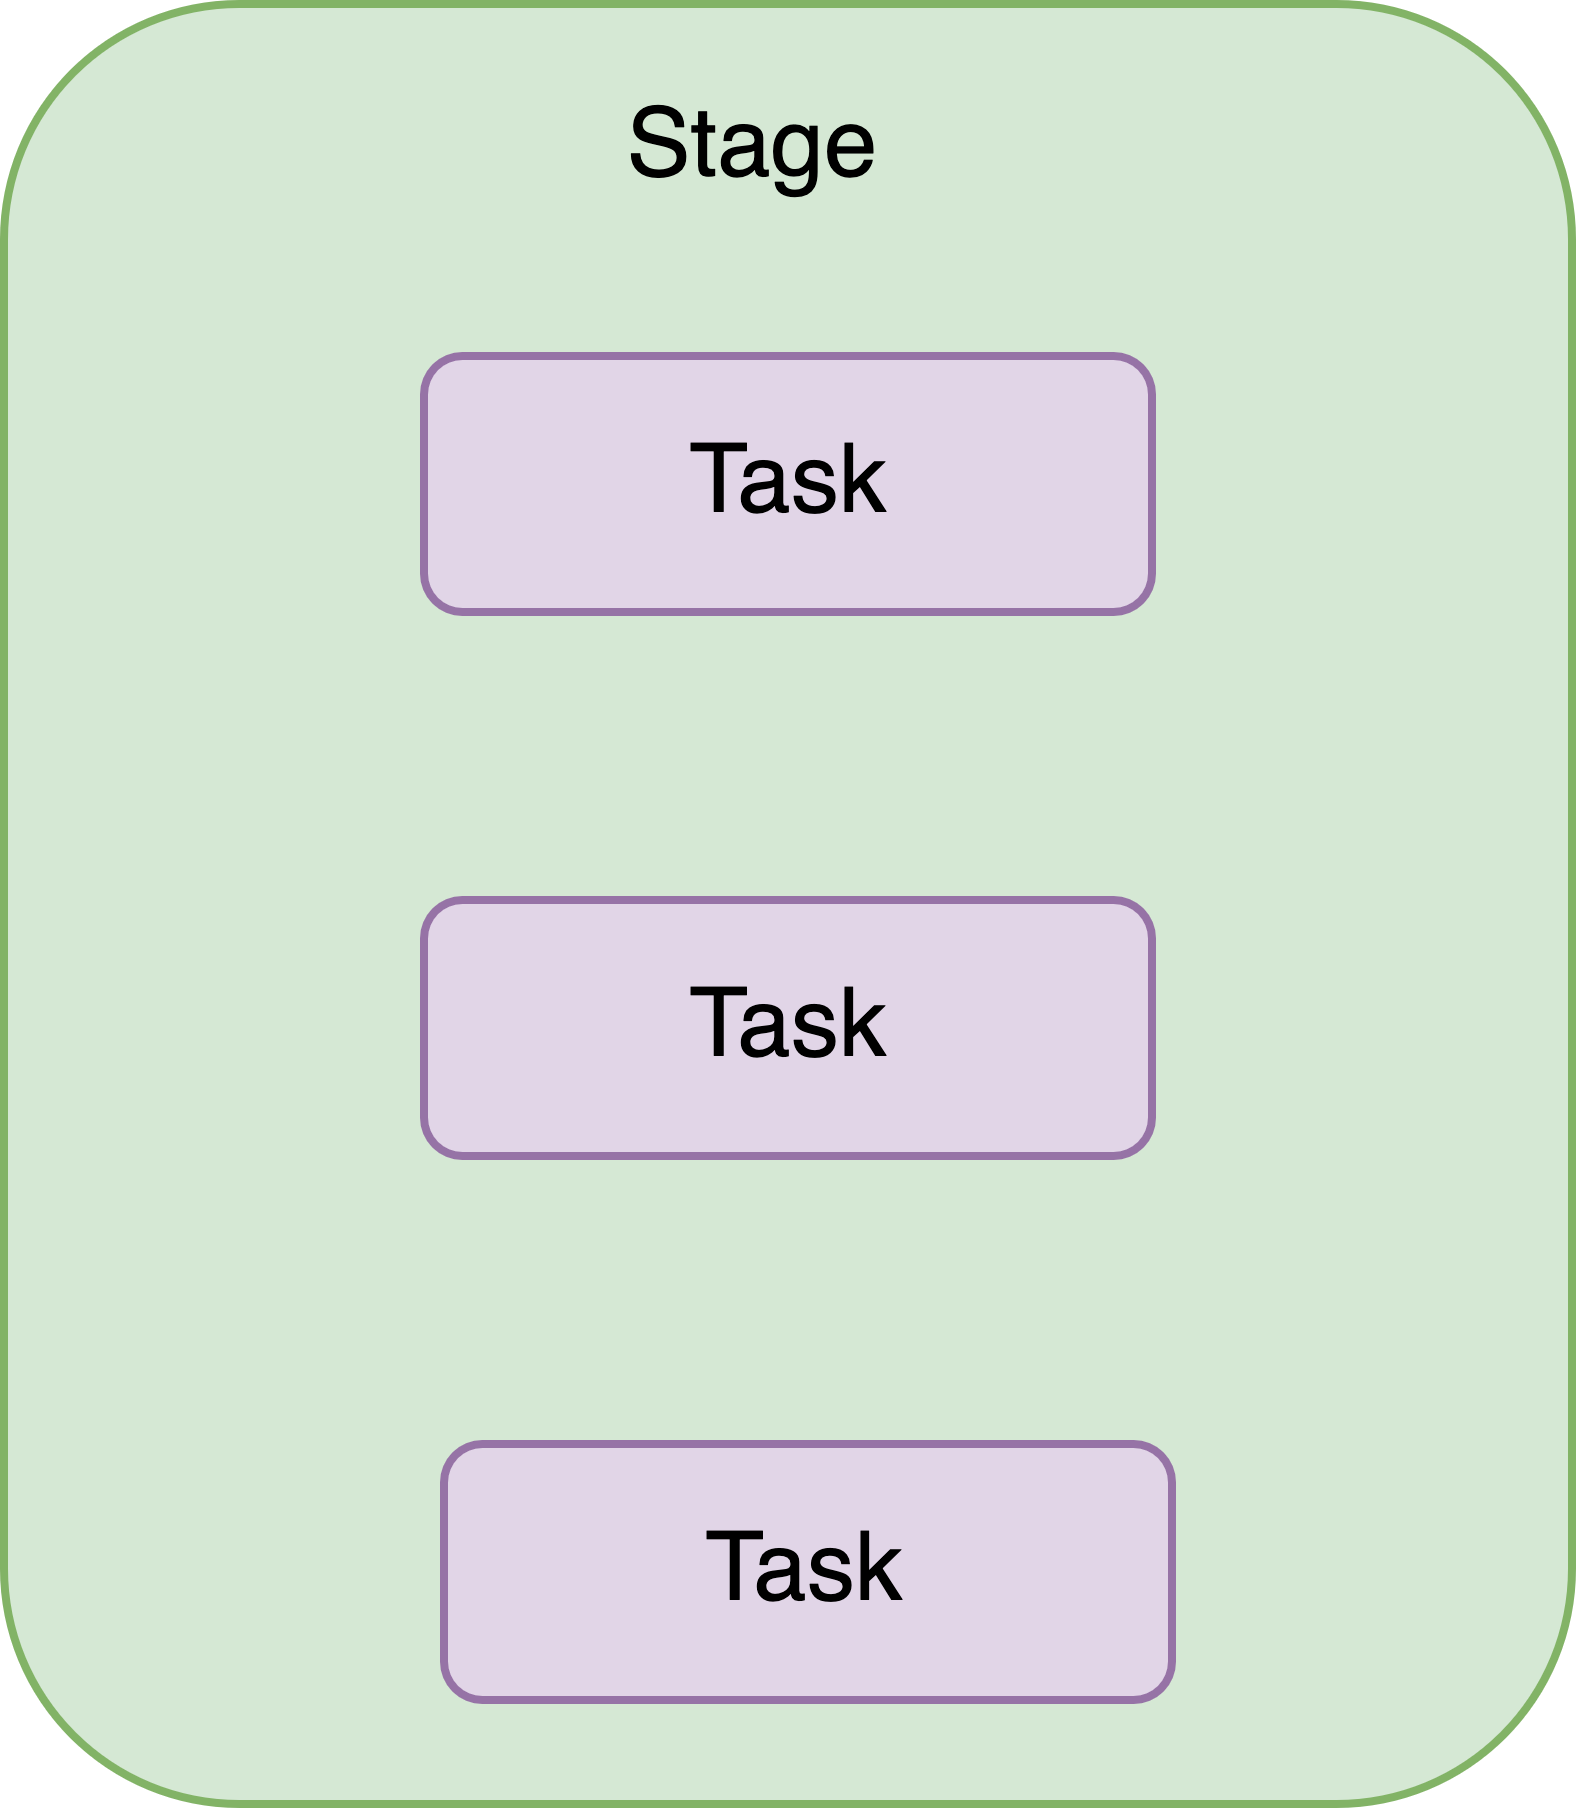
\includegraphics[width=\textwidth,height=.7\textheight,keepaspectratio]{./Figures/chapter-04/Spark_Stage}
        \caption{Spark stage creating one or more tasks to be distributed to executors}\label{fig:spark_stage}
    \end{figure}
\end{frame}
\begin{frame}
    \frametitle{Spark Tasks}
    \begin{figure}
        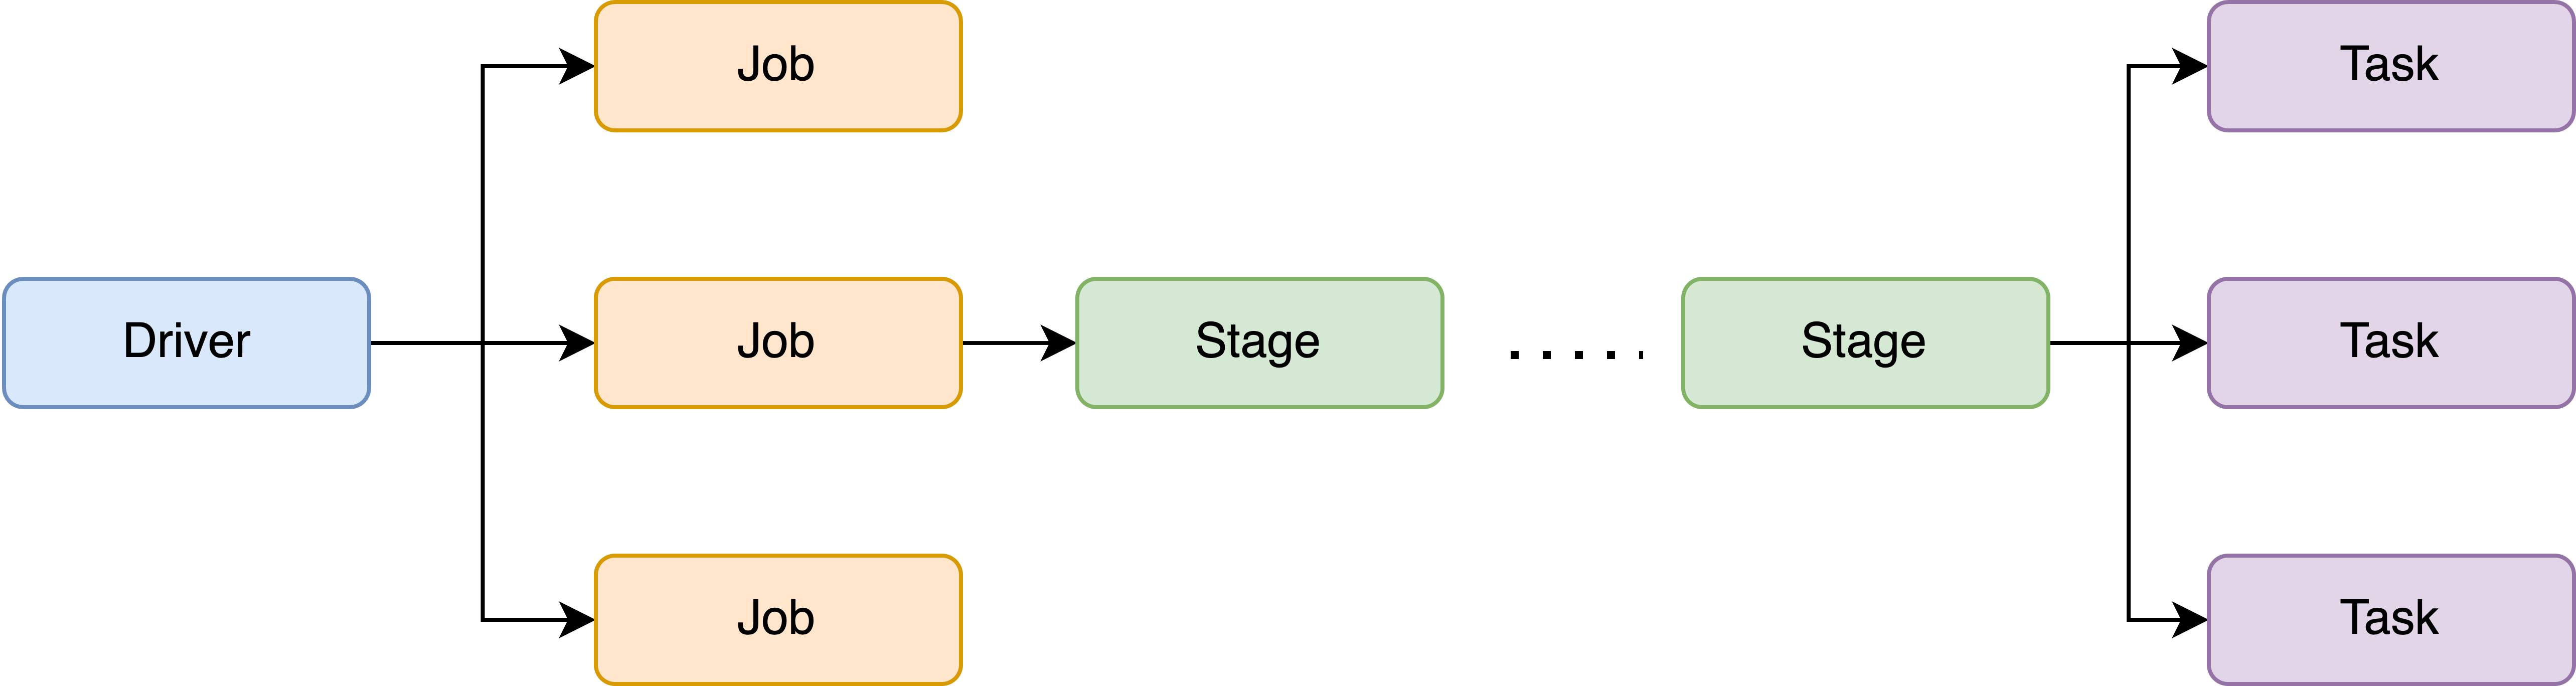
\includegraphics[width=\textwidth,height=.7\textheight,keepaspectratio]{./Figures/chapter-04/Spark_tasks}
        \caption{Spark stage creating one or more tasks to be distributed to executors}\label{fig:Spark_tasks}
    \end{figure}
\end{frame}

\subsection{Running Word Count \& Aggregation using Spark}\label{subsec:running-word-count-&-aggregation-using-spark}

\subsection{Spark Application Life Cycle}\label{subsec:spark-application-life-cycle}
%%%% Later
\begin{frame}
    \frametitle{The Life Cycle of a Spark Application (Inside Spark)}
    \begin{itemize}
        \item The Life Cycle of a Spark Application (Inside Spark)
    \end{itemize}
\end{frame}
\begin{frame}
    \frametitle{The Life Cycle of a Spark Application (Outside Spark)}
    \begin{itemize}
        \item The Life Cycle of a Spark Application (Outside Spark)
    \end{itemize}
\end{frame}
\begin{frame}
    \frametitle{The Life Cycle of a Spark Application (Inside Spark)}
    \begin{itemize}
        \item The Life Cycle of a Spark Application (Inside Spark)
    \end{itemize}
\end{frame}

\begin{frame}
    \frametitle{ADVANCED: SPARK DRIVER INTERNAL SCHEDULER}
    \begin{itemize}
        \item GOING DEEPER INTO SPARK DRIVER.
        \item CAN WE OPTIMIZE SPARK DRIVER WORKLOAD?
    \end{itemize}
\end{frame}
%%%%%%%%%%%%%%%%%%%%%%%%%%%%%%%%%%%%%%%%%%%%%%%%%%%%%%

\subsection{Further Readings and Assignment}


%%% Local Variables:
%%% mode: latex
%%% TeX-master: "../main"
% !TeX root = ../main.tex
%%% TeX-engine: xetex
%%% End:
%    \include{Ch04-Spark/FN-Scala}
%    \include{Ch04-Spark/Spark}
%    \include{Ch05-BigData-Applications/Applications}
%    \include{Ch06-Massaging-Systems/Massaging-Systems}
%    \include{Ch07-DataOrchestration/Orchestration}
%    \include{Ch08-NoSqlDB/NoSql}
%    \include{Ch09-Elastic/Elastic}
%    \include{Ch10-Architecture/Architecture}
%    \include{Appendix/Appendix}
%%%%%%%%%%%%%%%%%%%%%%%%%%%%%%%%%%%%%%%%%%%%%%%%%%%%%%

\begin{frame}[c]{ }
    \centering     
   
    \textcolor{offgreen}{ \large Thank you for watching!}
\end{frame}


\begin{frame}[c]{ }
    \centering 
    \textcolor{offyellow}{\large See you in the next video \Smiley{}}
\end{frame}
    %%%%%%%%%%%%%%%%%%%%%%%%%%%%%%%%%%%%%%%%%%%%%%%%%%%%%%%%%%%%%%%%%%%%%%%%%%%%%%%%%%%%%%%
\end{document}

%%% Local Variables:
%%% mode: latex
%%% TeX-master: t
%%% TeX-engine: xetex
%%% End:
